\appendix
\renewcommand{\thechapter}{B}
\renewcommand{\chaptername}{Appendix}

\chapter{Experimental and FDS Data Plots}
\label{chap:exp_FDS_plots}

\section{Temperature}
\subsection*{\textit{Hot Gas Layer Temperatures}}
\begin{figure}[!h]
	\centering
	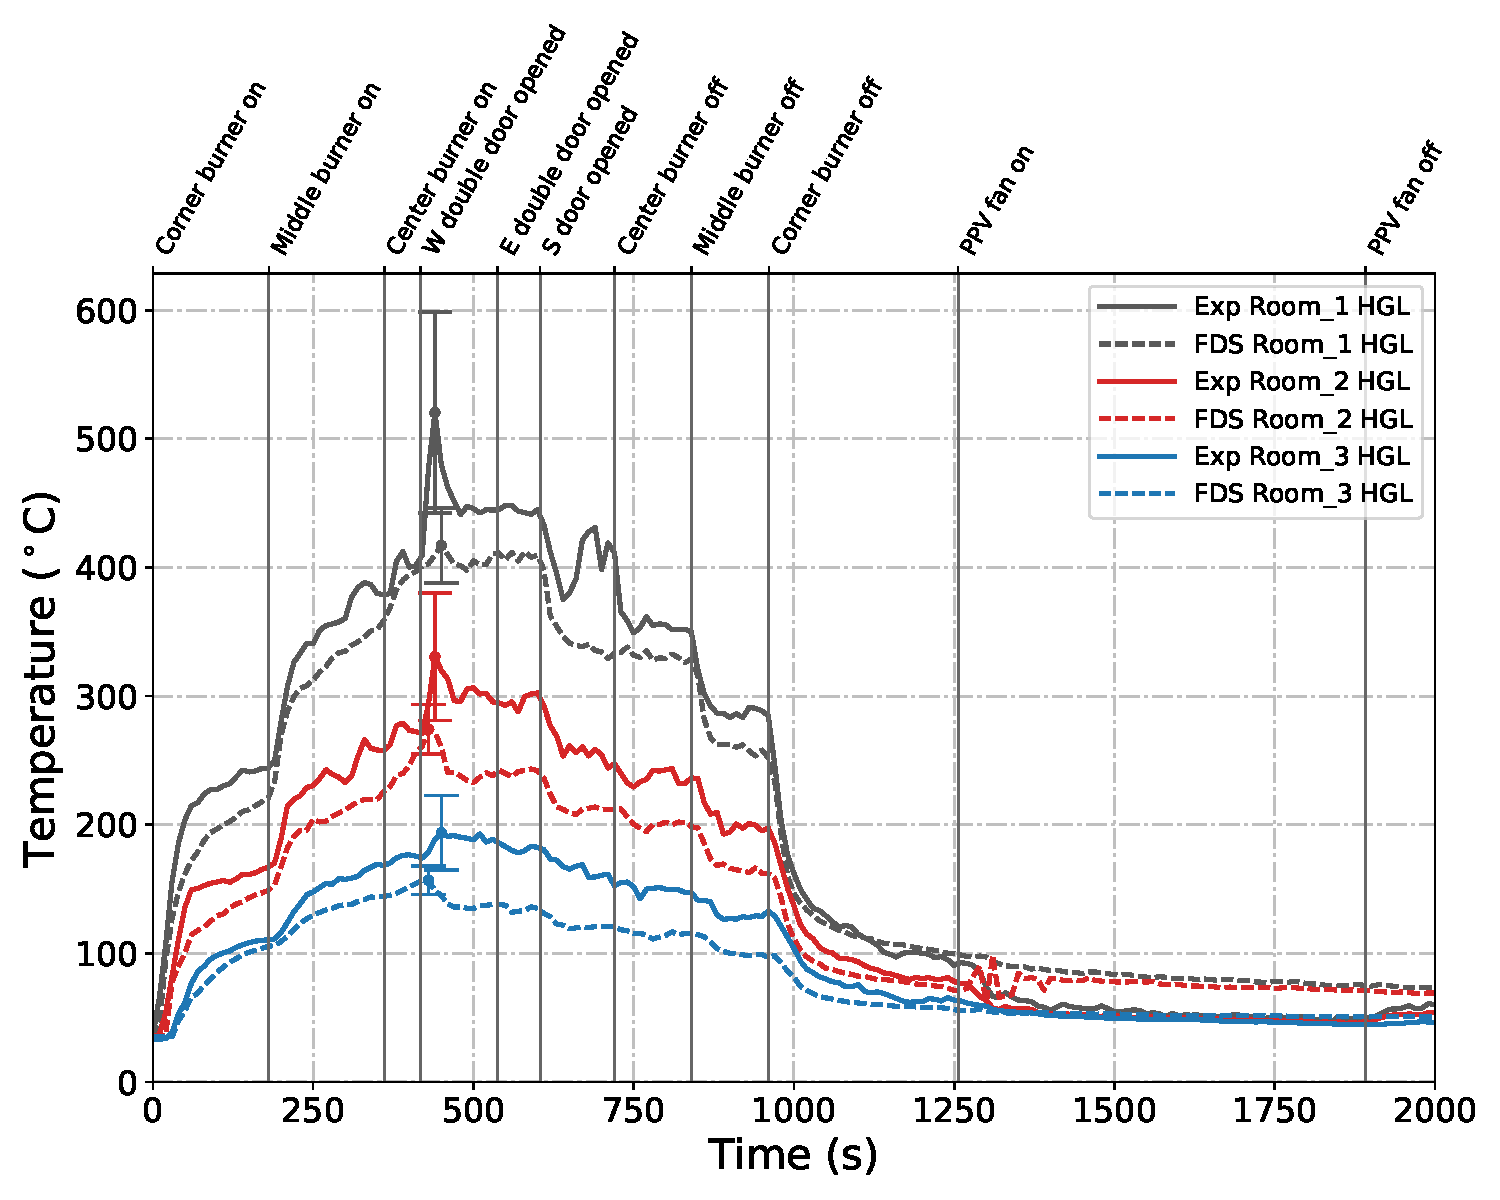
\includegraphics[width=\columnwidth]{../../Plots/Validation/Temperature/Test_2_HGL}
	\caption[Plots of measured and predicted hot gas layer temperatures during Test~2.]{Plots of measured and predicted hot gas layer temperatures in the three rooms of the East Structure during Test~2.}
	\label{fig:HGL_data_Test2}
\end{figure}

\begin{figure}[!h]
	\centering
	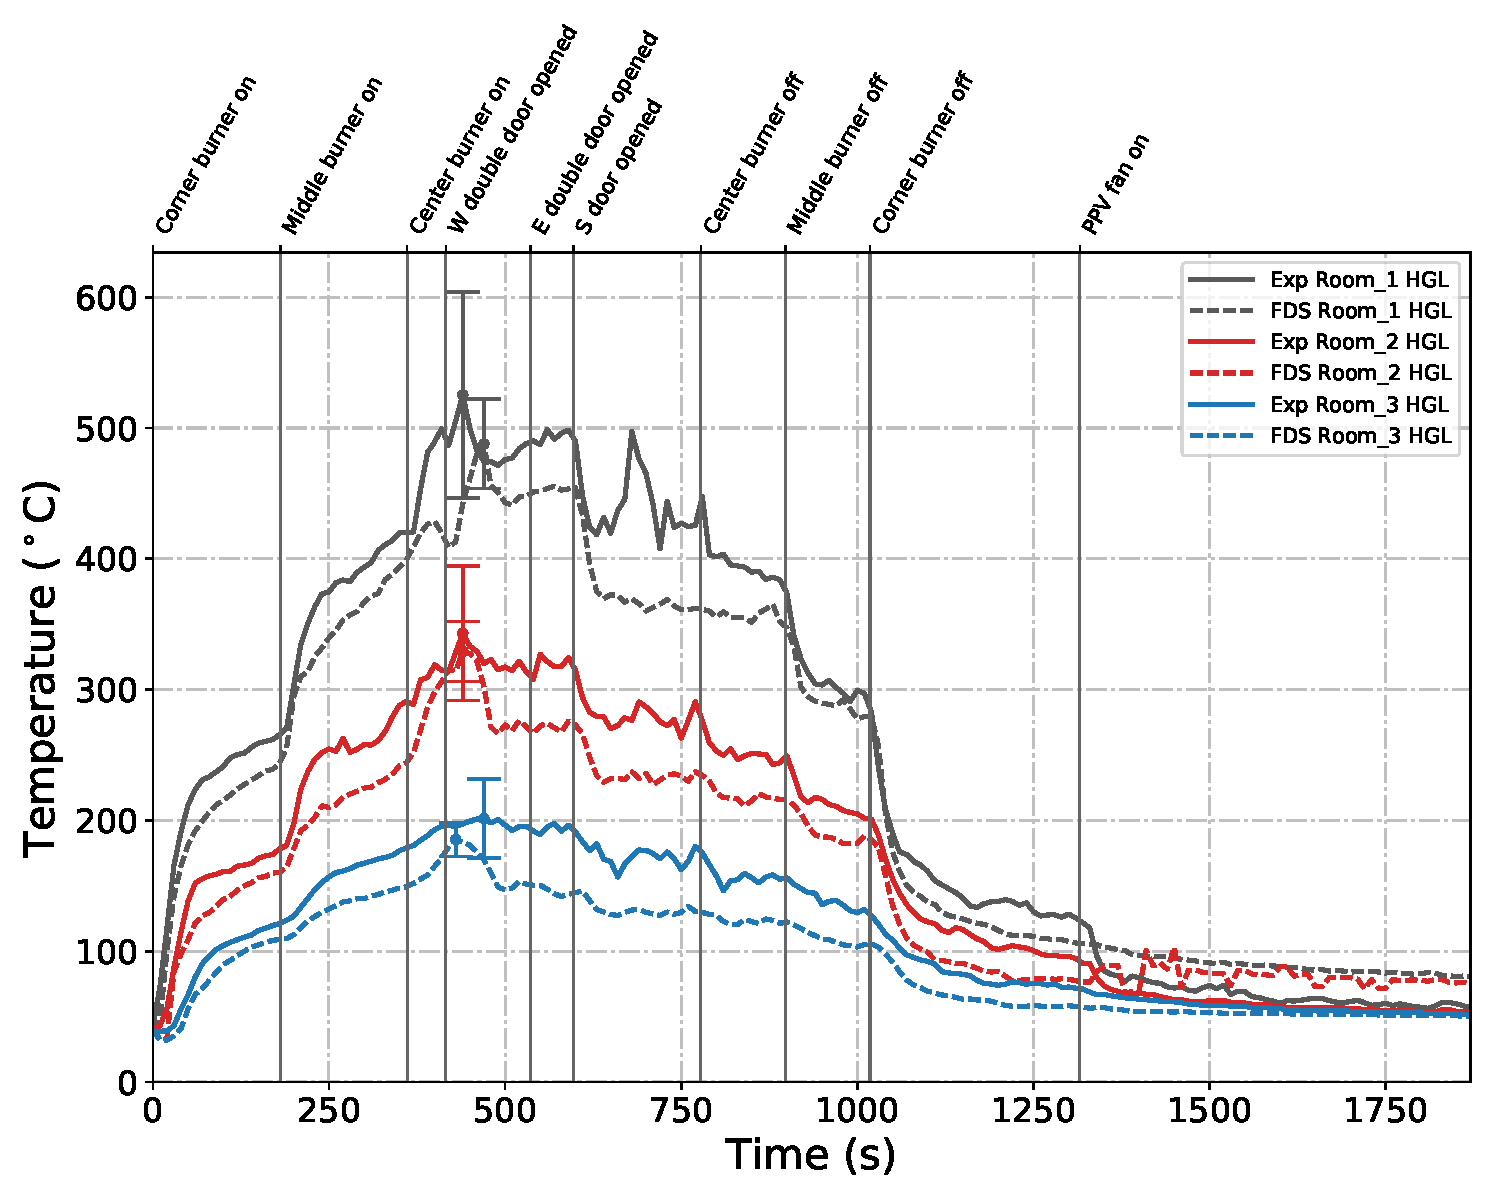
\includegraphics[width=\columnwidth]{../../Plots/Validation/Temperature/Test_3_HGL}
	\caption[Plots of measured and predicted hot gas layer temperatures during Test~3.]{Plots of measured and predicted hot gas layer temperatures in the three rooms of the East Structure during Test~3.}
	\label{fig:HGL_data_Test3}
\end{figure}

\begin{figure}[!h]
	\centering
	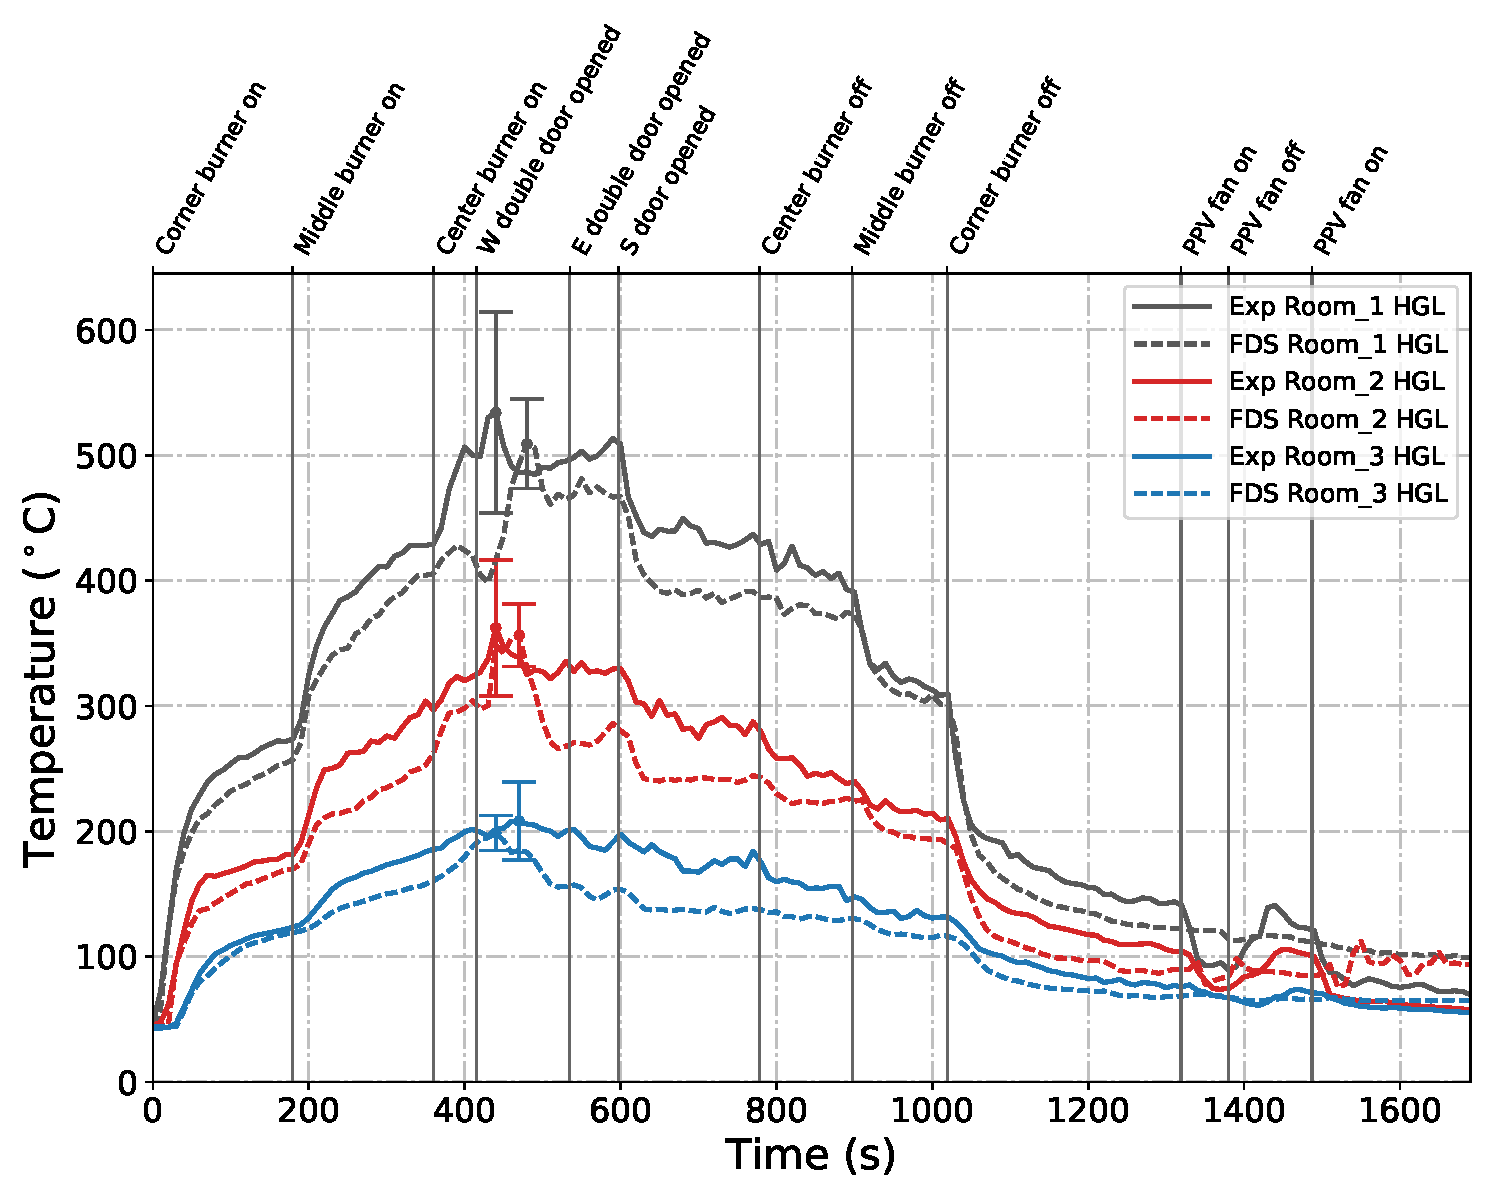
\includegraphics[width=\columnwidth]{../../Plots/Validation/Temperature/Test_4_HGL}
	\caption[Plots of measured and predicted hot gas layer temperatures during Test~4.]{Plots of measured and predicted hot gas layer temperatures in the three rooms of the East Structure during Test~4.}
	\label{fig:HGL_data_Test4}
\end{figure}

\begin{figure}[!h]
	\centering
	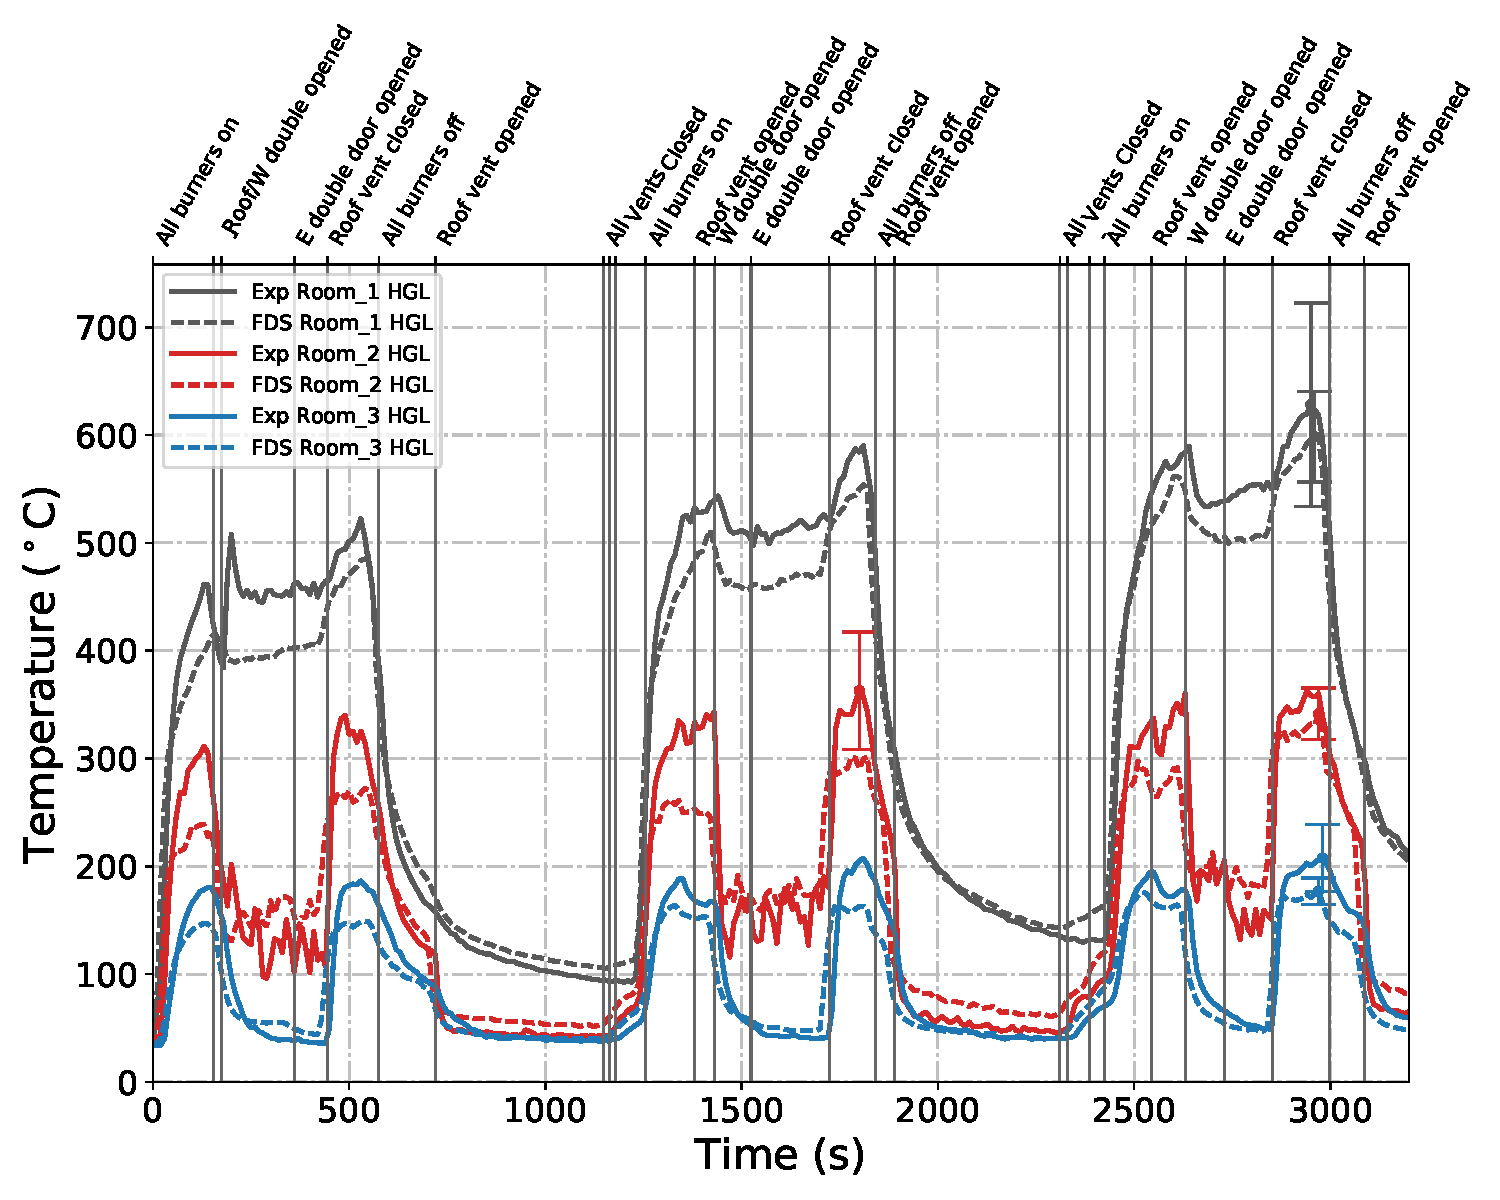
\includegraphics[width=\columnwidth]{../../Plots/Validation/Temperature/Test_5_HGL}
	\caption[Plots of measured and predicted hot gas layer temperatures during Test~5.]{Plots of measured and predicted hot gas layer temperatures in the three rooms of the East Structure during Test~5.}
	\label{fig:HGL_data_Test5}
\end{figure}

\begin{figure}[!h]
	\centering
	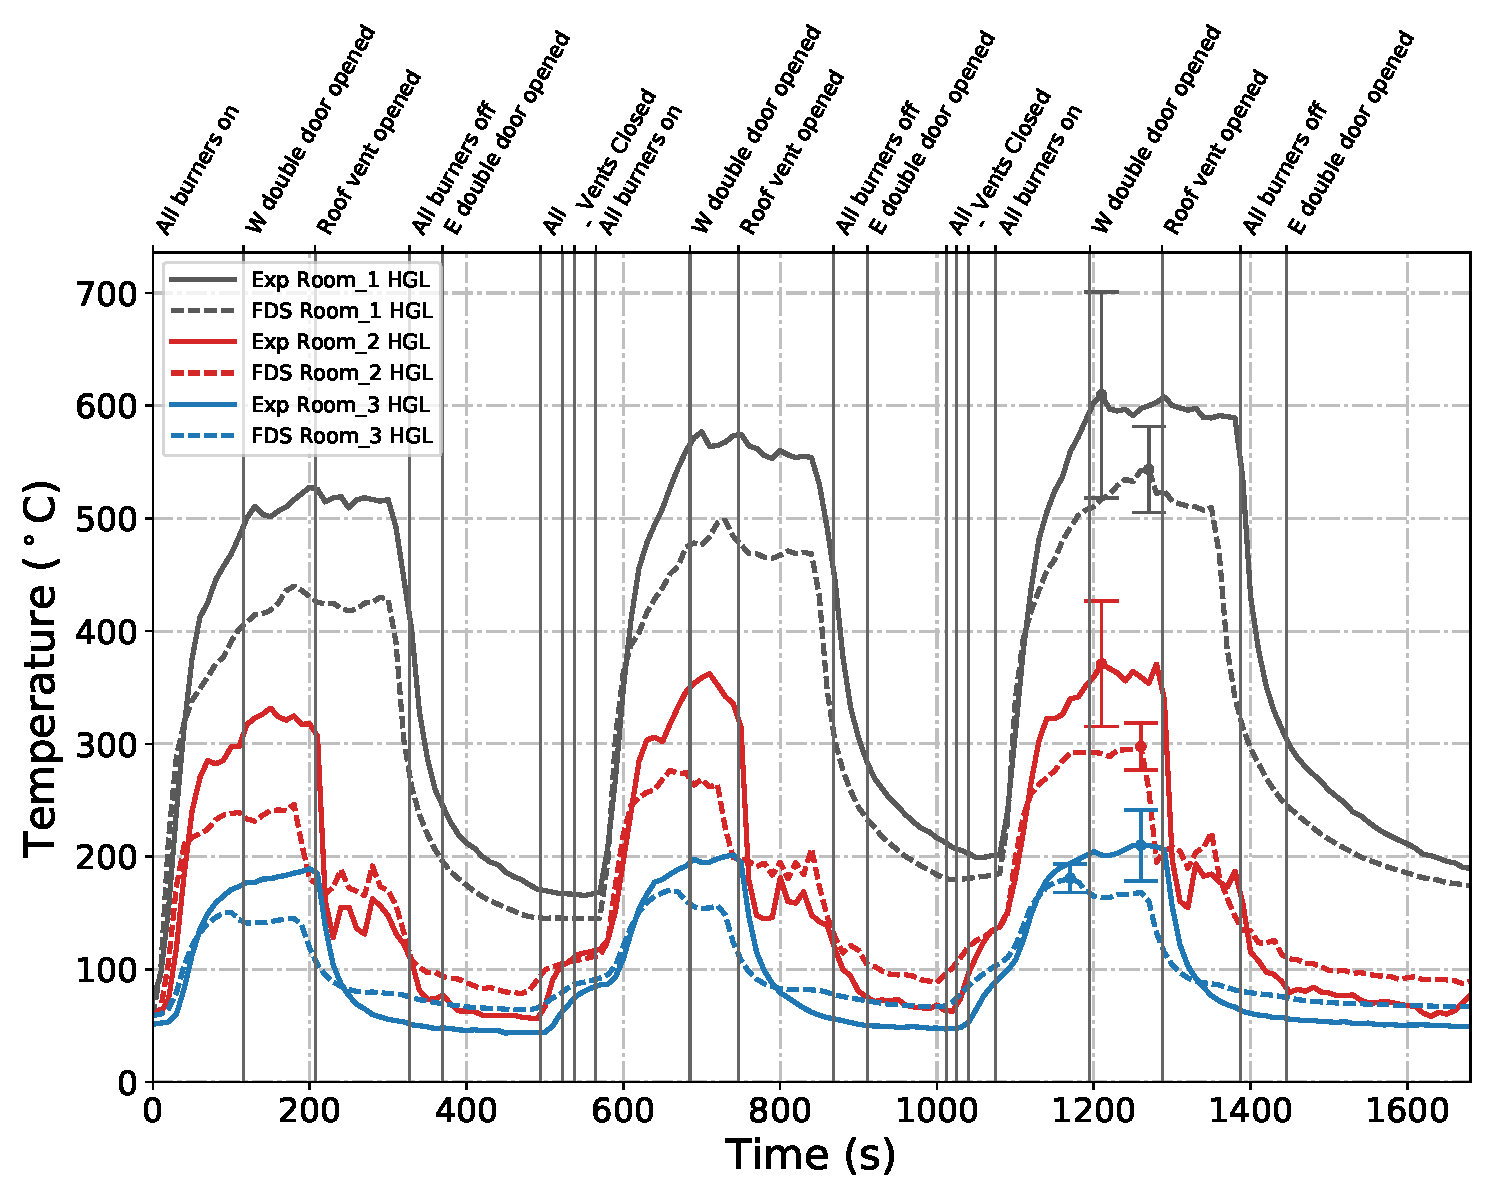
\includegraphics[width=\columnwidth]{../../Plots/Validation/Temperature/Test_6_HGL}
	\caption[Plots of measured and predicted hot gas layer temperatures during Test~6.]{Plots of measured and predicted hot gas layer temperatures in the three rooms of the East Structure during Test~6.}
	\label{fig:HGL_data_Test6}
\end{figure}

\begin{figure}[!h]
	\centering
	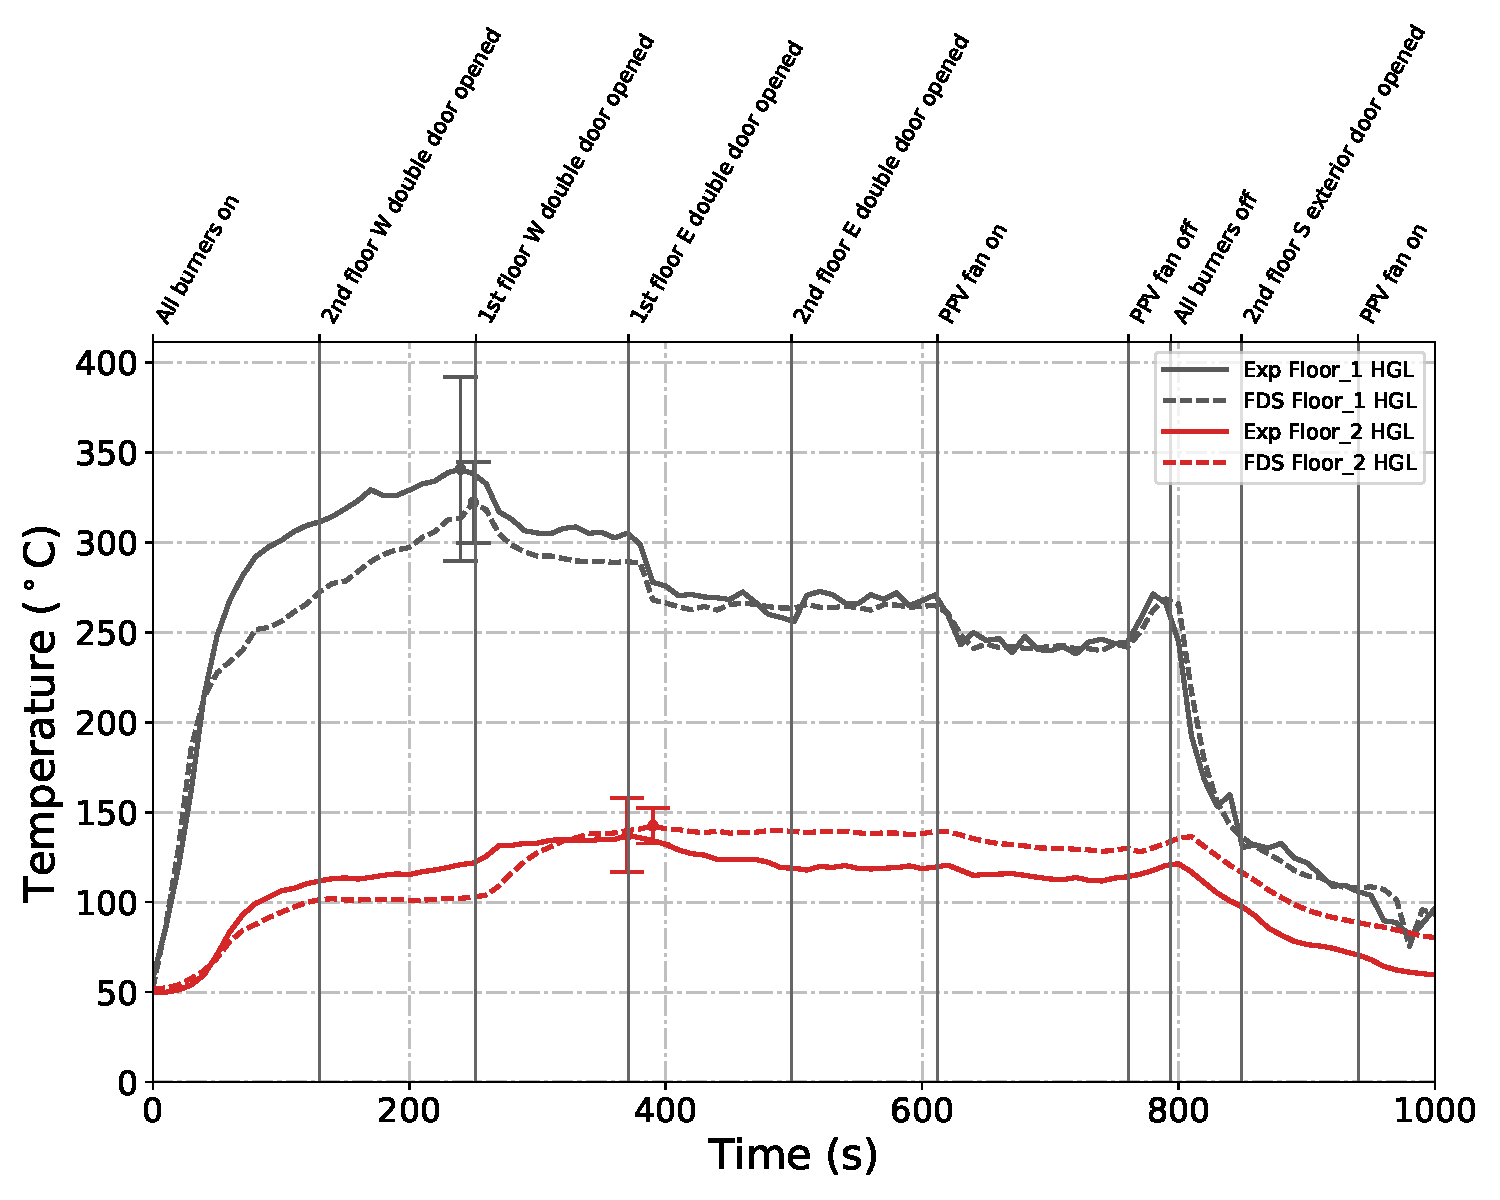
\includegraphics[width=\columnwidth]{../../Plots/Validation/Temperature/Test_23_HGL}
	\caption[Plots of measured and predicted hot gas layer temperatures during Test~23.]{Plots of measured and predicted hot gas layer temperatures on the first and second floors of the West Structure during Test~23.}
	\label{fig:HGL_data_Test23}
\end{figure}

\begin{figure}[!h]
	\centering
	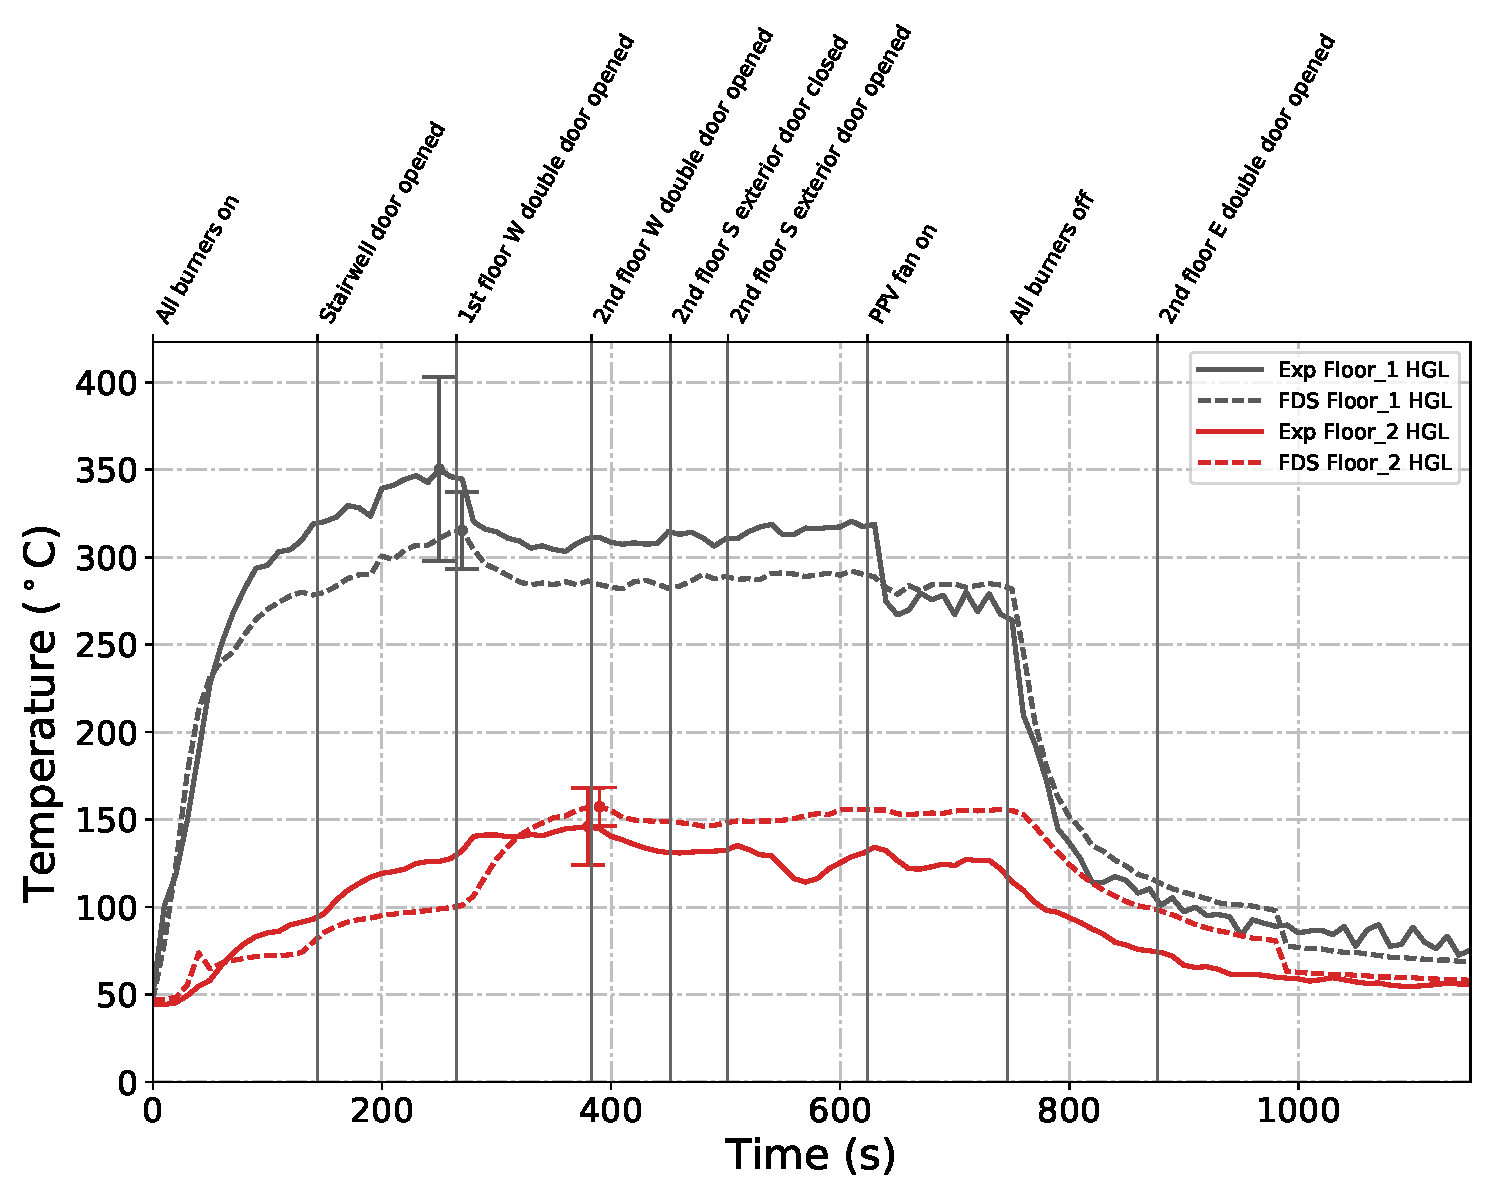
\includegraphics[width=\columnwidth]{../../Plots/Validation/Temperature/Test_24_HGL}
	\caption[Plots of measured and predicted hot gas layer temperatures during Test~24.]{Plots of measured and predicted hot gas layer temperatures on the first and second floors of the West Structure during Test~24.}
	\label{fig:HGL_data_Test24}
\end{figure}

\begin{figure}[!h]
	\centering
	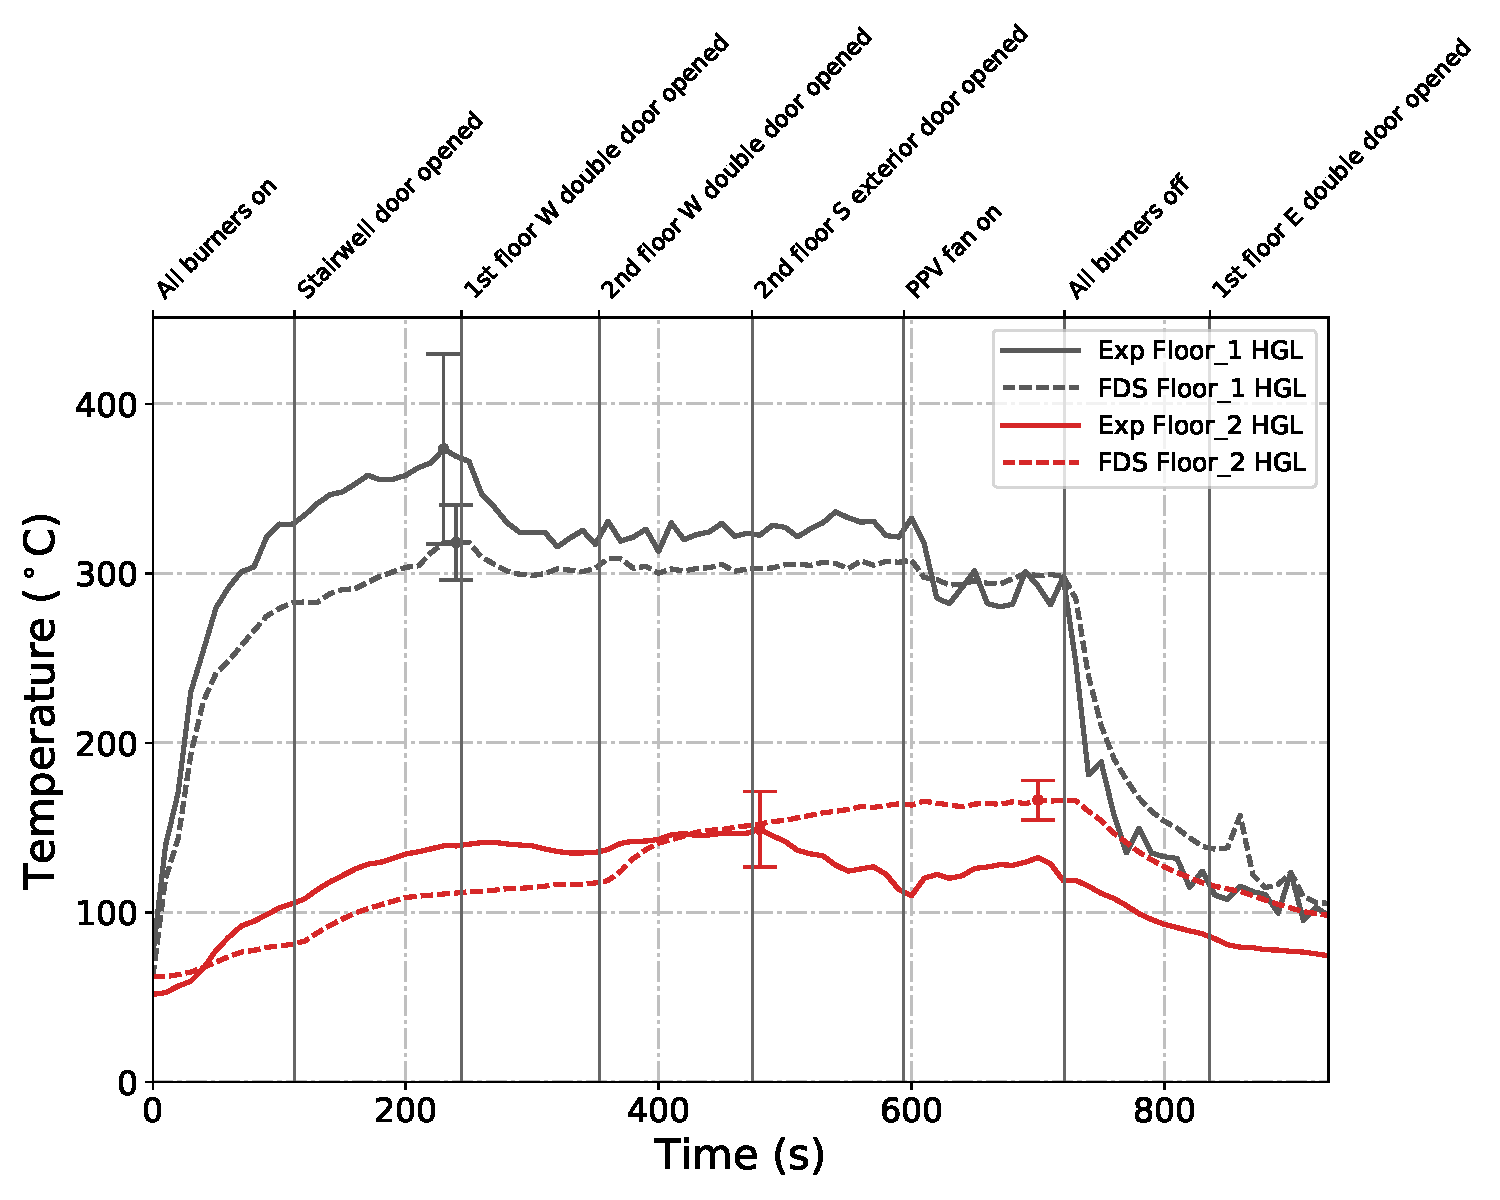
\includegraphics[width=\columnwidth]{../../Plots/Validation/Temperature/Test_25_HGL}
	\caption[Plots of measured and predicted hot gas layer temperatures during Test~25.]{Plots of measured and predicted hot gas layer temperatures on the first and second floors of the West Structure during Test~25.}
	\label{fig:HGL_data_Test25}
\end{figure}

\clearpage
\subsection*{\textit{Ceiling Jet Temperatures}}
\begin{figure}[!h]
	\centering
	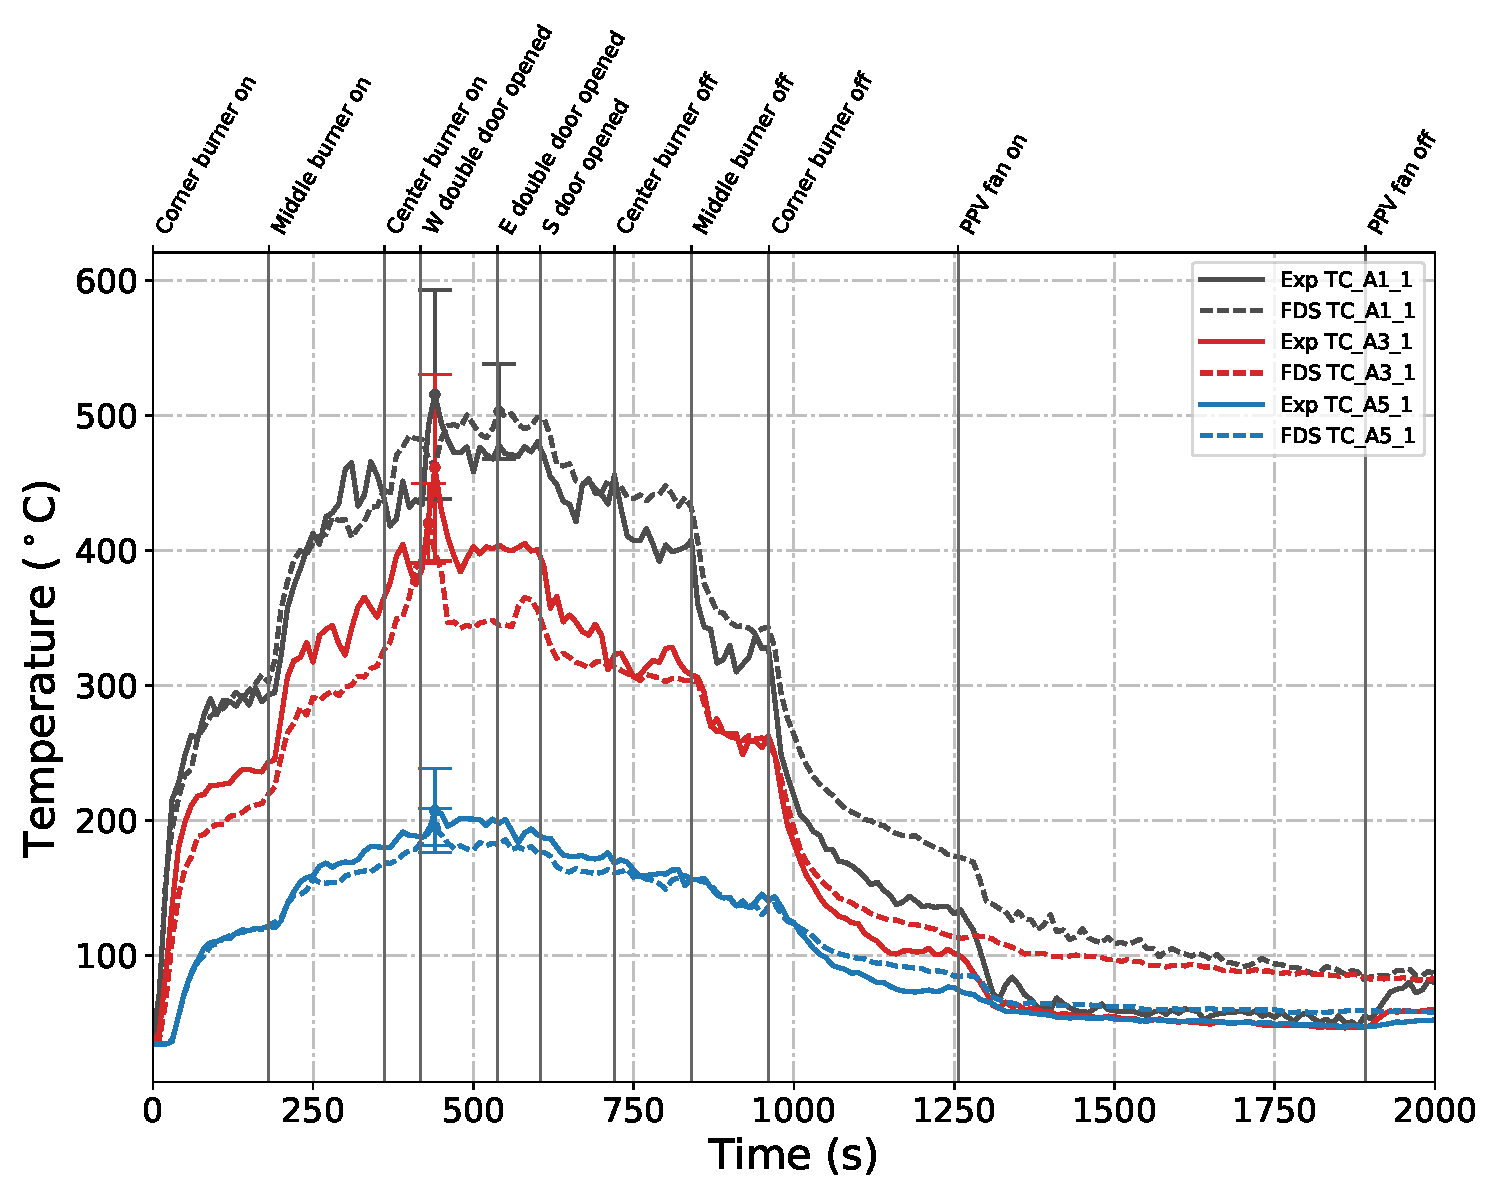
\includegraphics[width=\columnwidth]{../../Plots/Validation/Temperature/Test_2_cjet_1}
	\caption[Plots of measured and predicted ceiling jet temperatures during Test~2.]{Plots of measured and predicted ceiling jet temperatures during Test~2 obtained from thermocouple arrays A1, A3, and A5 located in the fire room, middle room, and north room of the East Structure, respectively.}
	\label{fig:cjet1_data_Test2}
\end{figure}

\begin{figure}[!h]
	\centering
	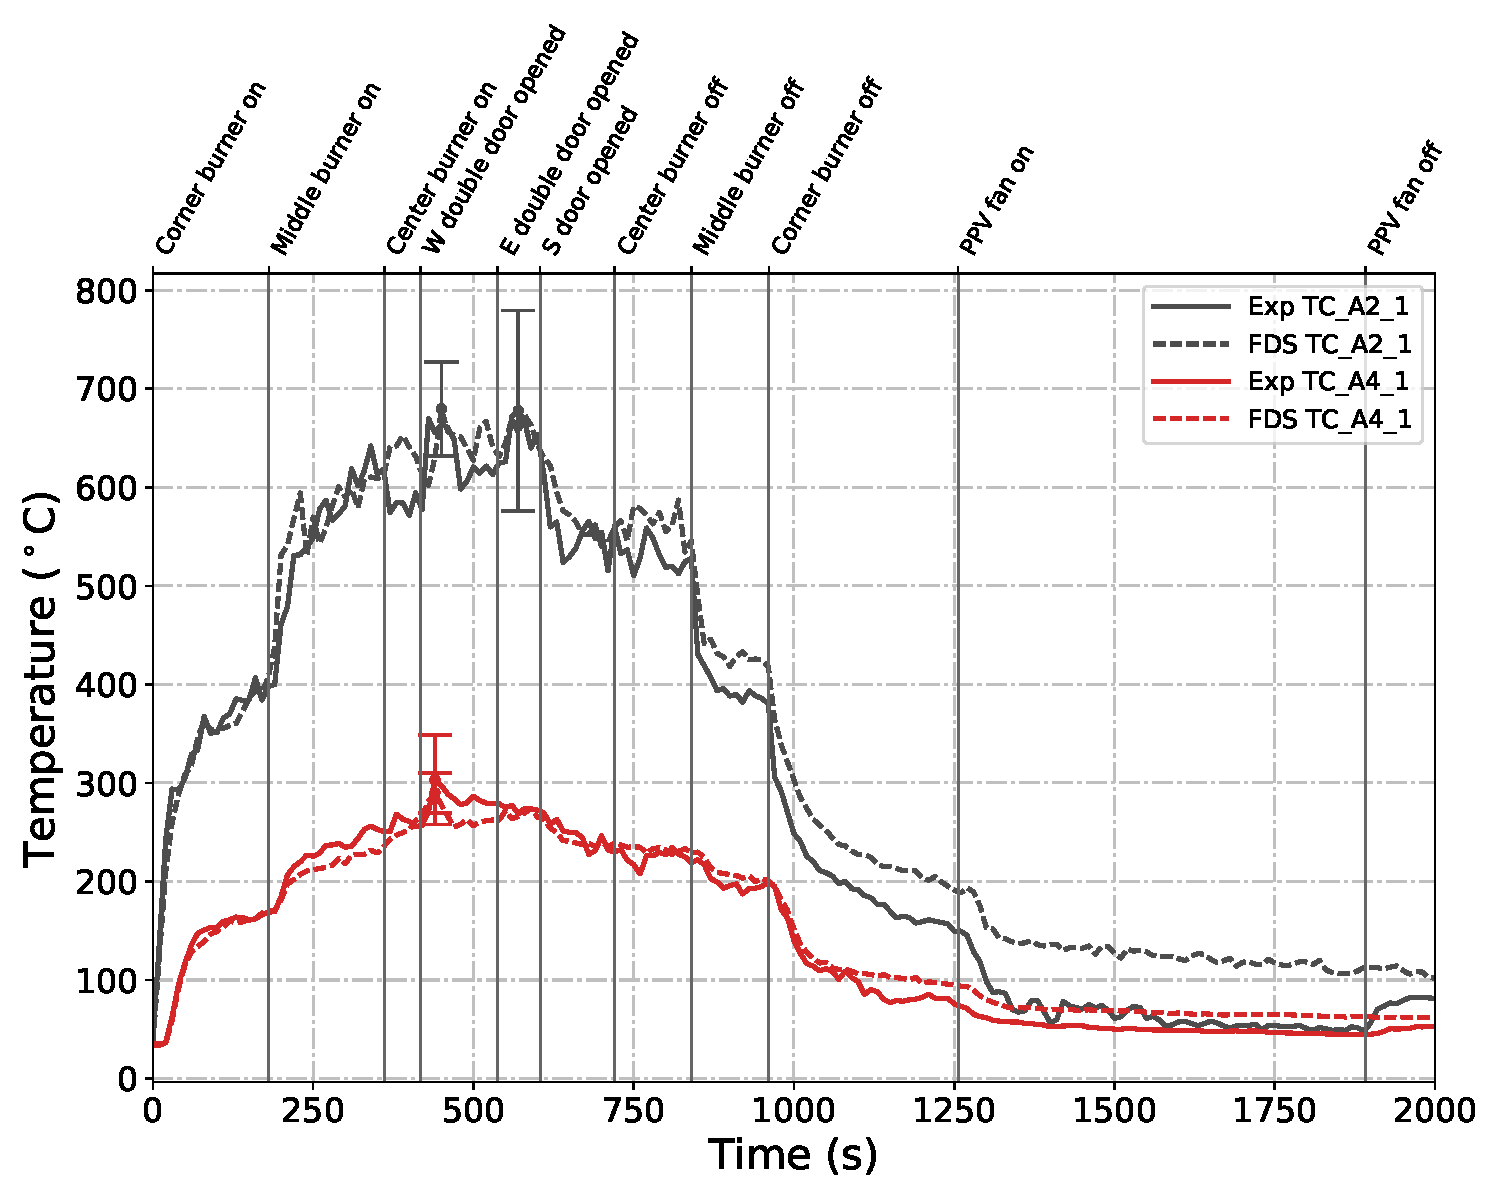
\includegraphics[width=\columnwidth]{../../Plots/Validation/Temperature/Test_2_cjet_2}
	\caption[Plots of measured and predicted ceiling jet temperatures during Test~2.]{Plots of measured and predicted ceiling jet temperatures during Test~2 obtained from thermocouple arrays A2 and A4 located in the fire room and north room of the East Structure, respectively.}
	\label{fig:cjet2_data_Test2}
\end{figure}

\begin{figure}[!h]
	\centering
	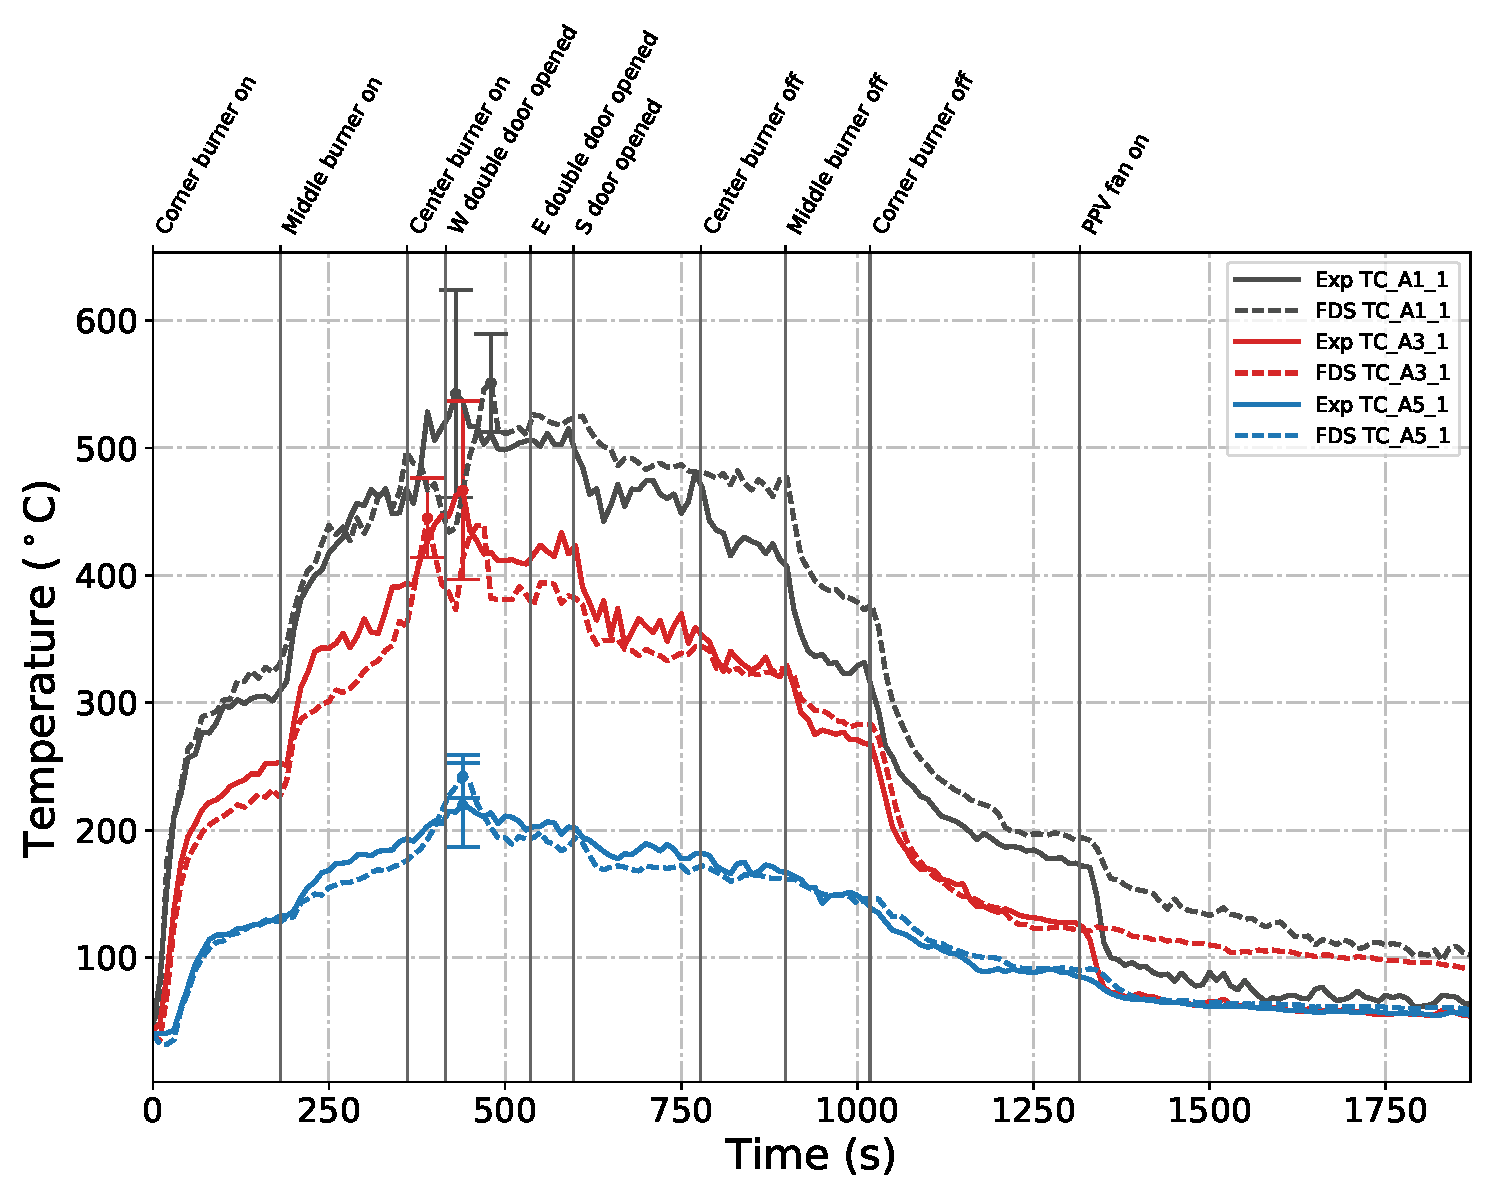
\includegraphics[width=\columnwidth]{../../Plots/Validation/Temperature/Test_3_cjet_1}
	\caption[Plots of measured and predicted ceiling jet temperatures during Test~3.]{Plots of measured and predicted ceiling jet temperatures during Test~3 obtained from thermocouple arrays A1, A3, and A5 located in the fire room, middle room, and north room of the East Structure, respectively.}
	\label{fig:cjet1_data_Test3}
\end{figure}

\begin{figure}[!h]
	\centering
	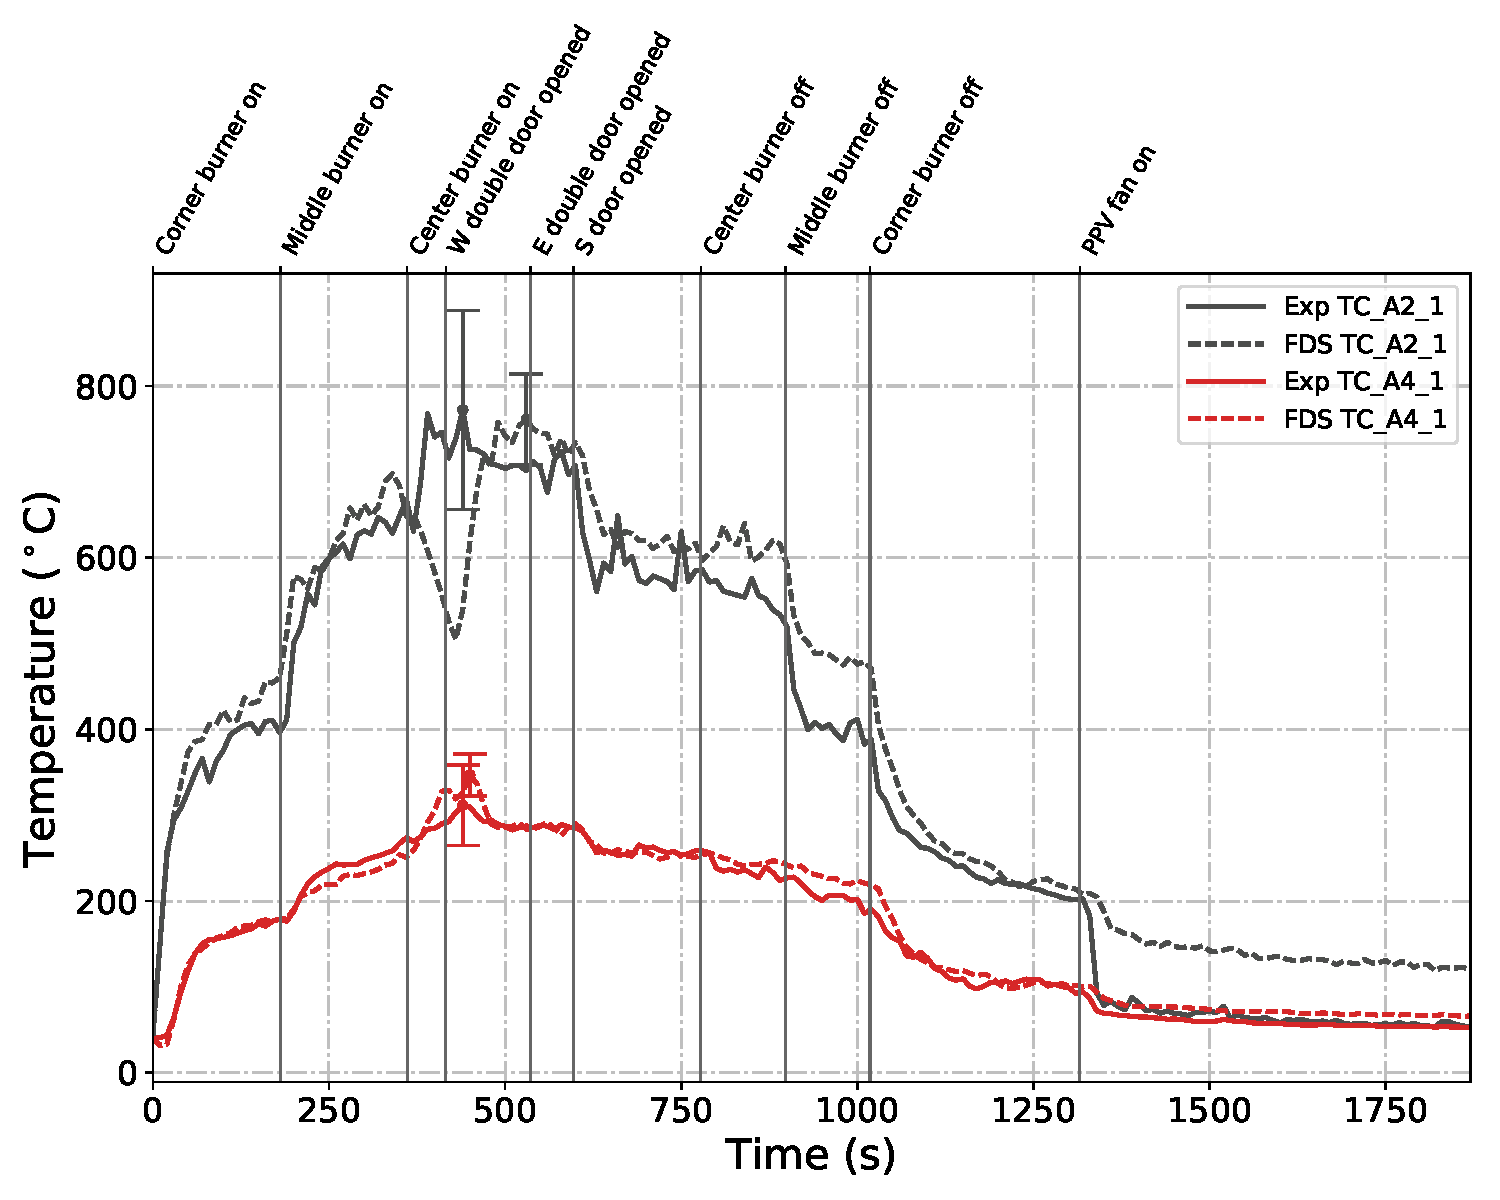
\includegraphics[width=\columnwidth]{../../Plots/Validation/Temperature/Test_3_cjet_2}
	\caption[Plots of measured and predicted ceiling jet temperatures during Test~3.]{Plots of measured and predicted ceiling jet temperatures during Test~3 obtained from thermocouple arrays A2 and A4 located in the fire room and north room of the East Structure, respectively.}
	\label{fig:cjet2_data_Test3}
\end{figure}

\begin{figure}[!h]
	\centering
	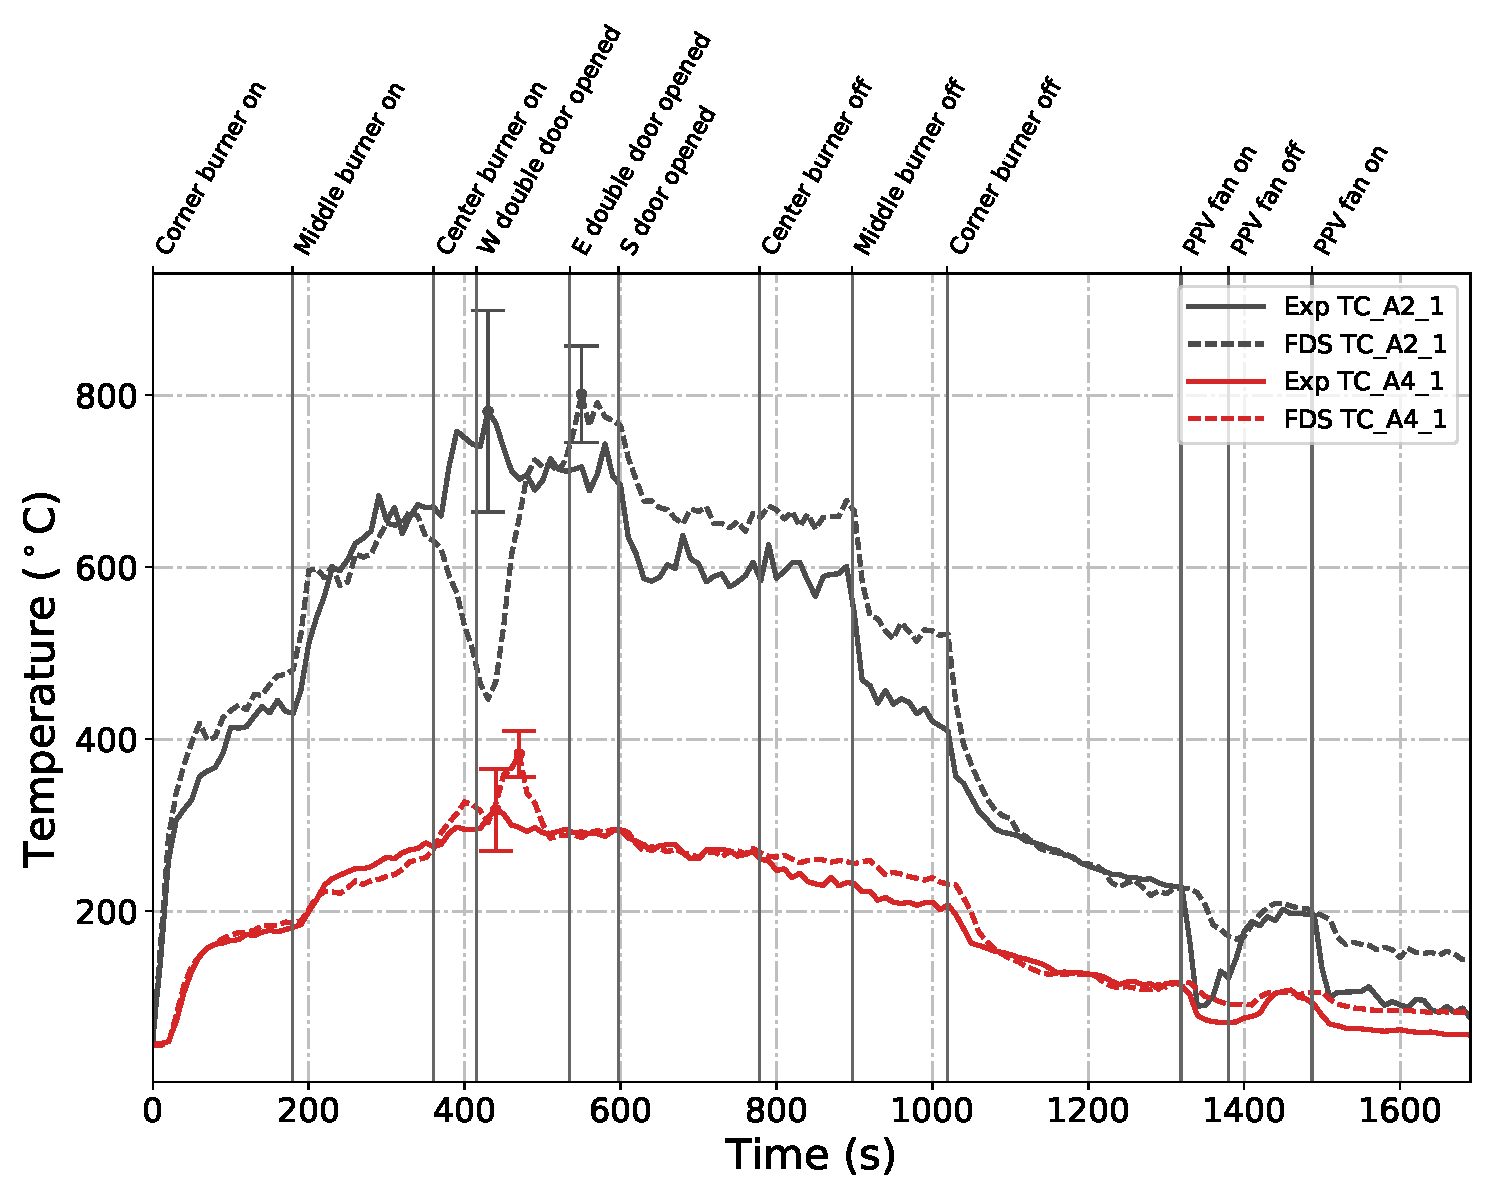
\includegraphics[width=\columnwidth]{../../Plots/Validation/Temperature/Test_4_cjet_2}
	\caption[Plots of measured and predicted ceiling jet temperatures during Test~4.]{Plots of measured and predicted ceiling jet temperatures during Test~4 obtained from thermocouple arrays A2 and A4 located in the fire room and north room of the East Structure, respectively.}
	\label{fig:cjet2_data_Test4}
\end{figure}

\begin{figure}[!h]
	\centering
	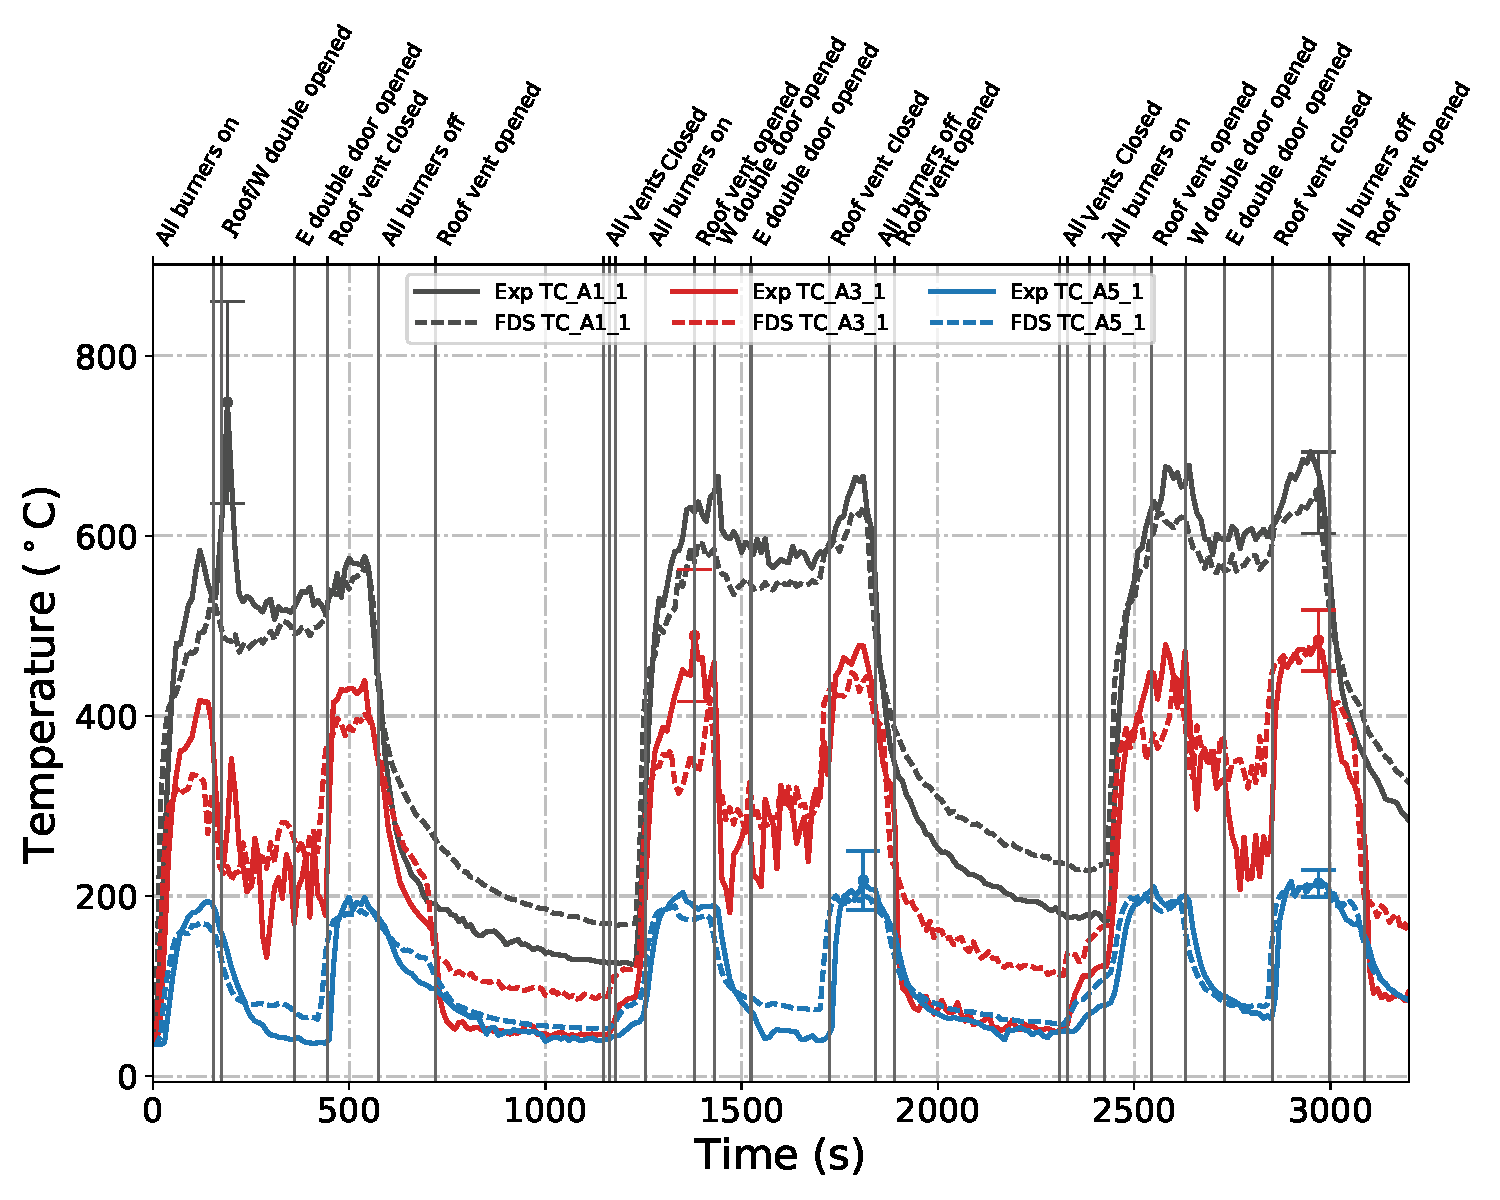
\includegraphics[width=\columnwidth]{../../Plots/Validation/Temperature/Test_5_cjet_1}
	\caption[Plots of measured and predicted ceiling jet temperatures during Test~5.]{Plots of measured and predicted ceiling jet temperatures during Test~5 obtained from thermocouple arrays A1, A3, and A5 located in the fire room, middle room, and north room of the East Structure, respectively.}
	\label{fig:cjet1_data_Test5}
\end{figure}

\begin{figure}[!h]
	\centering
	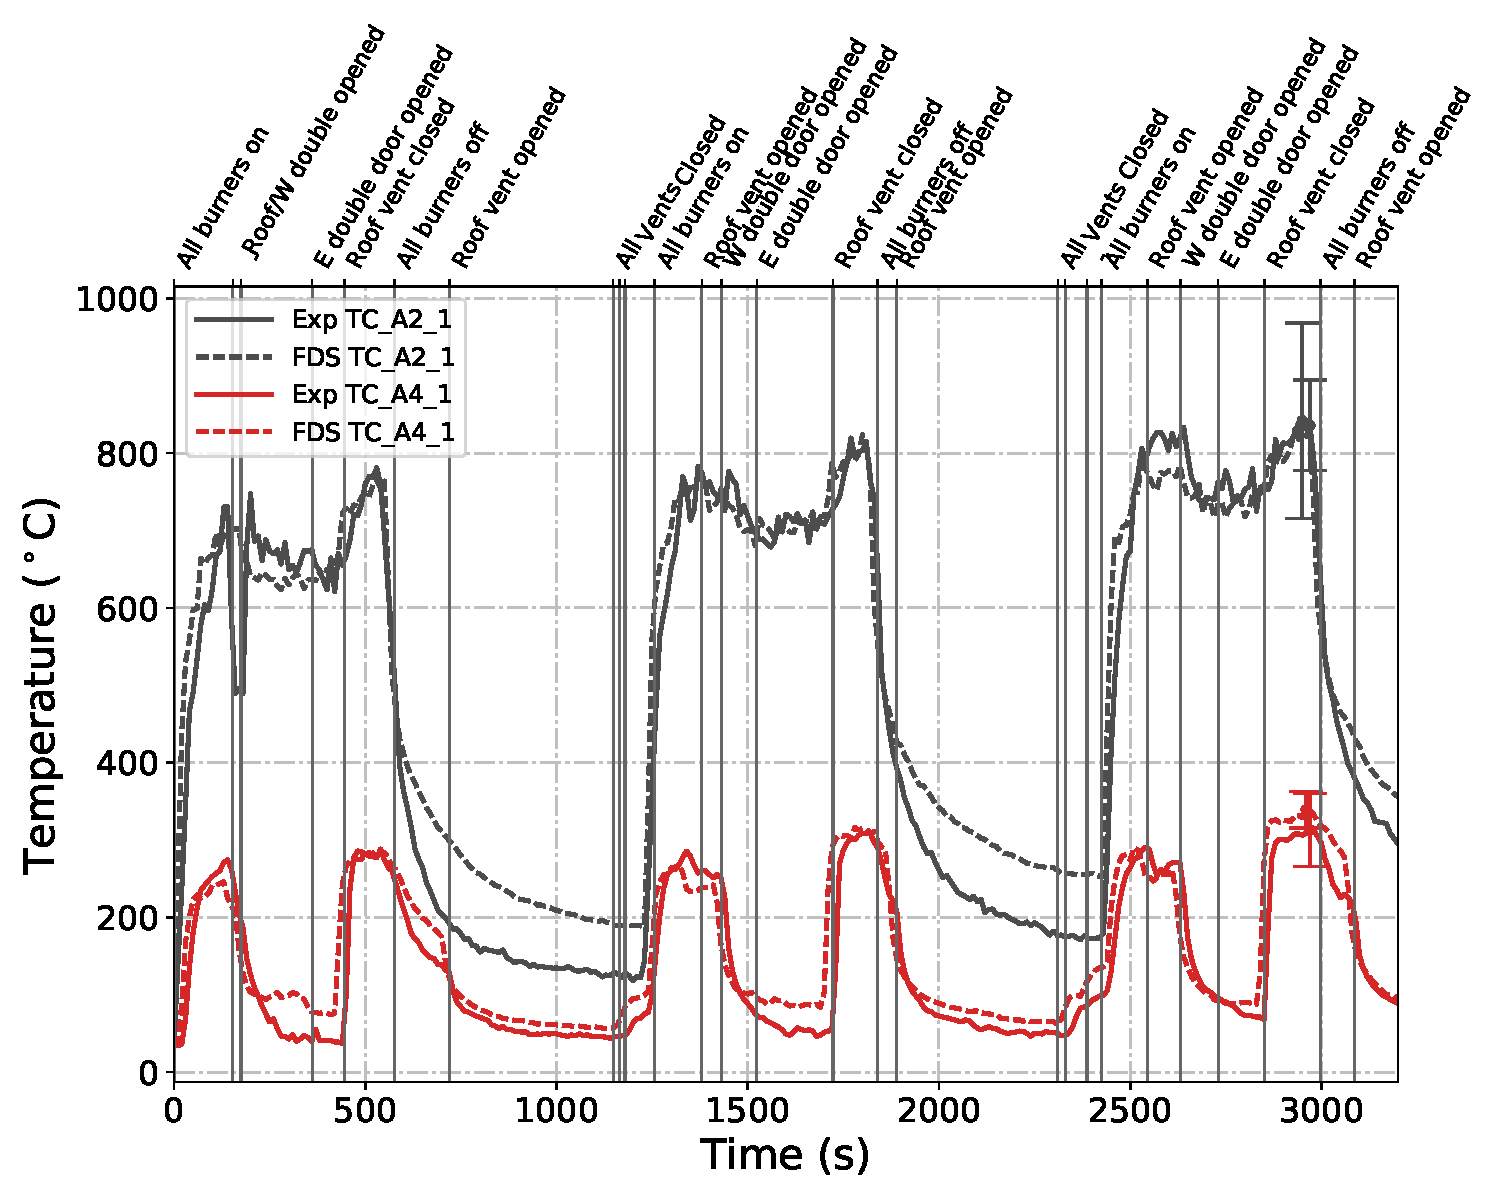
\includegraphics[width=\columnwidth]{../../Plots/Validation/Temperature/Test_5_cjet_2}
	\caption[Plots of measured and predicted ceiling jet temperatures during Test~5.]{Plots of measured and predicted ceiling jet temperatures during Test~5 obtained from thermocouple arrays A2 and A4 located in the fire room and north room of the East Structure, respectively.}
	\label{fig:cjet2_data_Test5}
\end{figure}

\begin{figure}[!h]
	\centering
	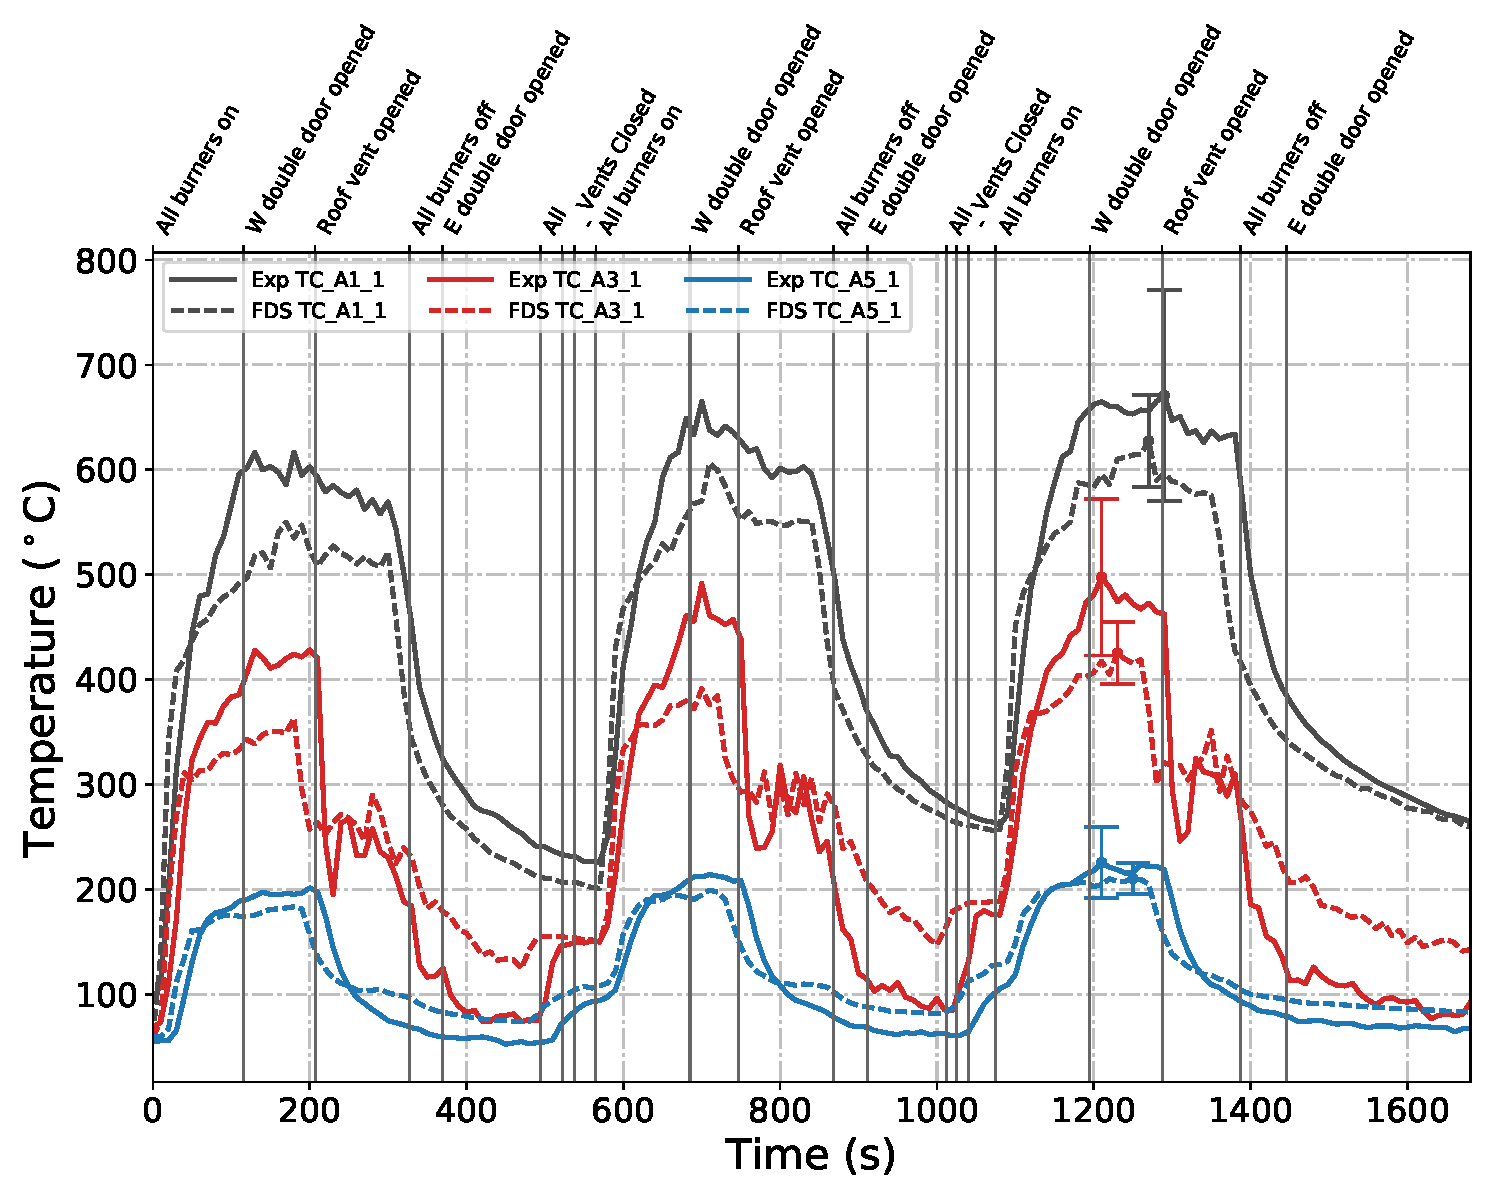
\includegraphics[width=\columnwidth]{../../Plots/Validation/Temperature/Test_6_cjet_1}
	\caption[Plots of measured and predicted ceiling jet temperatures during Test~6.]{Plots of measured and predicted ceiling jet temperatures during Test~6 obtained from thermocouple arrays A1, A3, and A5 located in the fire room, middle room, and north room of the East Structure, respectively.}
	\label{fig:cjet1_data_Test6}
\end{figure}

\begin{figure}[!h]
	\centering
	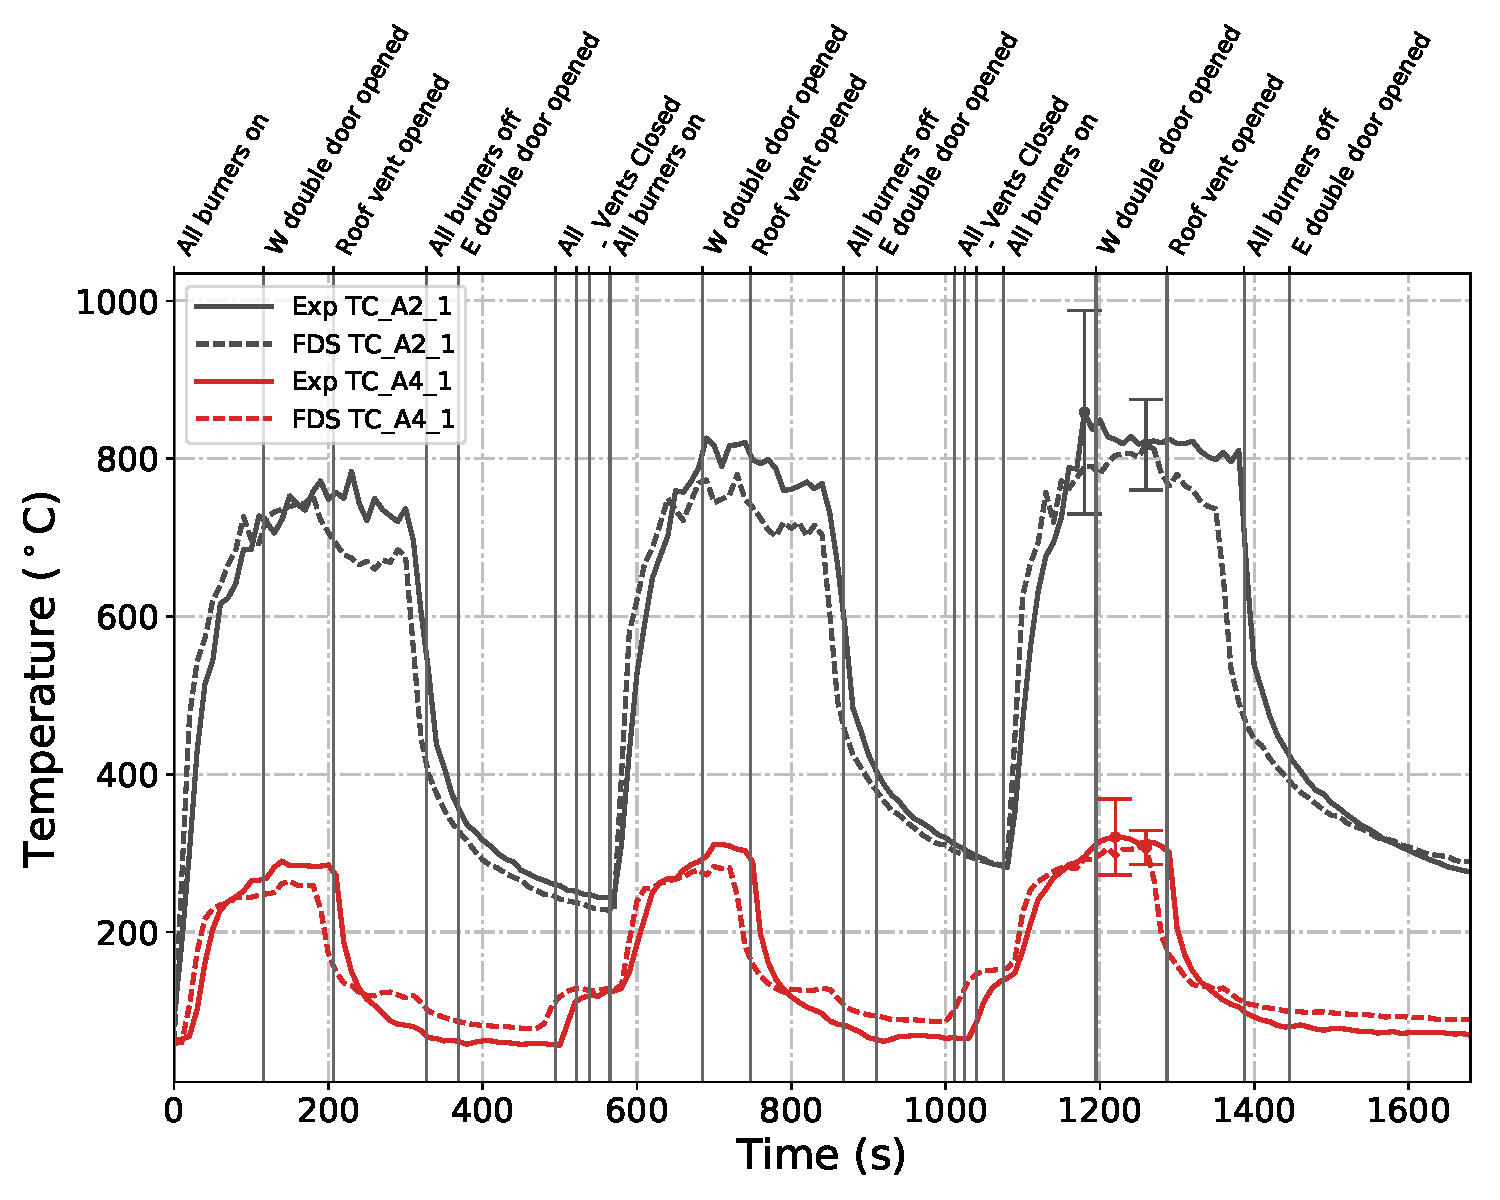
\includegraphics[width=\columnwidth]{../../Plots/Validation/Temperature/Test_6_cjet_2}
	\caption[Plots of measured and predicted ceiling jet temperatures during Test~6.]{Plots of measured and predicted ceiling jet temperatures during Test~6 obtained from thermocouple arrays A2 and A4 located in the fire room and north room of the East Structure, respectively.}
	\label{fig:cjet2_data_Test6}
\end{figure}

\begin{figure}[!h]
	\centering
	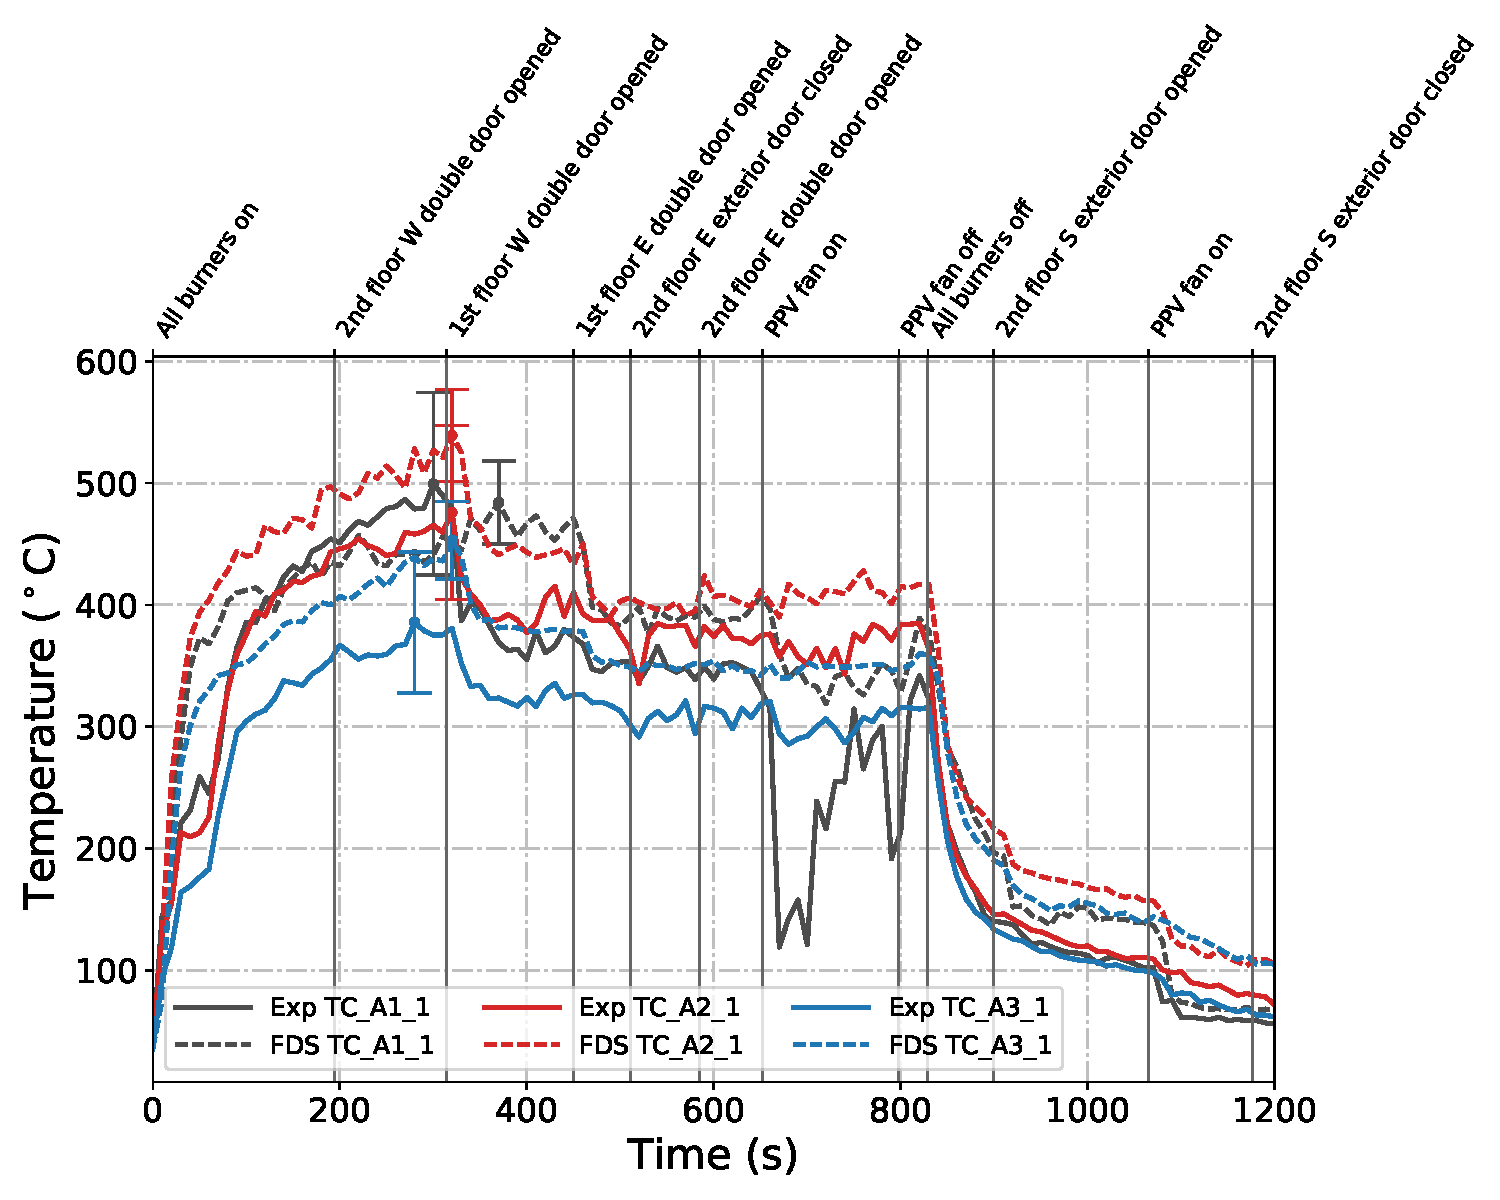
\includegraphics[width=\columnwidth]{../../Plots/Validation/Temperature/Test_22_cjet_1}
	\caption[Plots of measured and predicted ceiling jet temperatures on the first floor during Test~22.]{Plots of measured and predicted ceiling jet temperatures on the first floor of the West Structure during Test~22.}
	\label{fig:cjet1_data_Test22}
\end{figure}

\begin{figure}[!h]
	\centering
	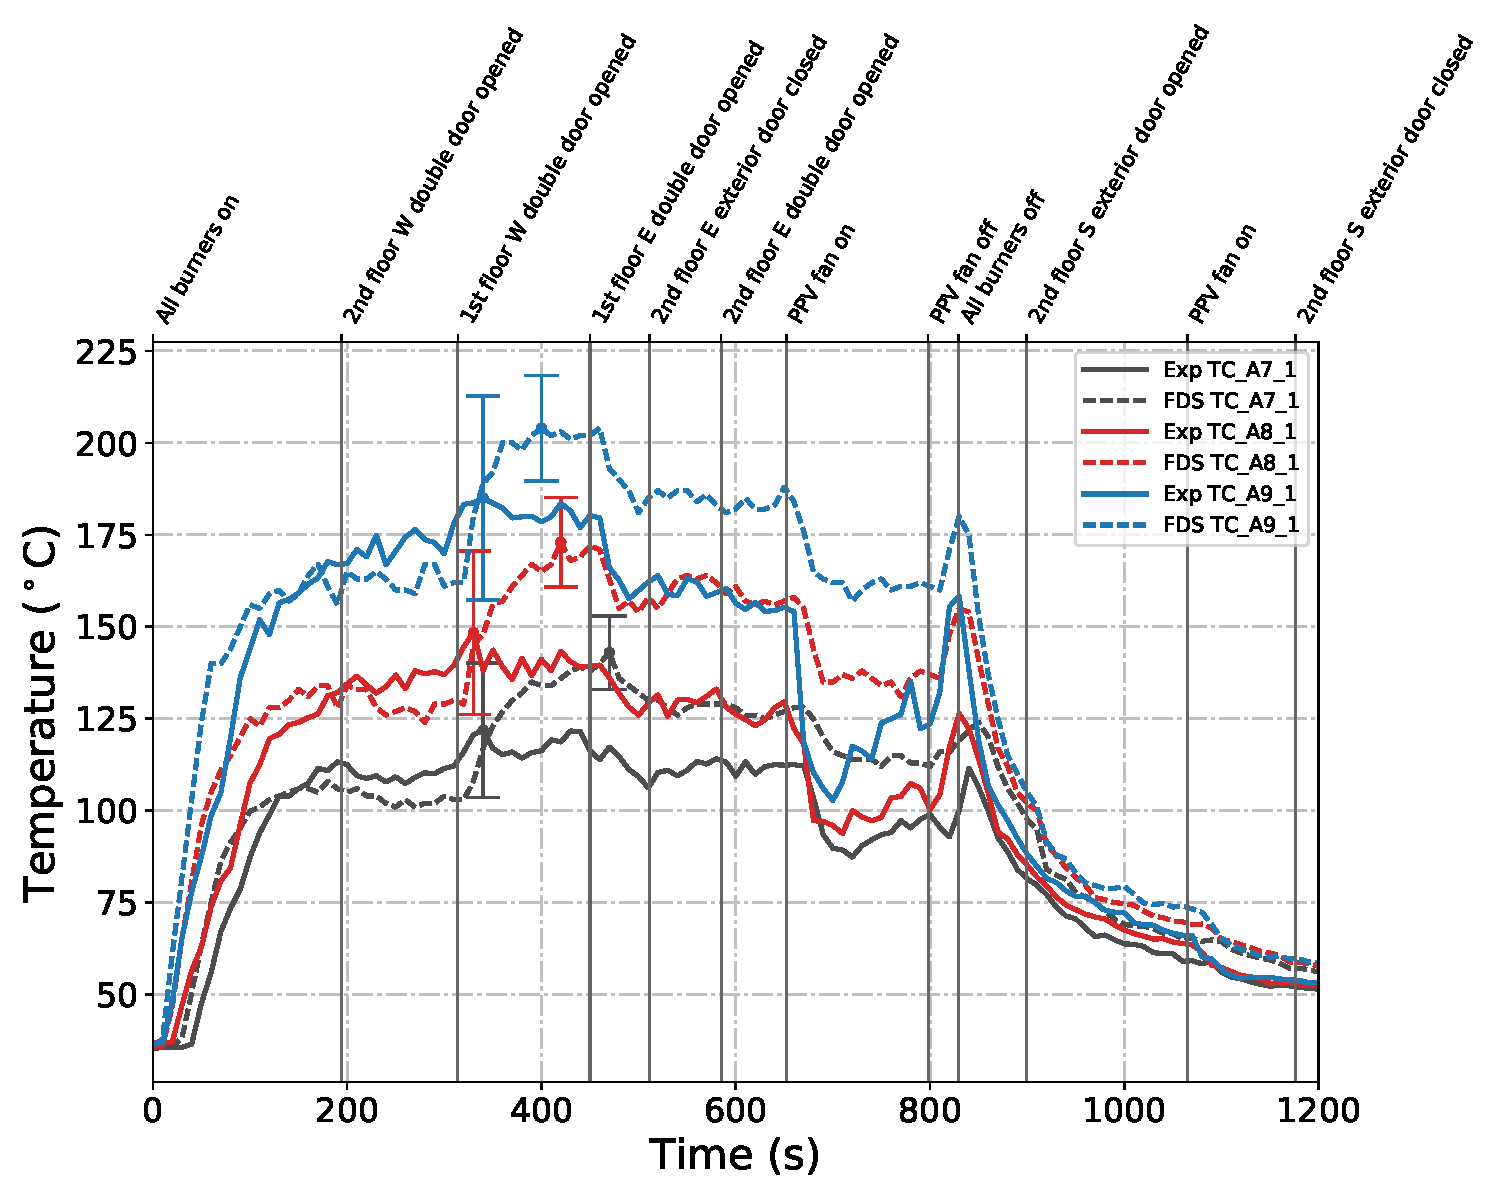
\includegraphics[width=\columnwidth]{../../Plots/Validation/Temperature/Test_22_cjet_2}
	\caption[Plots of measured and predicted ceiling jet temperatures on the second floor during Test~22.]{Plots of measured and predicted ceiling jet temperatures on the second floor of the West Structure during Test~22.}
	\label{fig:cjet2_data_Test22}
\end{figure}

\begin{figure}[!h]
	\centering
	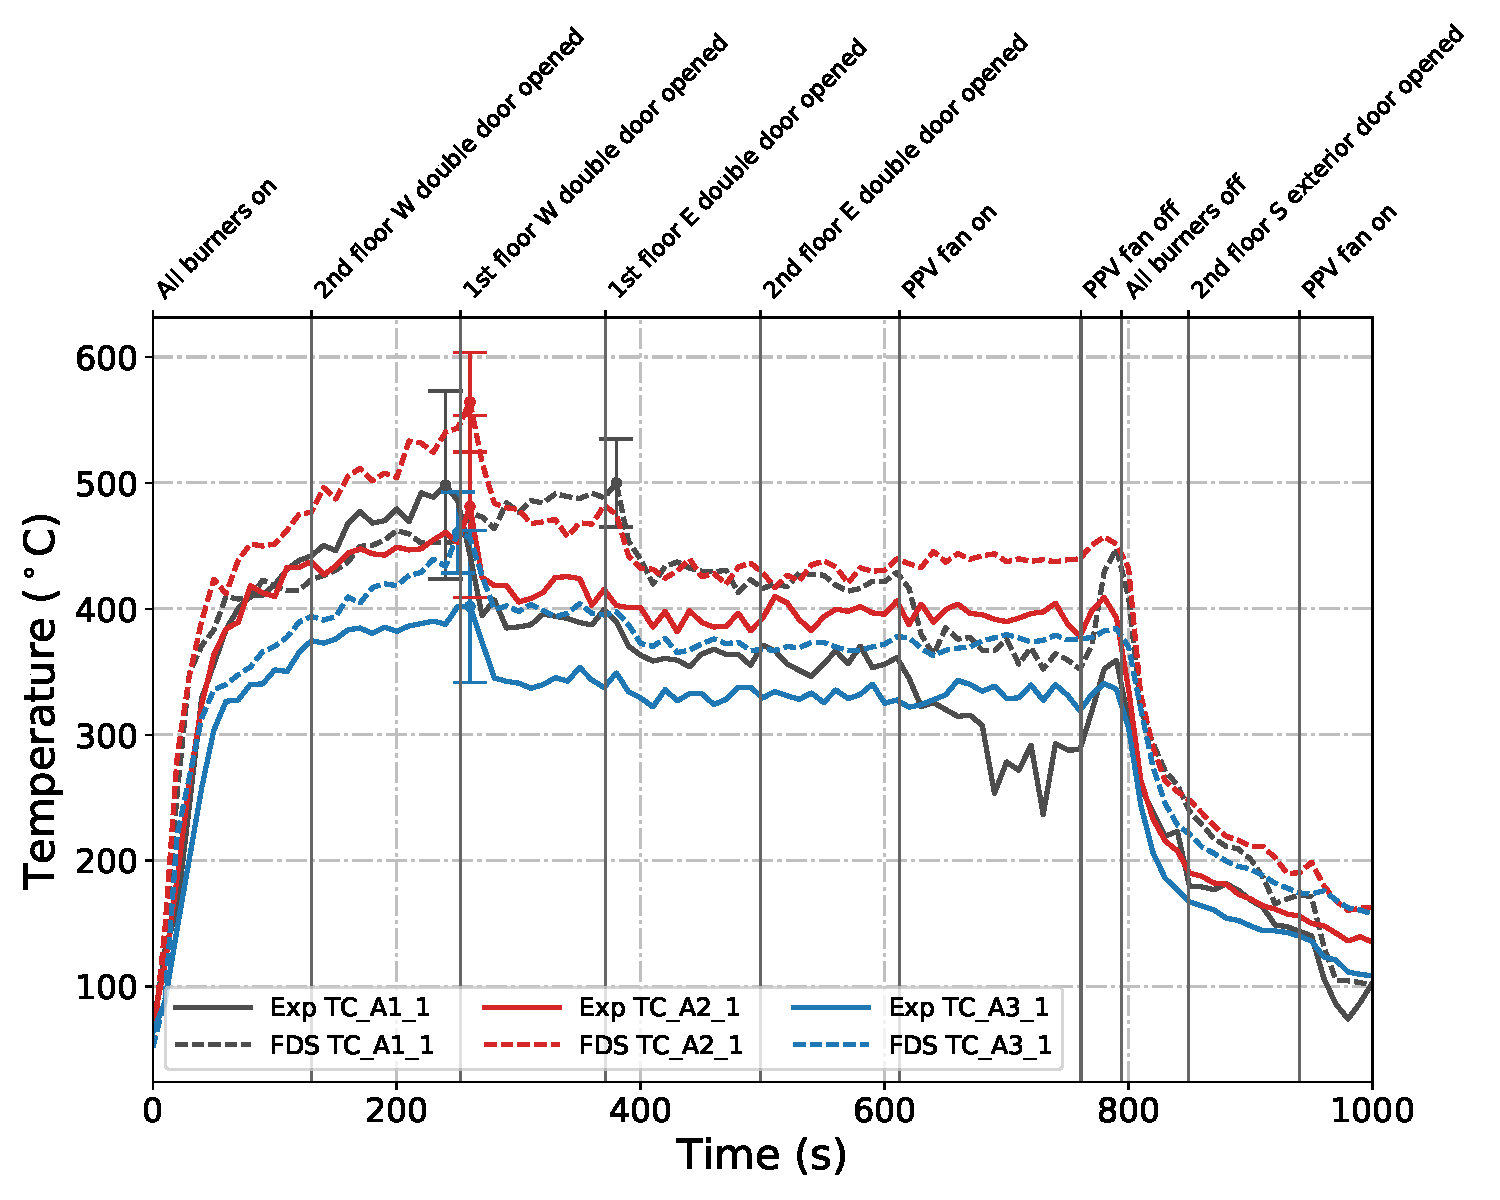
\includegraphics[width=\columnwidth]{../../Plots/Validation/Temperature/Test_23_cjet_1}
	\caption[Plots of measured and predicted ceiling jet temperatures on the first floor during Test~23.]{Plots of measured and predicted ceiling jet temperatures on the first floor of the West Structure during Test~23.}
	\label{fig:cjet1_data_Test23}
\end{figure}

\begin{figure}[!h]
	\centering
	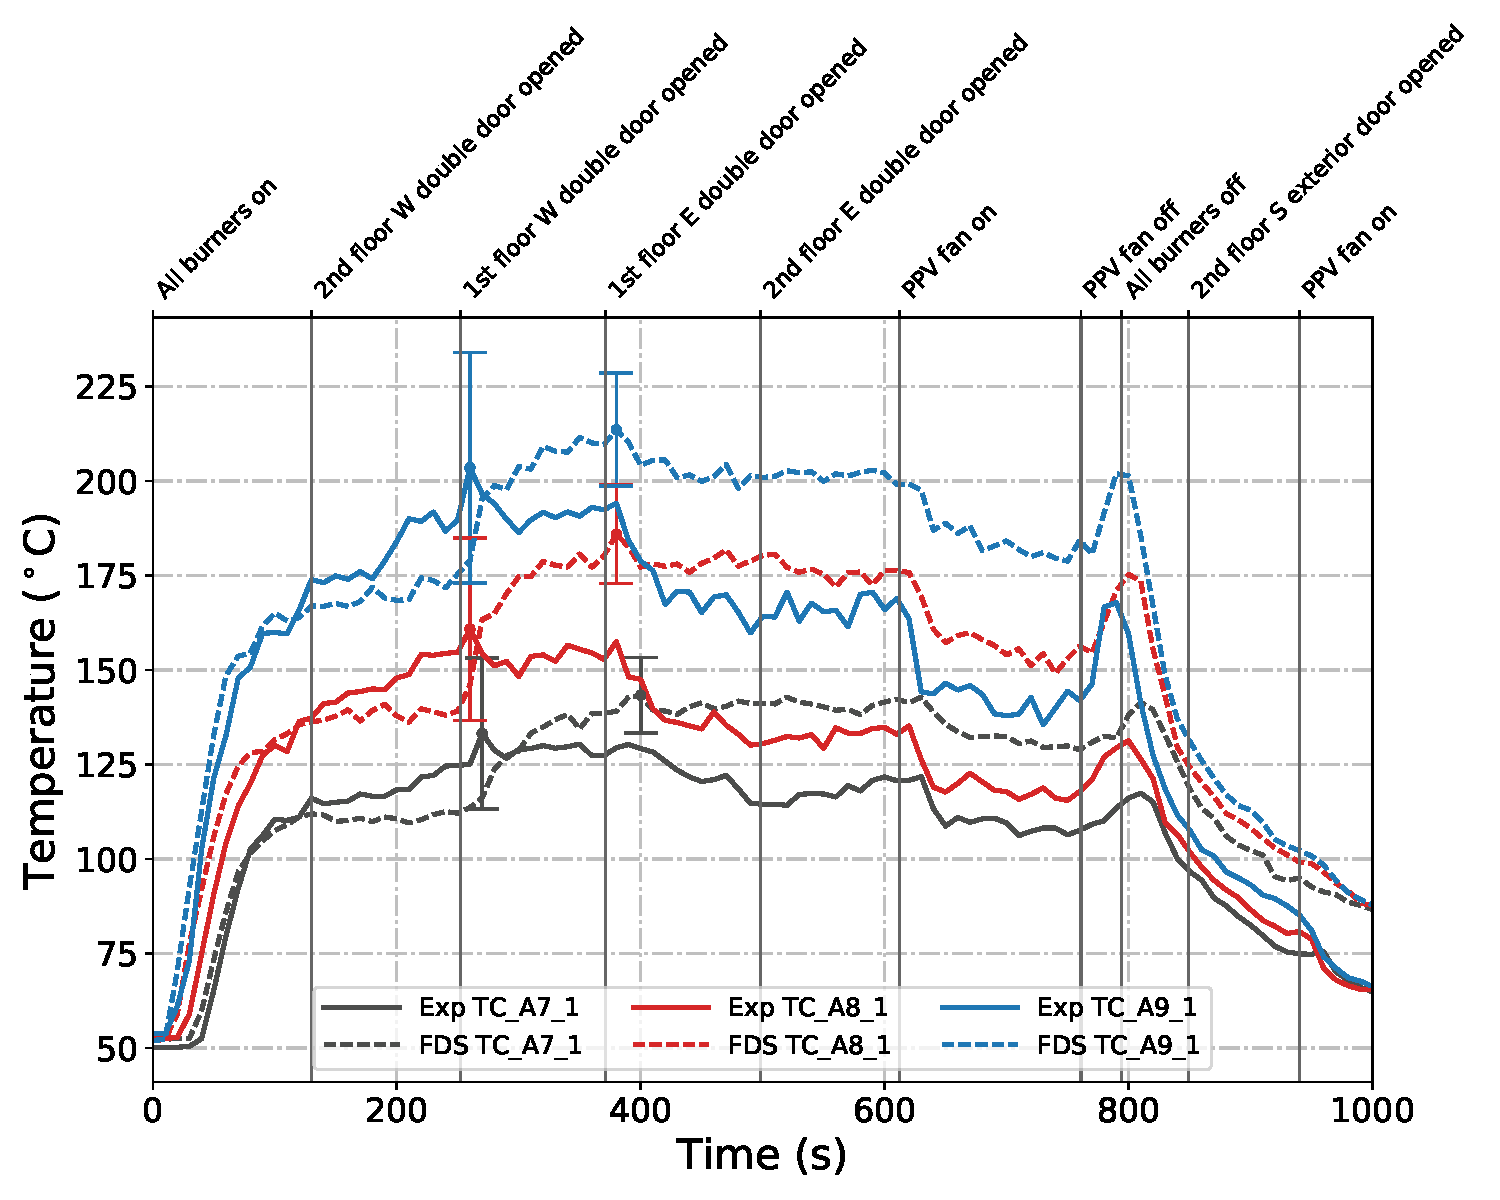
\includegraphics[width=\columnwidth]{../../Plots/Validation/Temperature/Test_23_cjet_2}
	\caption[Plots of measured and predicted ceiling jet temperatures on the second floor during Test~23.]{Plots of measured and predicted ceiling jet temperatures on the second floor of the West Structure during Test~23.}
	\label{fig:cjet2_data_Test23}
\end{figure}

\begin{figure}[!h]
	\centering
	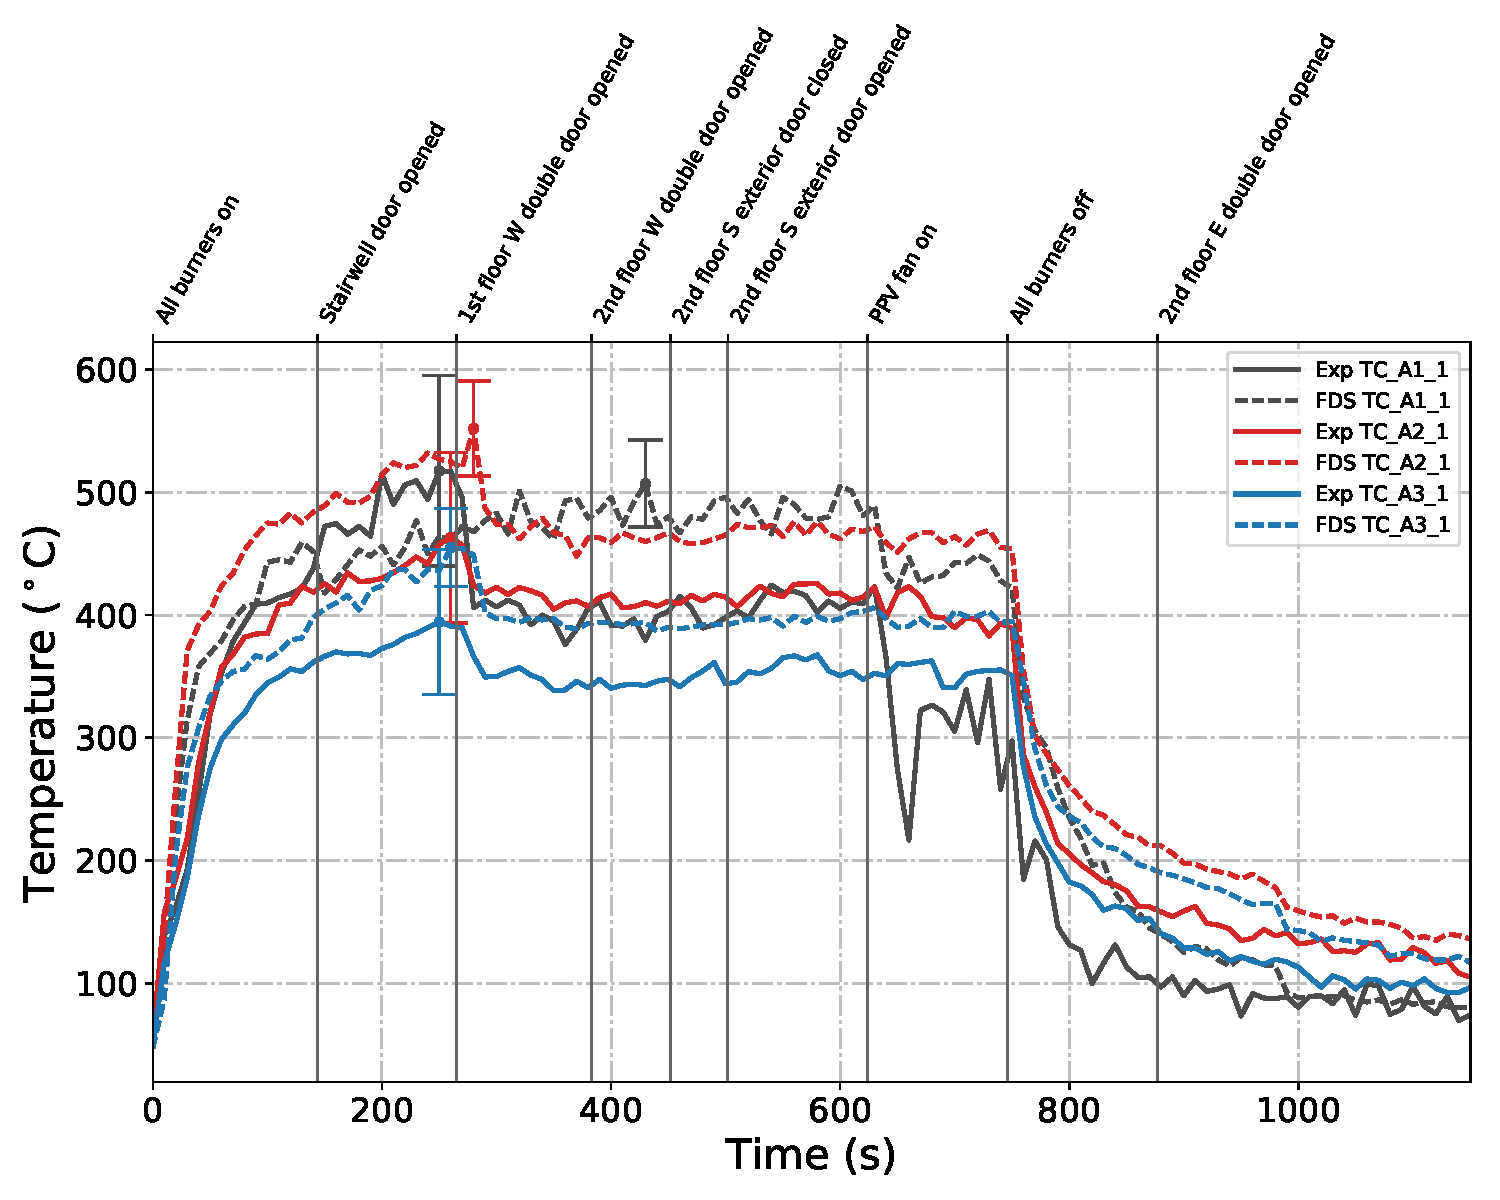
\includegraphics[width=\columnwidth]{../../Plots/Validation/Temperature/Test_24_cjet_1}
	\caption[Plots of measured and predicted ceiling jet temperatures on the first floor during Test~24.]{Plots of measured and predicted ceiling jet temperatures on the first floor of the West Structure during Test~24.}
	\label{fig:cjet1_data_Test24}
\end{figure}

\begin{figure}[!h]
	\centering
	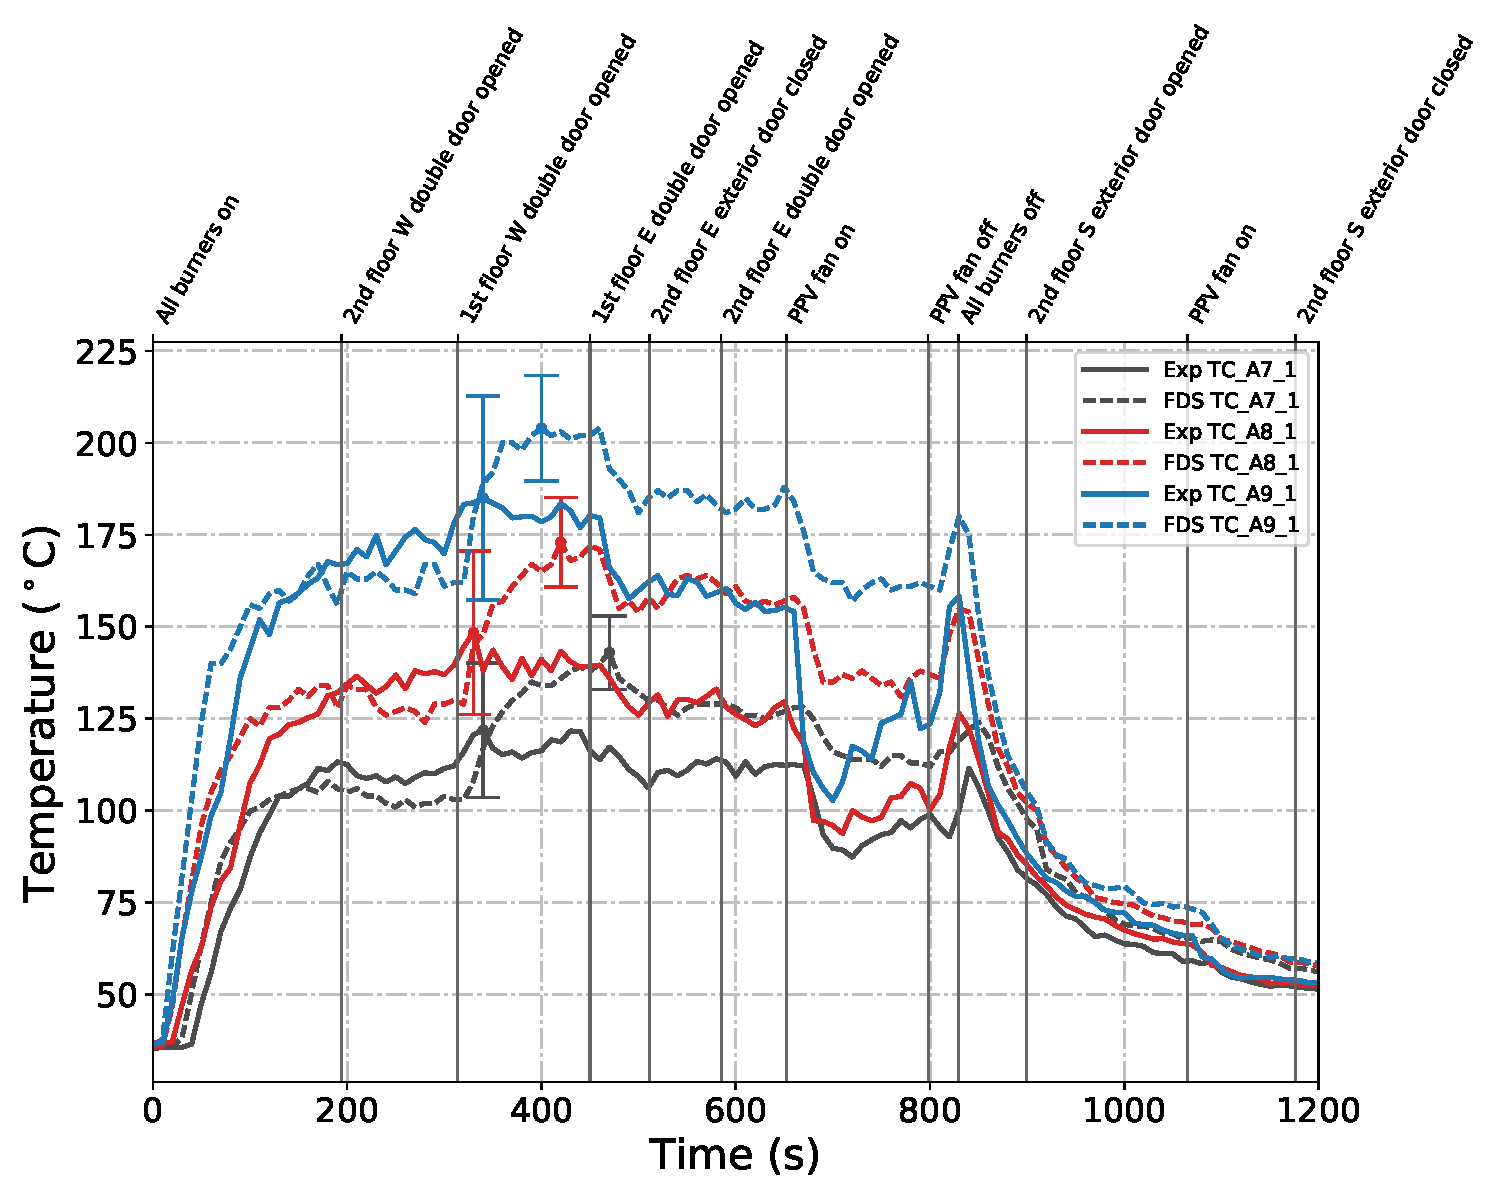
\includegraphics[width=\columnwidth]{../../Plots/Validation/Temperature/Test_22_cjet_2}
	\caption[Plots of measured and predicted ceiling jet temperatures on the second floor during Test~24.]{Plots of measured and predicted ceiling jet temperatures on the second floor of the West Structure during Test~24.}
	\label{fig:cjet2_data_Test24}
\end{figure}

\begin{figure}[!h]
	\centering
	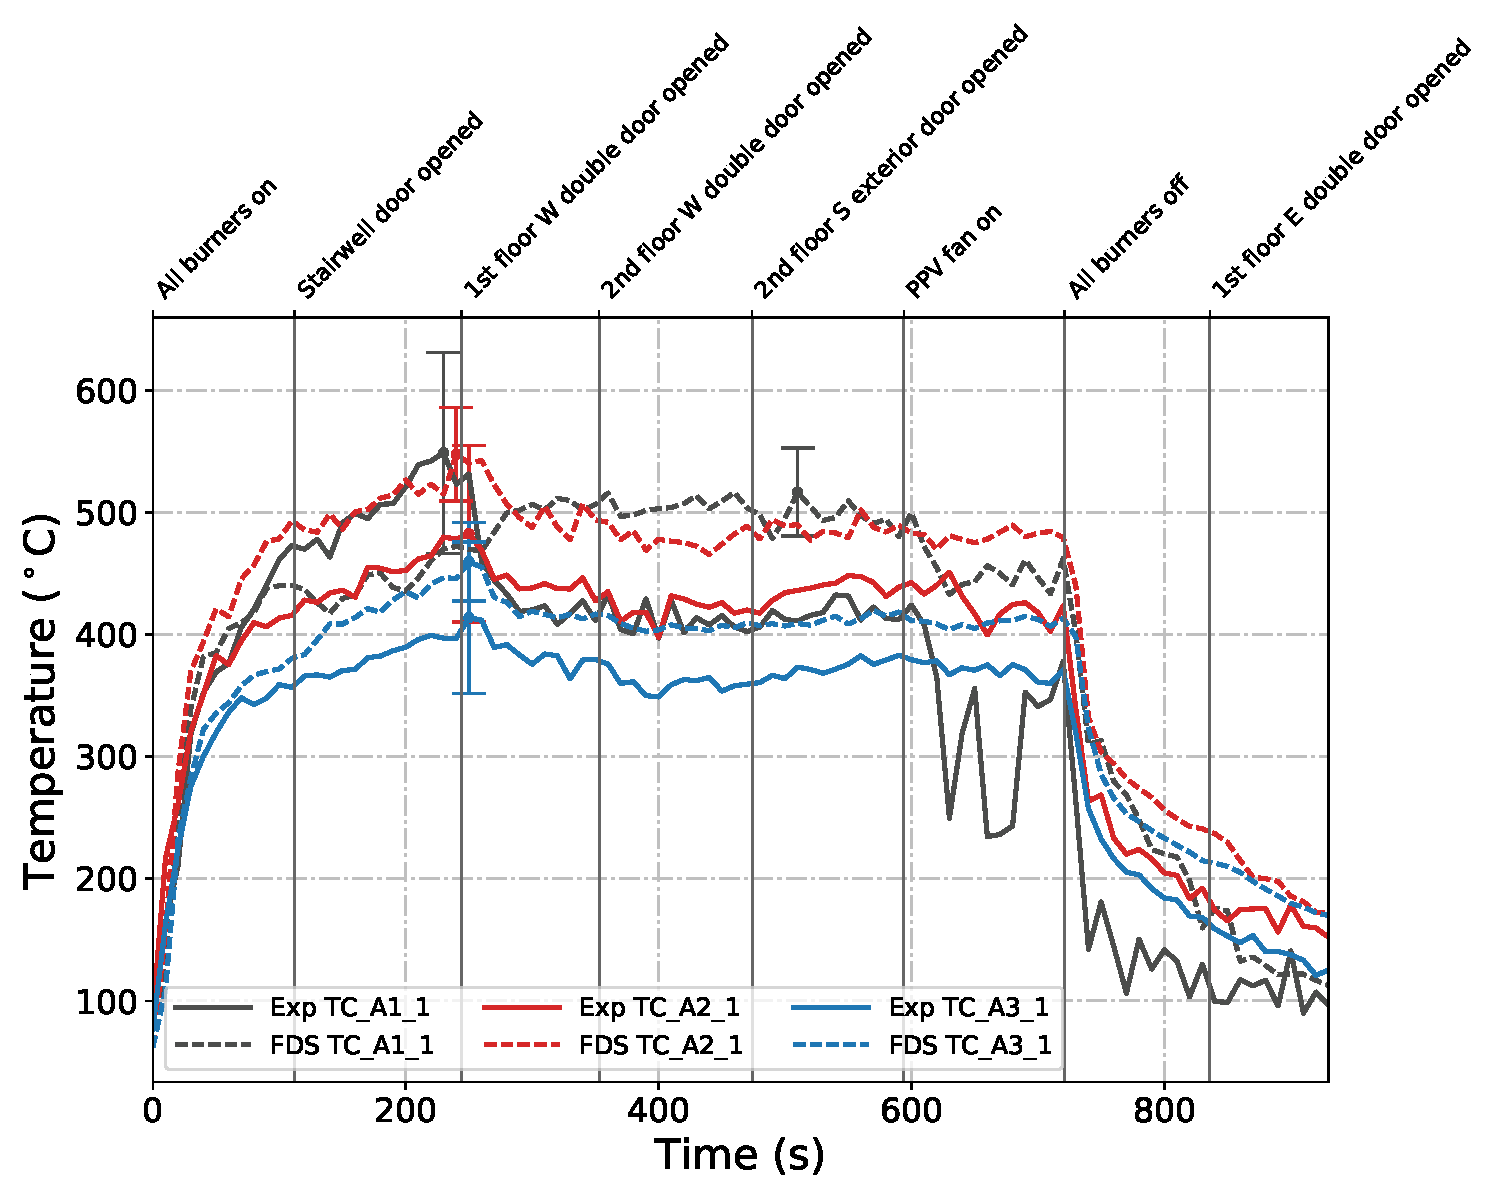
\includegraphics[width=\columnwidth]{../../Plots/Validation/Temperature/Test_25_cjet_1}
	\caption[Plots of measured and predicted ceiling jet temperatures on the first floor during Test~25.]{Plots of measured and predicted ceiling jet temperatures on the first floor of the West Structure during Test~25.}
	\label{fig:cjet1_data_Test25}
\end{figure}

\begin{figure}[!h]
	\centering
	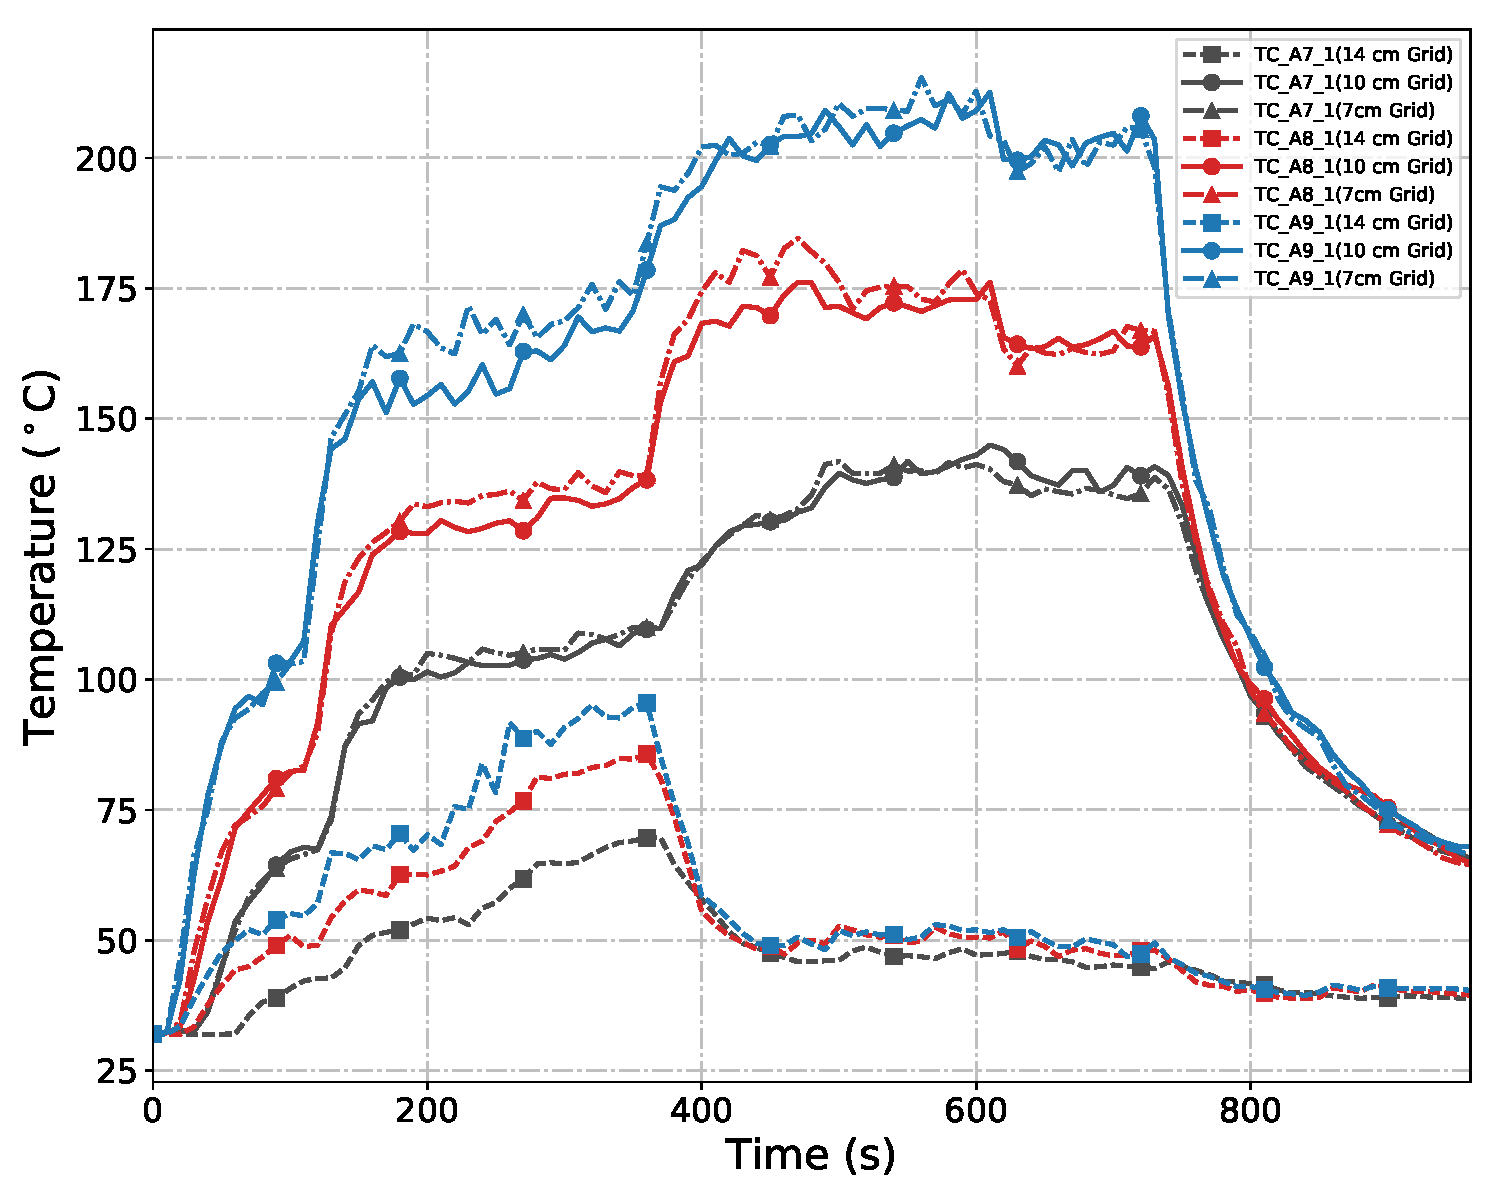
\includegraphics[width=\columnwidth]{../../Plots/Validation/Temperature/Test_25_cjet_2}
	\caption[Plots of measured and predicted ceiling jet temperatures on the second floor during Test~25.]{Plots of measured and predicted ceiling jet temperatures on the second floor of the West Structure during Test~25.}
	\label{fig:cjet2_data_Test25}
\end{figure}

\clearpage
\subsection*{\textit{Thermocouple Array Temperatures}}
\begin{figure}[!h]
	\centering
	\includegraphics[width=\columnwidth]{../../Plots/Validation/Temperature/Test_24_TC_A1}
	\caption[Plots of measured and predicted thermocouple array temperatures during Test~24.]{Plots of measured and predicted temperatures during Test~24 obtained from thermocouple array A1.}
	\label{fig:TCarray_data}
\end{figure}

\clearpage
\section{Gas Species Concentration}
\subsection*{\textit{O$_2$ Concentration}}
\begin{figure}[!h]
	\centering
	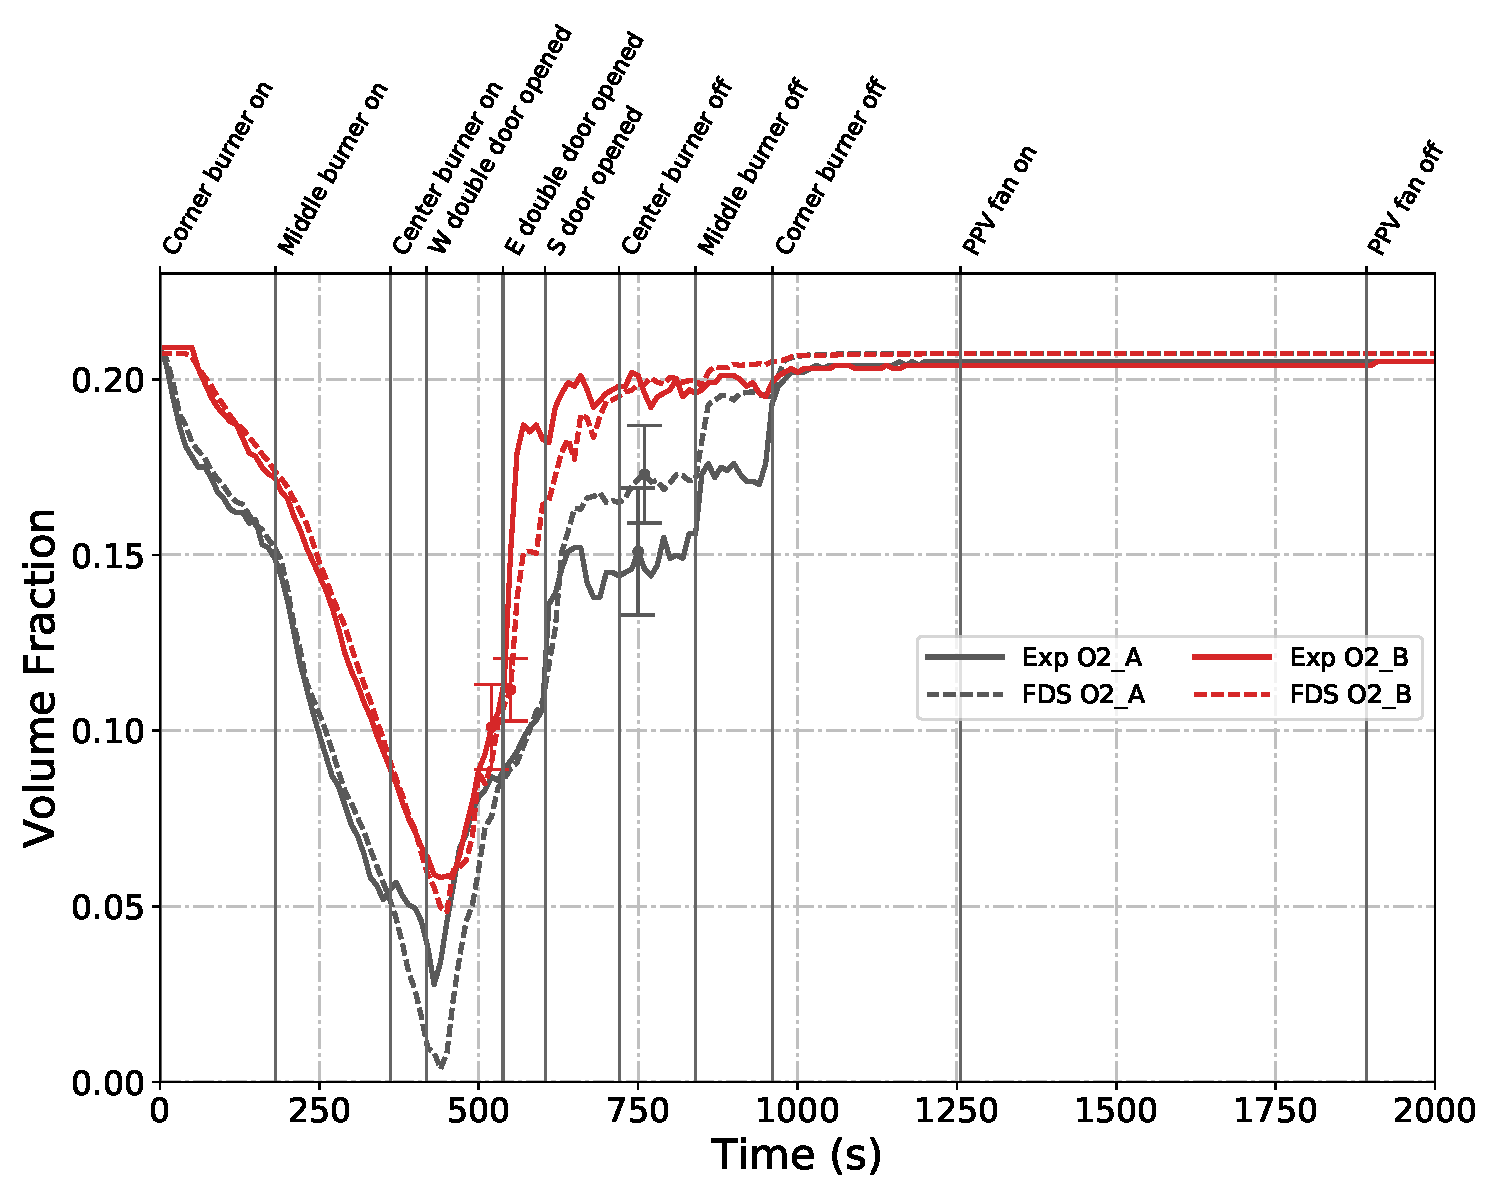
\includegraphics[width=\columnwidth]{../../Plots/Validation/Gas_Concentration/Test_2_O2}
	\caption[Plots of measured and predicted $O_2$ concentration during Test~2.]{Plots of measured and predicted $O_2$ concentration in the fire room (black plots) and north room (red plots) of the East Structure during Test~2.}
	\label{fig:Test2_O2}
\end{figure}

\begin{figure}[!h]
	\centering
	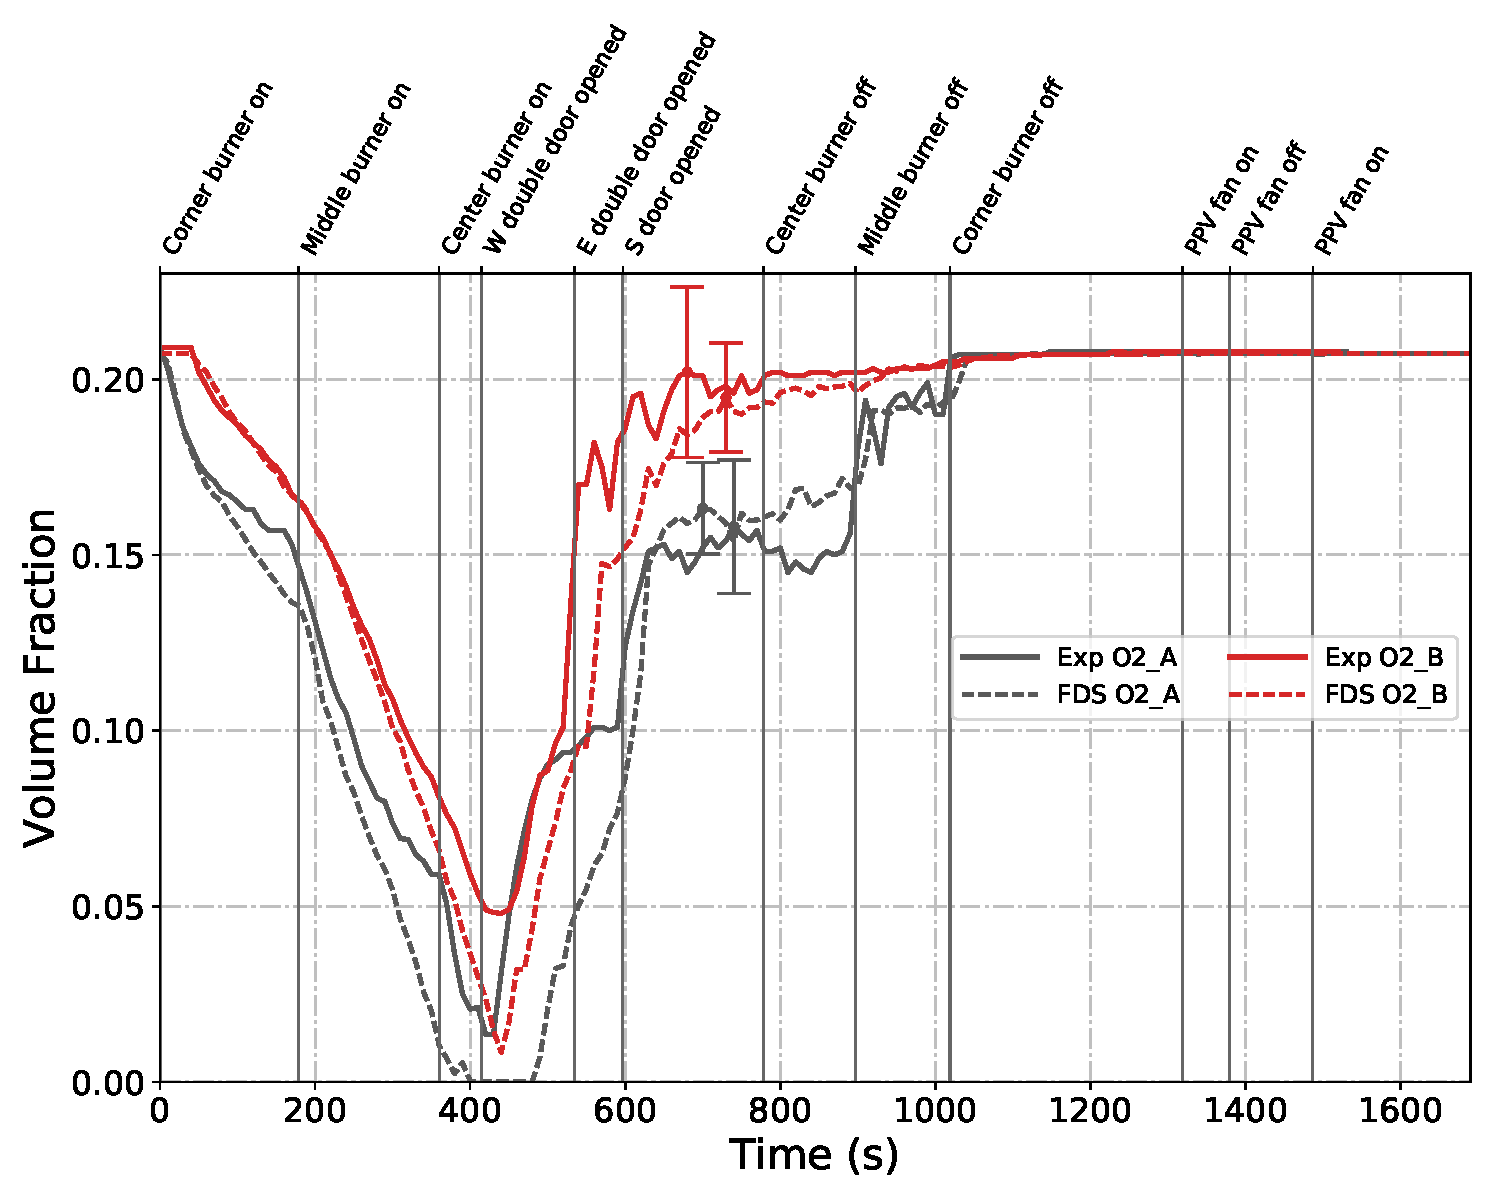
\includegraphics[width=\columnwidth]{../../Plots/Validation/Gas_Concentration/Test_4_O2}
	\caption[Plots of measured and predicted $O_2$ concentration during Test~4.]{Plots of measured and predicted $O_2$ concentration in the fire room (black plots) and north room (red plots) of the East Structure during Test~4.}
	\label{fig:Test4_O2}
\end{figure}

\begin{figure}[!h]
	\centering
	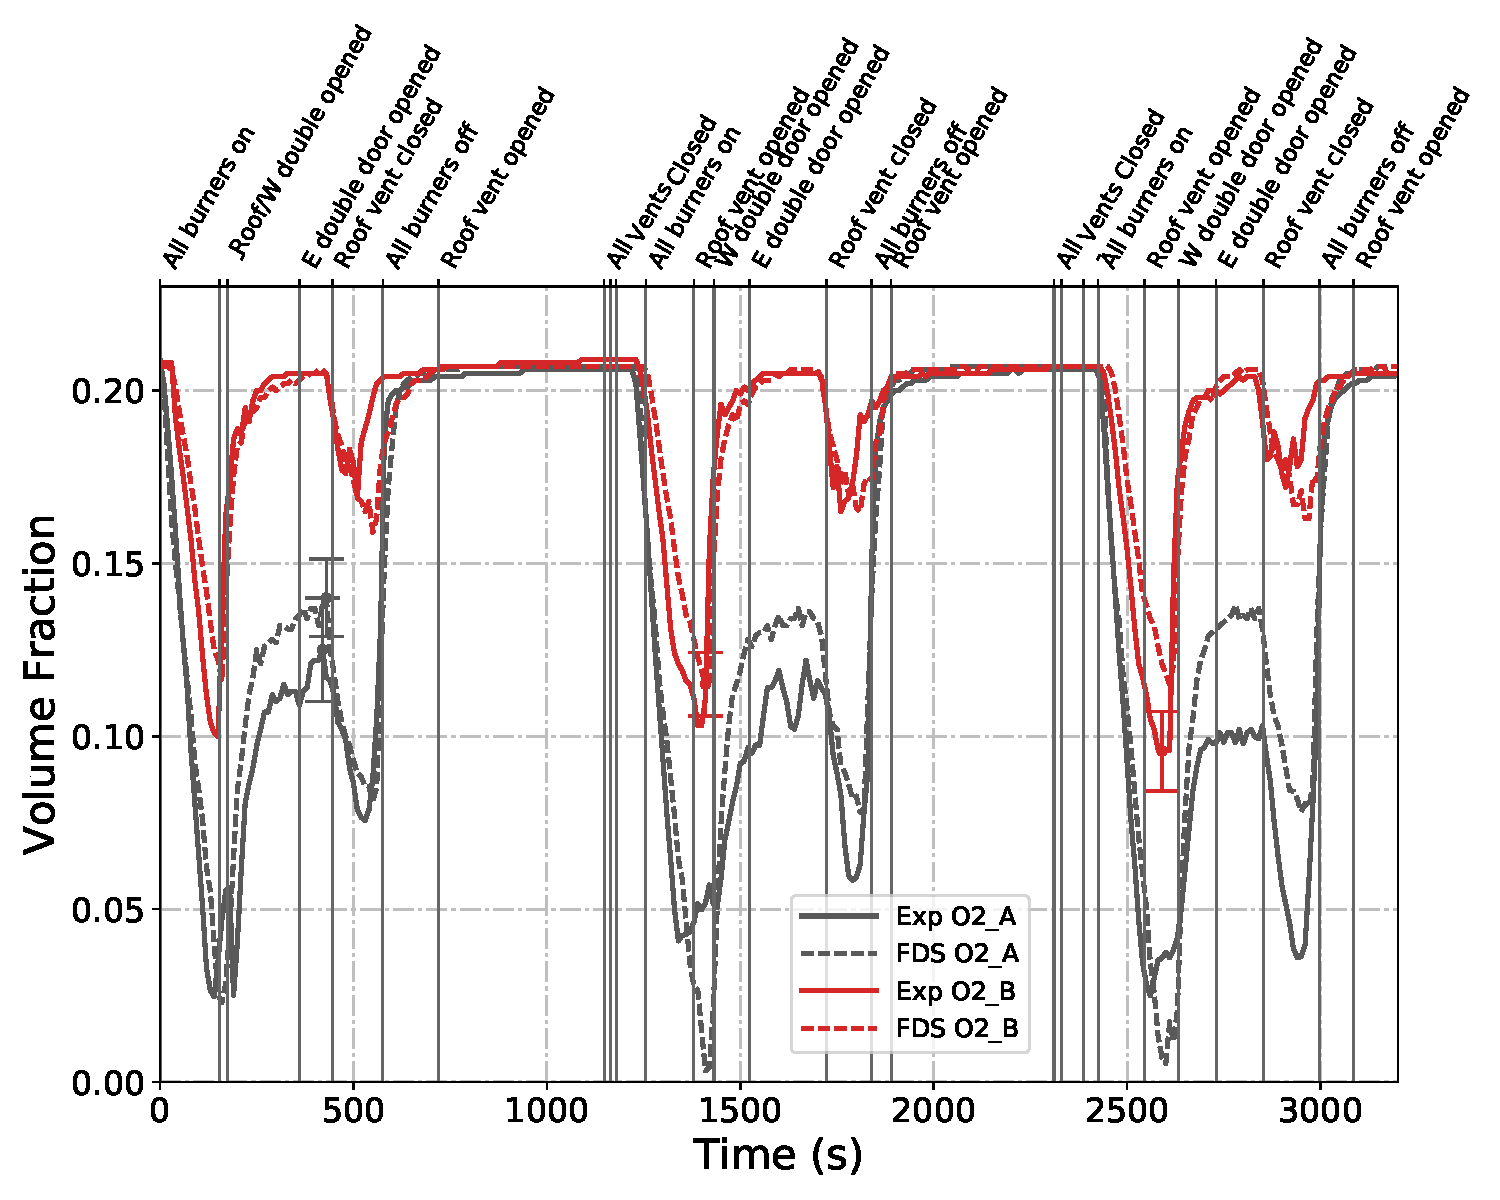
\includegraphics[width=\columnwidth]{../../Plots/Validation/Gas_Concentration/Test_5_O2}
	\caption[Plots of measured and predicted $O_2$ concentration during Test~5.]{Plots of measured and predicted $O_2$ concentration in the fire room (black plots) and north room (red plots) of the East Structure during Test~5.}
	\label{fig:Test5_O2}
\end{figure}

\begin{figure}[!h]
	\centering
	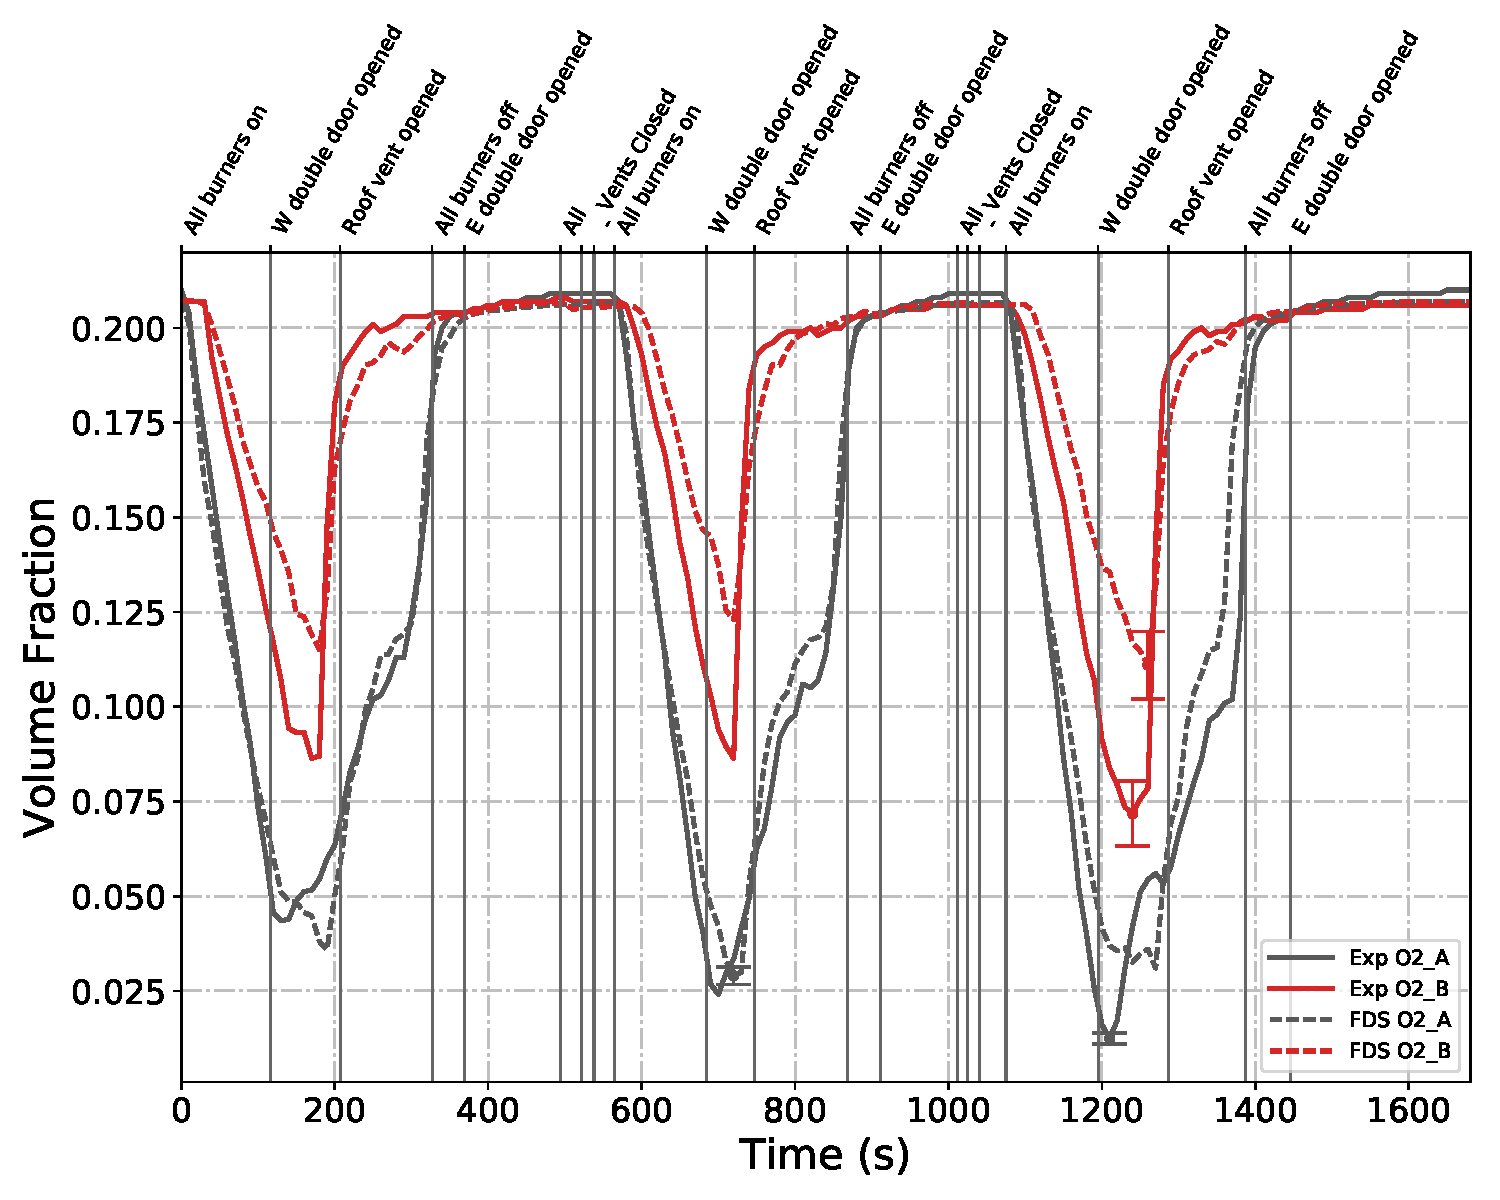
\includegraphics[width=\columnwidth]{../../Plots/Validation/Gas_Concentration/Test_6_O2}
	\caption[Plots of measured and predicted $O_2$ concentration during Test~6.]{Plots of measured and predicted $O_2$ concentration in the fire room (black plots) and north room (red plots) of the East Structure during Test~6.}
	\label{fig:Test6_O2}
\end{figure}

\begin{figure}[!h]
	\centering
	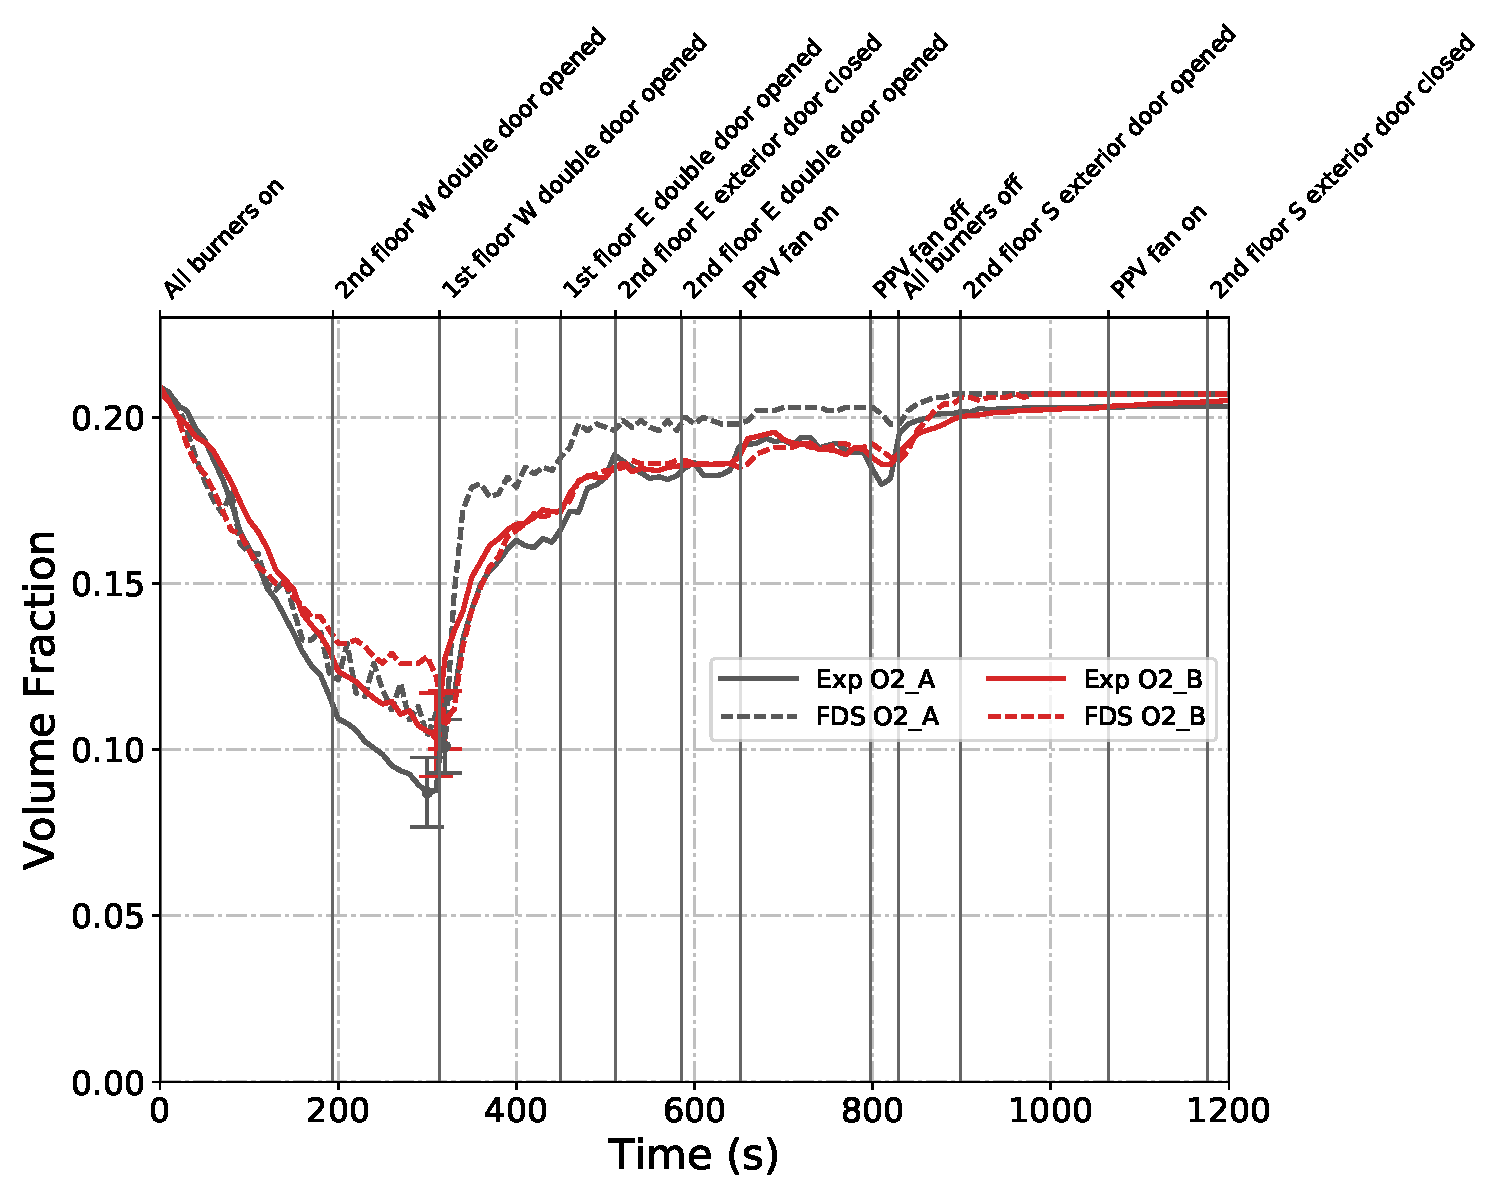
\includegraphics[width=\columnwidth]{../../Plots/Validation/Gas_Concentration/Test_22_O2}
	\caption[Plots of measured and predicted $O_2$ concentration during Test~22.]{Plots of measured and predicted $O_2$ concentration on the first floor (black plots) and second floor (red plots) of the West Structure during Test~22.}
	\label{fig:Test22_O2}
\end{figure}

\begin{figure}[!h]
	\centering
	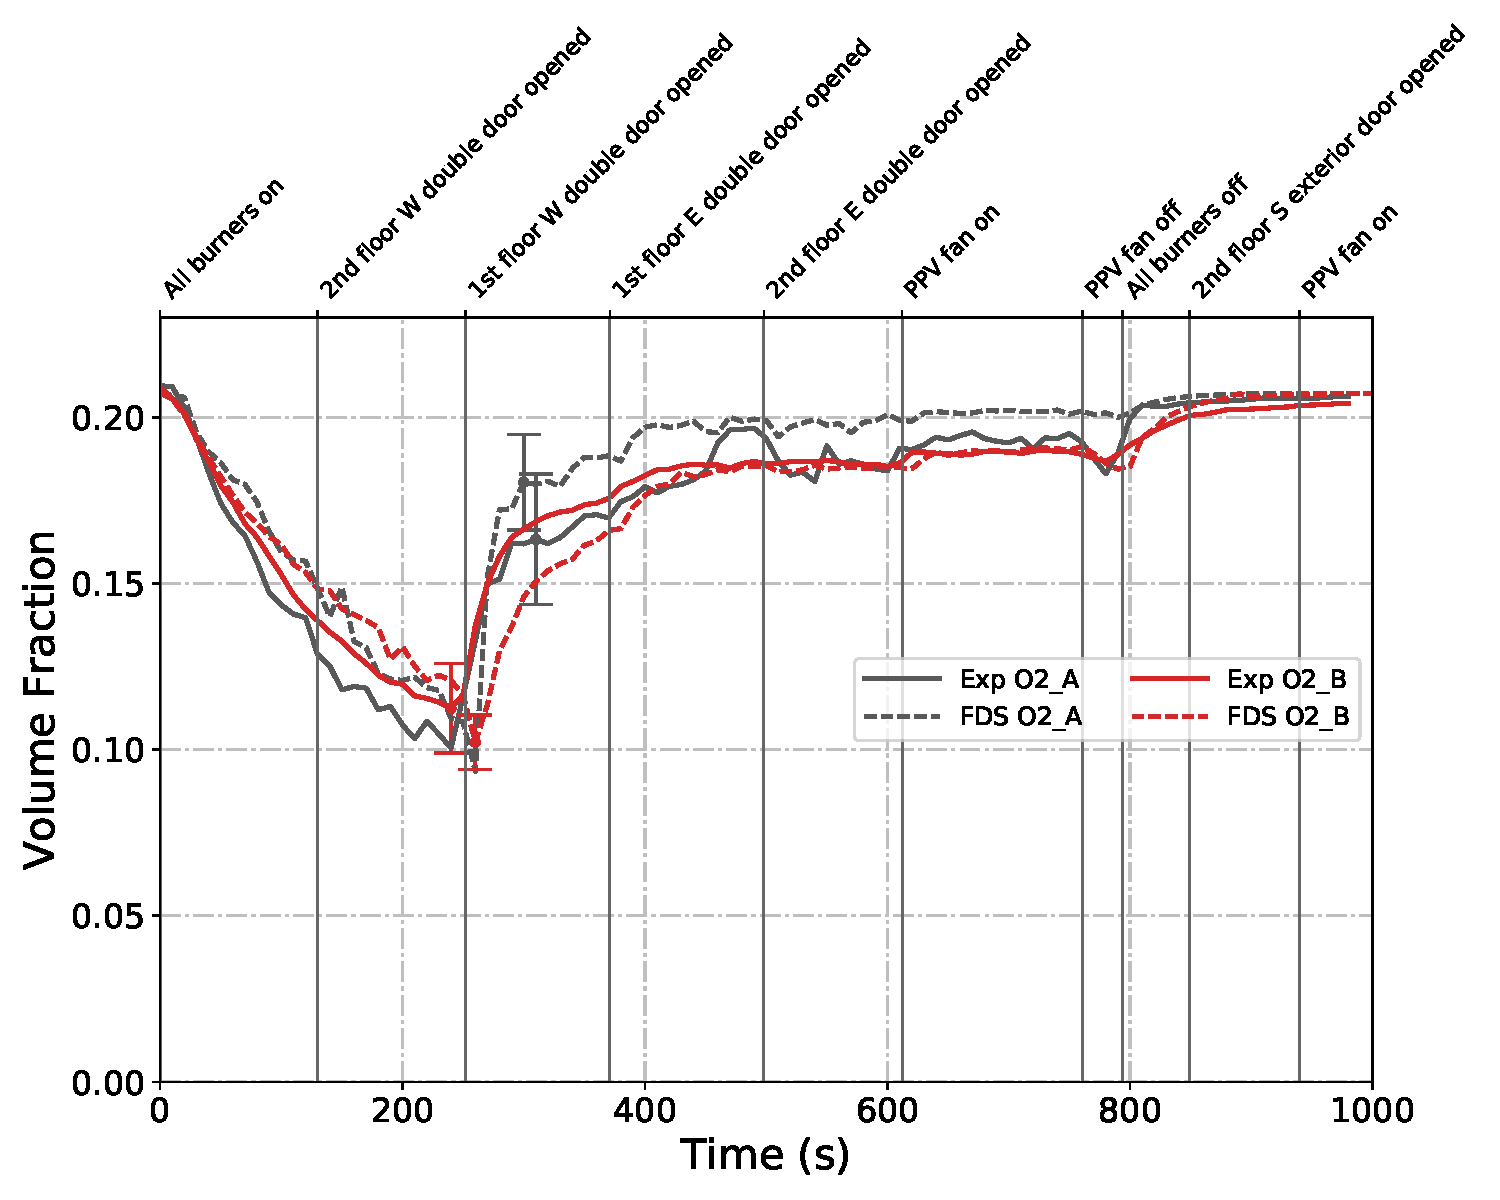
\includegraphics[width=\columnwidth]{../../Plots/Validation/Gas_Concentration/Test_23_O2}
	\caption[Plots of measured and predicted $O_2$ concentration during Test~23.]{Plots of measured and predicted $O_2$ concentration on the first floor (black plots) and second floor (red plots) of the West Structure during Test~23.}
	\label{fig:Test23_O2}
\end{figure}

\begin{figure}[!h]
	\centering
	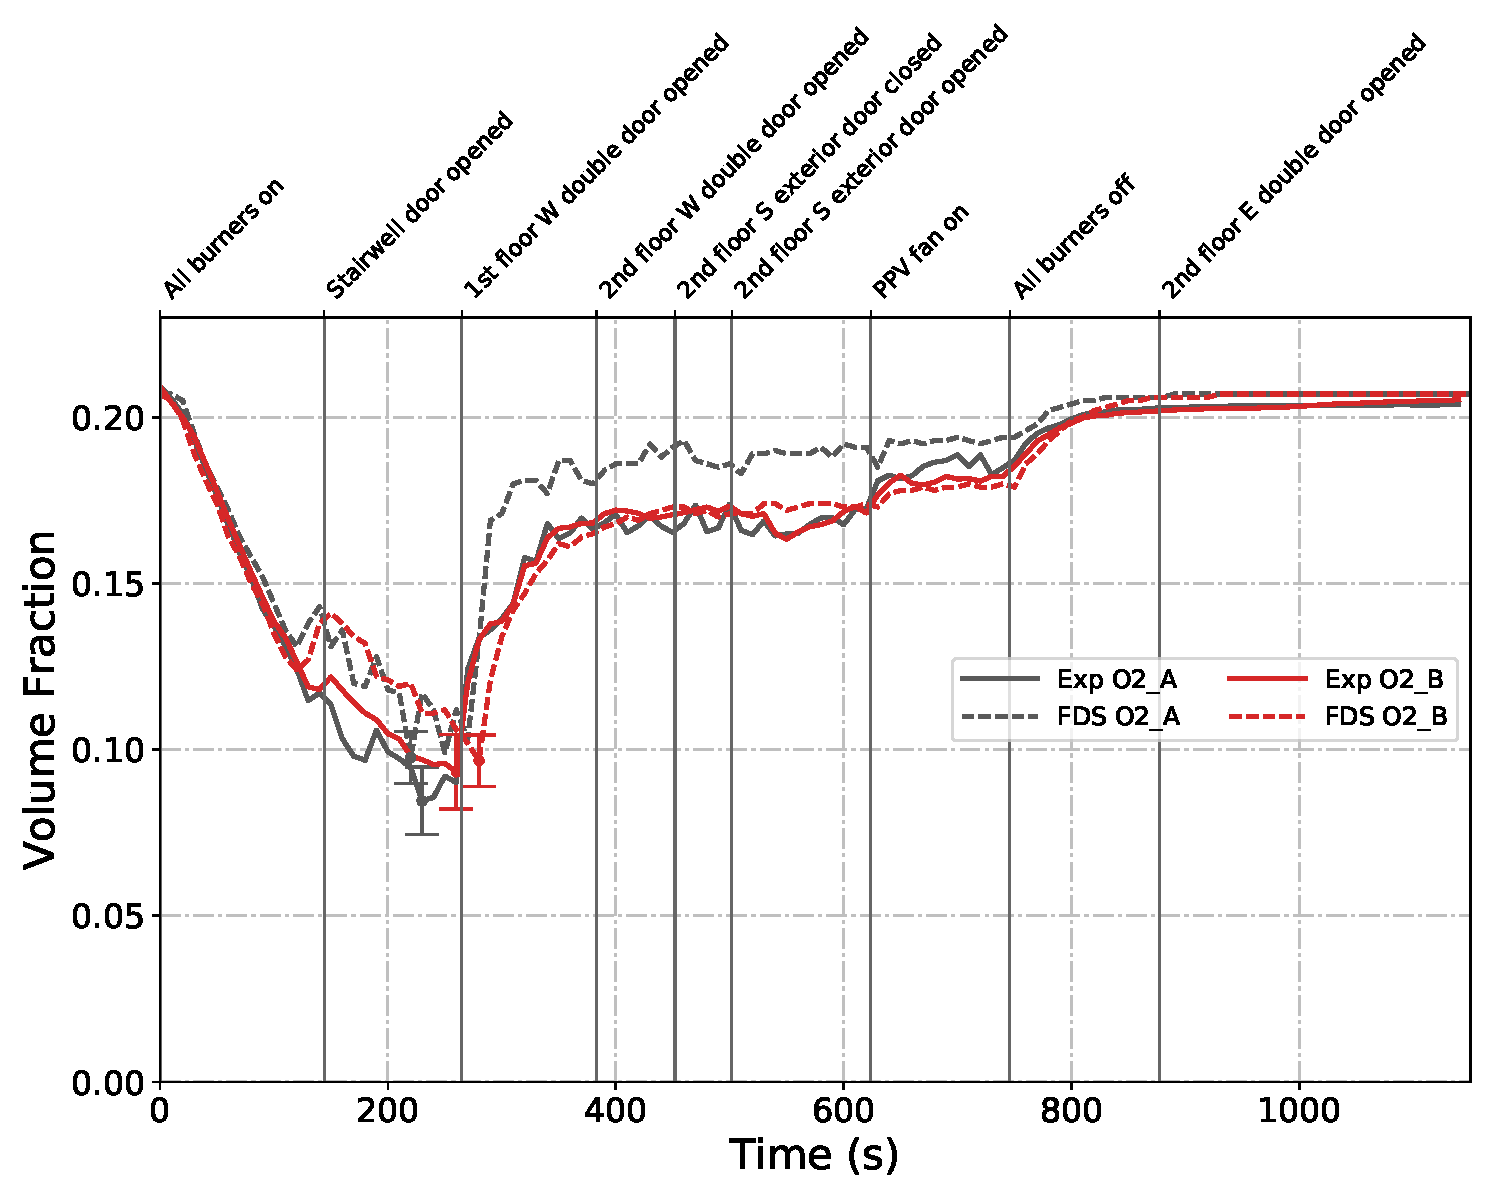
\includegraphics[width=\columnwidth]{../../Plots/Validation/Gas_Concentration/Test_24_O2}
	\caption[Plots of measured and predicted $O_2$ concentration during Test~24.]{Plots of measured and predicted $O_2$ concentration on the first floor (black plots) and second floor (red plots) of the West Structure during Test~24.}
	\label{fig:Test24_O2}
\end{figure}

\begin{figure}[!h]
	\centering
	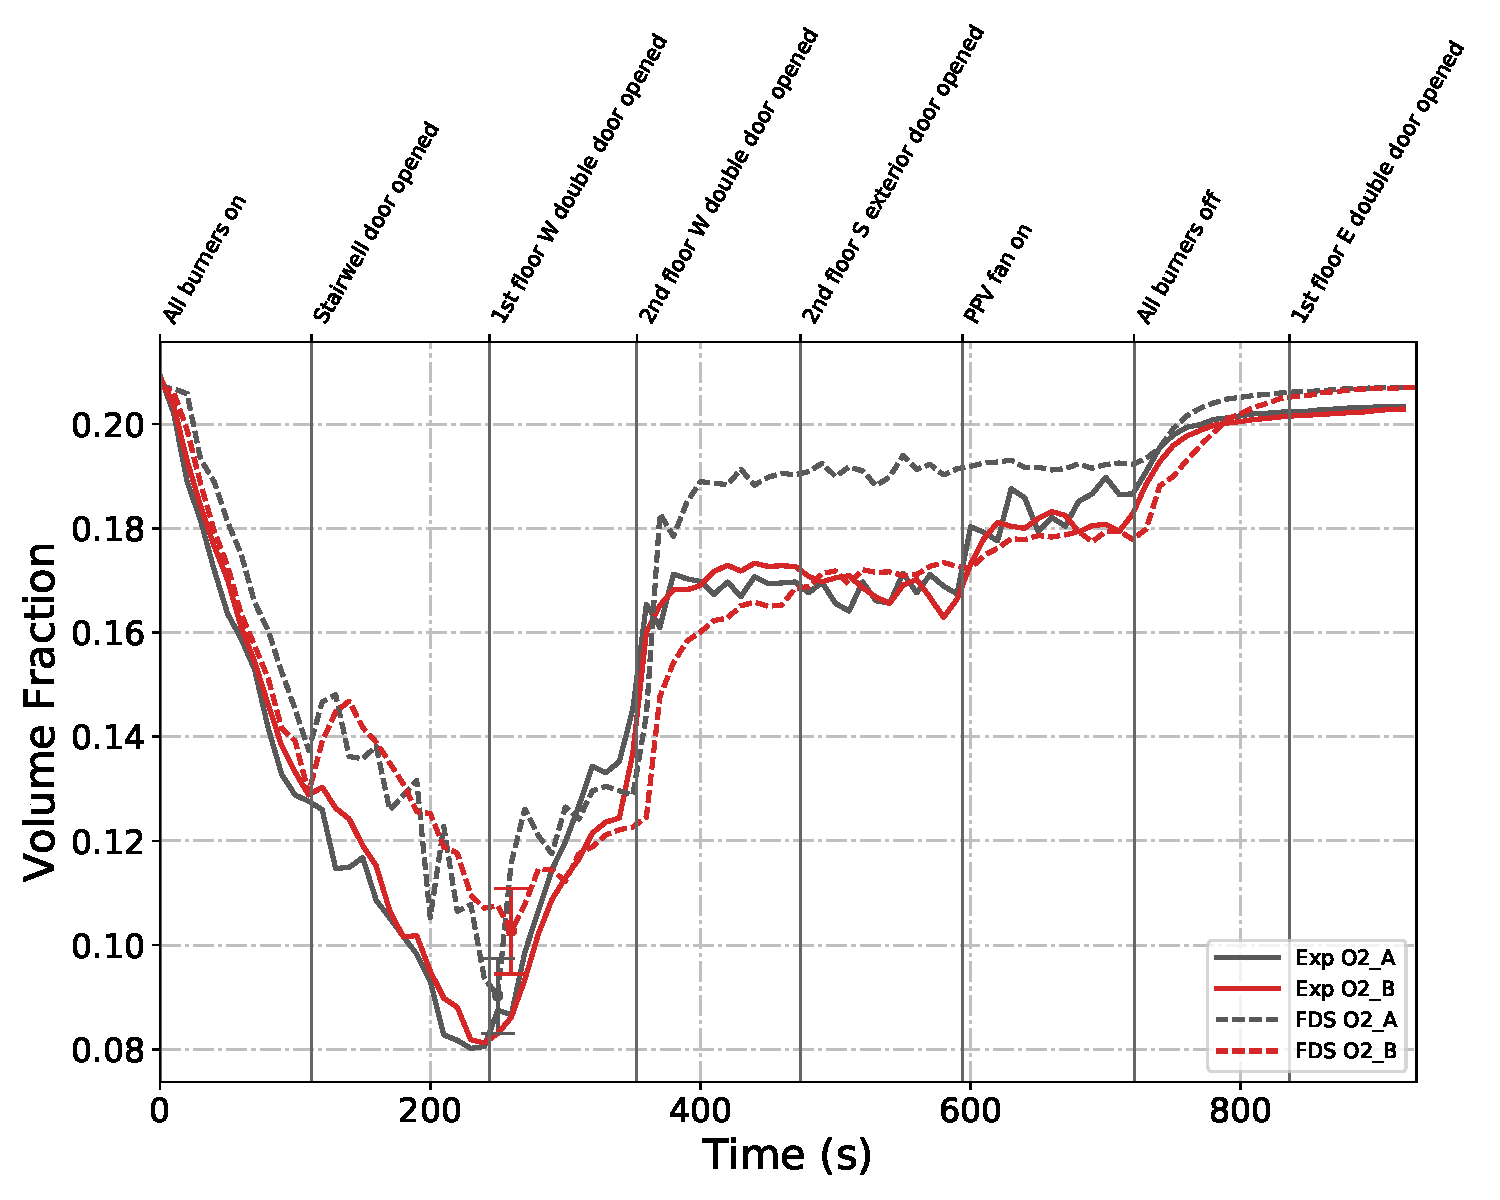
\includegraphics[width=\columnwidth]{../../Plots/Validation/Gas_Concentration/Test_25_O2}
	\caption[Plots of measured and predicted $O_2$ concentration during Test~25.]{Plots of measured and predicted $O_2$ concentration on the first floor (black plots) and second floor (red plots) of the West Structure during Test~25.}
	\label{fig:Test25_O2}
\end{figure}

\clearpage
\subsection*{\textit{CO$_2$ Concentration}}
\begin{figure}[!h]
	\centering
	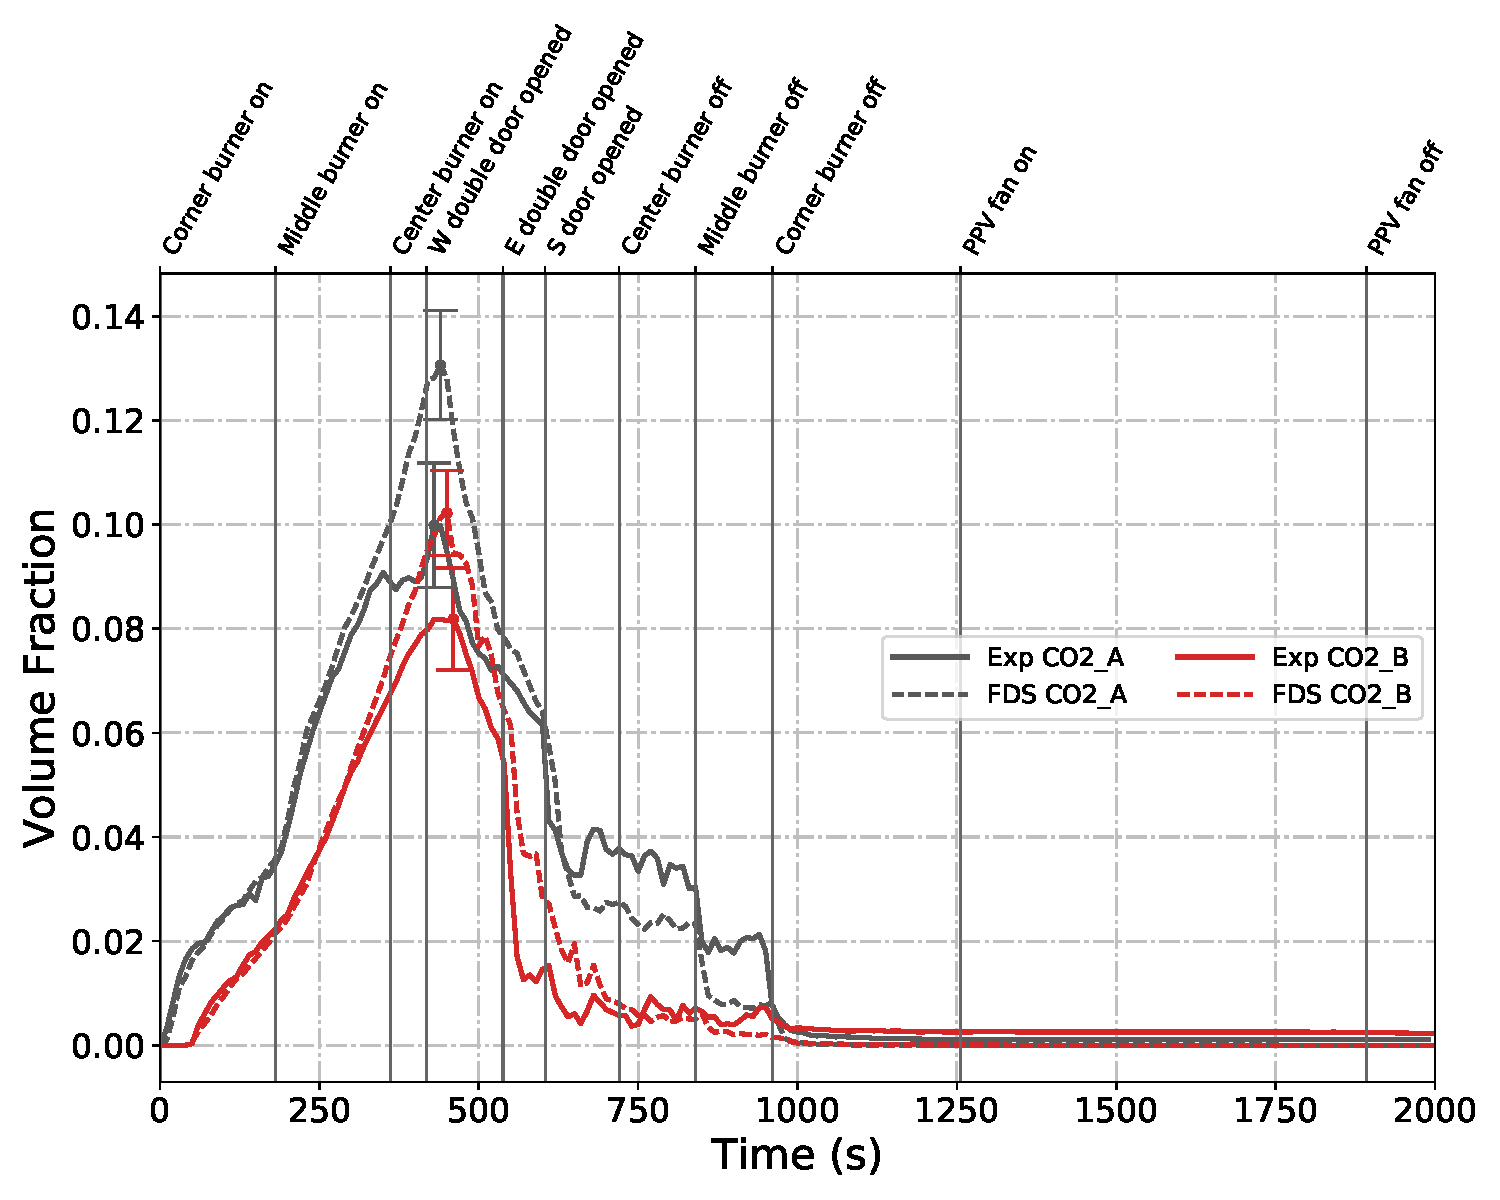
\includegraphics[width=\columnwidth]{../../Plots/Validation/Gas_Concentration/Test_2_CO2}
	\caption[Plots of measured and predicted $CO_2$ concentration during Test~2.]{Plots of measured and predicted $CO_2$ concentration in the fire room (black plots) and north room (red plots) of the East Structure during Test~2.}
	\label{fig:Test2_CO2}
\end{figure}

\begin{figure}[!h]
	\centering
	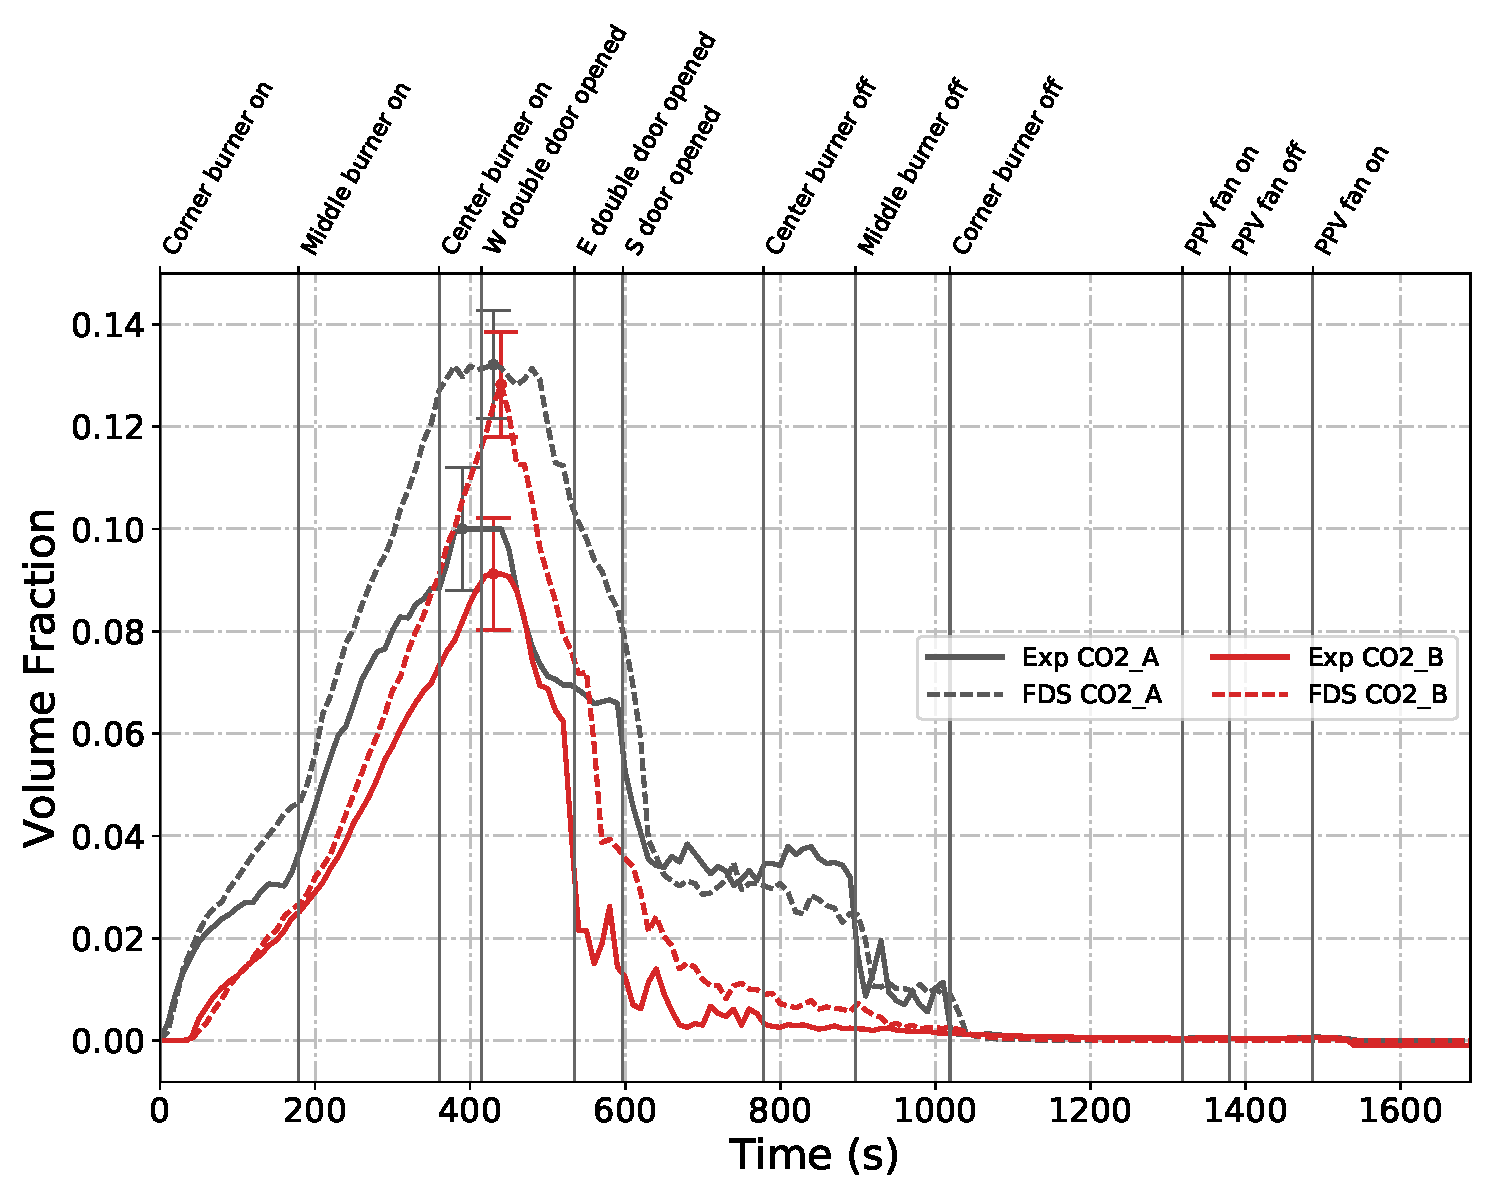
\includegraphics[width=\columnwidth]{../../Plots/Validation/Gas_Concentration/Test_4_CO2}
	\caption[Plots of measured and predicted $CO_2$ concentration during Test~4.]{Plots of measured and predicted $CO_2$ concentration in the fire room (black plots) and north room (red plots) of the East Structure during Test~4.}
	\label{fig:Test4_CO2}
\end{figure}

\begin{figure}[!h]
	\centering
	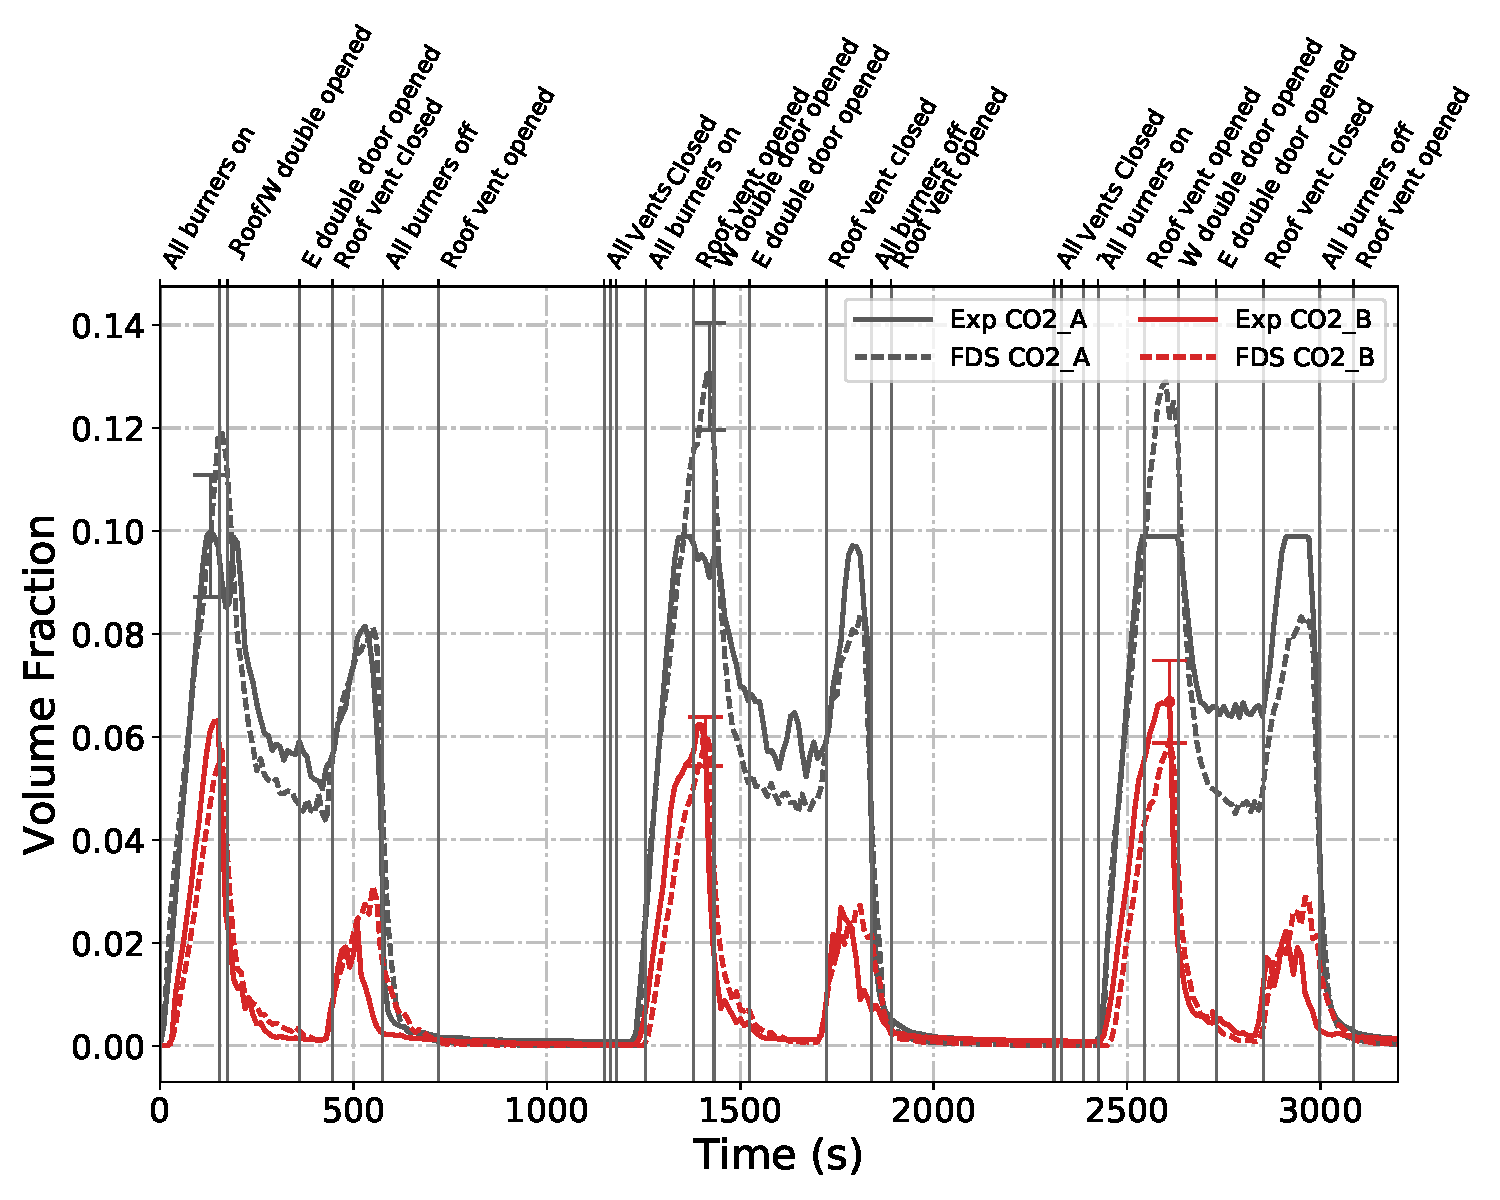
\includegraphics[width=\columnwidth]{../../Plots/Validation/Gas_Concentration/Test_5_CO2}
	\caption[Plots of measured and predicted $CO_2$ concentration during Test~5.]{Plots of measured and predicted $CO_2$ concentration in the fire room (black plots) and north room (red plots) of the East Structure during Test~5.}
	\label{fig:Test5_CO2}
\end{figure}

\begin{figure}[!h]
	\centering
	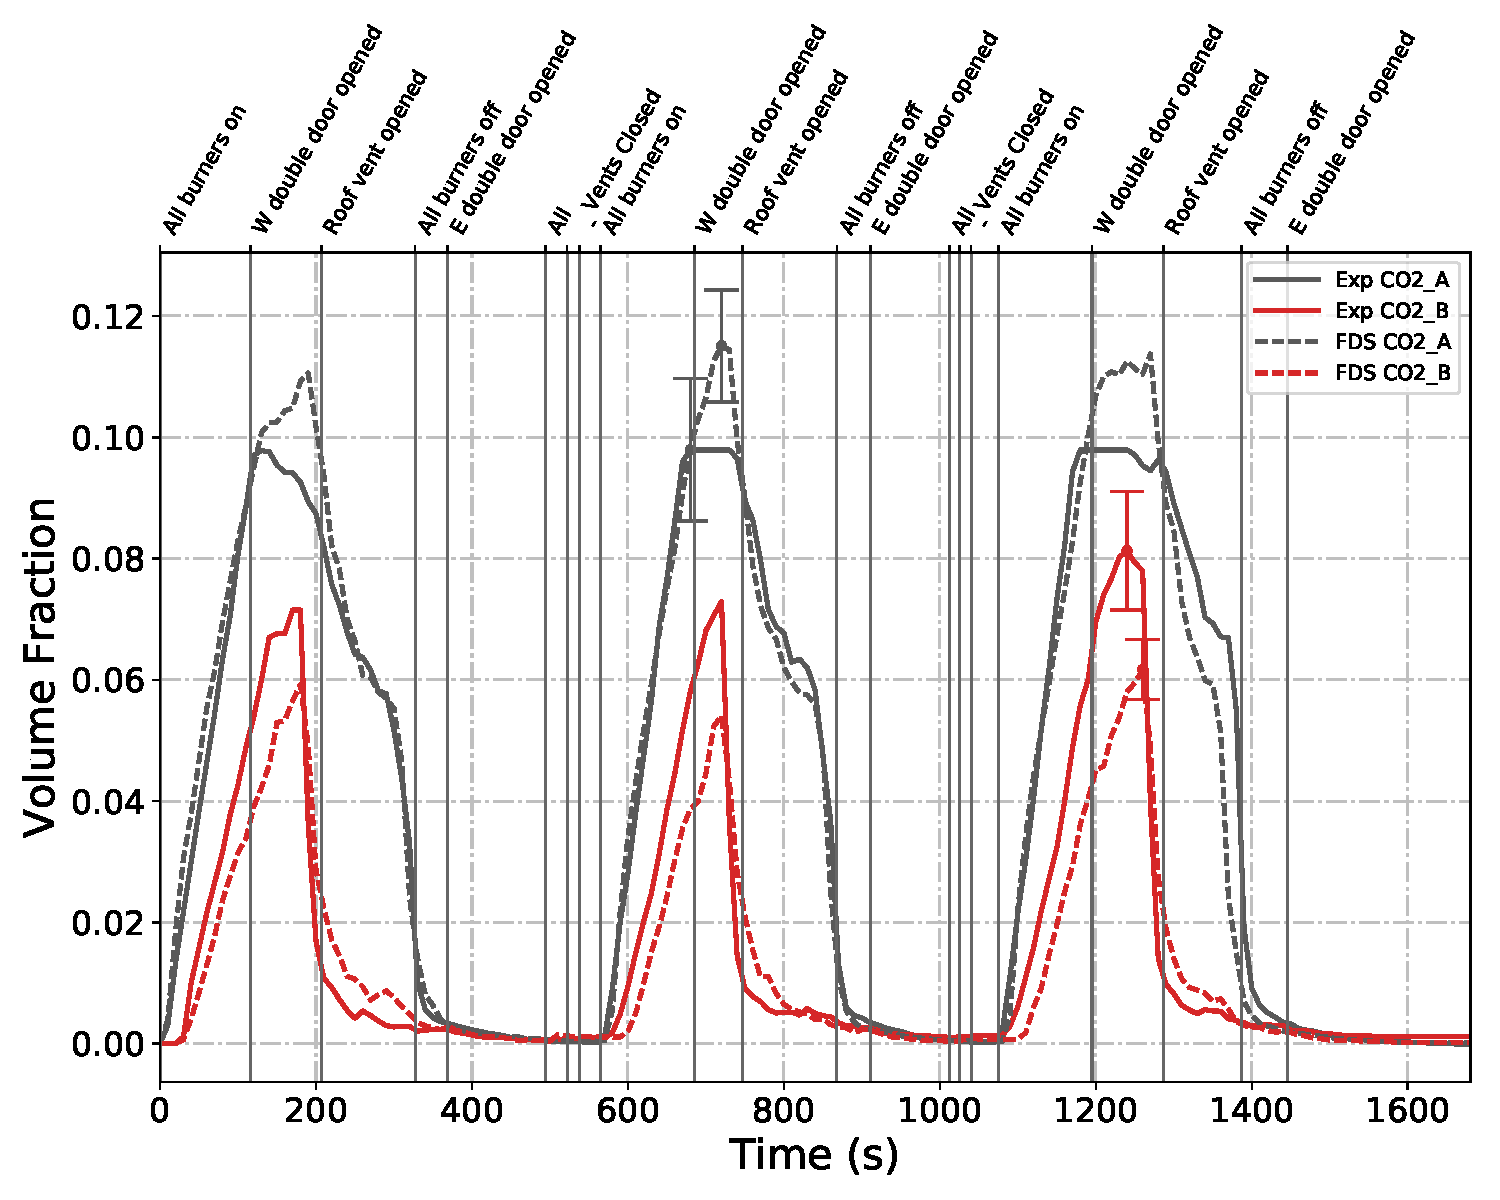
\includegraphics[width=\columnwidth]{../../Plots/Validation/Gas_Concentration/Test_6_CO2}
	\caption[Plots of measured and predicted $CO_2$ concentration during Test~6.]{Plots of measured and predicted $CO_2$ concentration in the fire room (black plots) and north room (red plots) of the East Structure during Test~6.}
	\label{fig:Test6_CO2}
\end{figure}

\begin{figure}[!h]
	\centering
	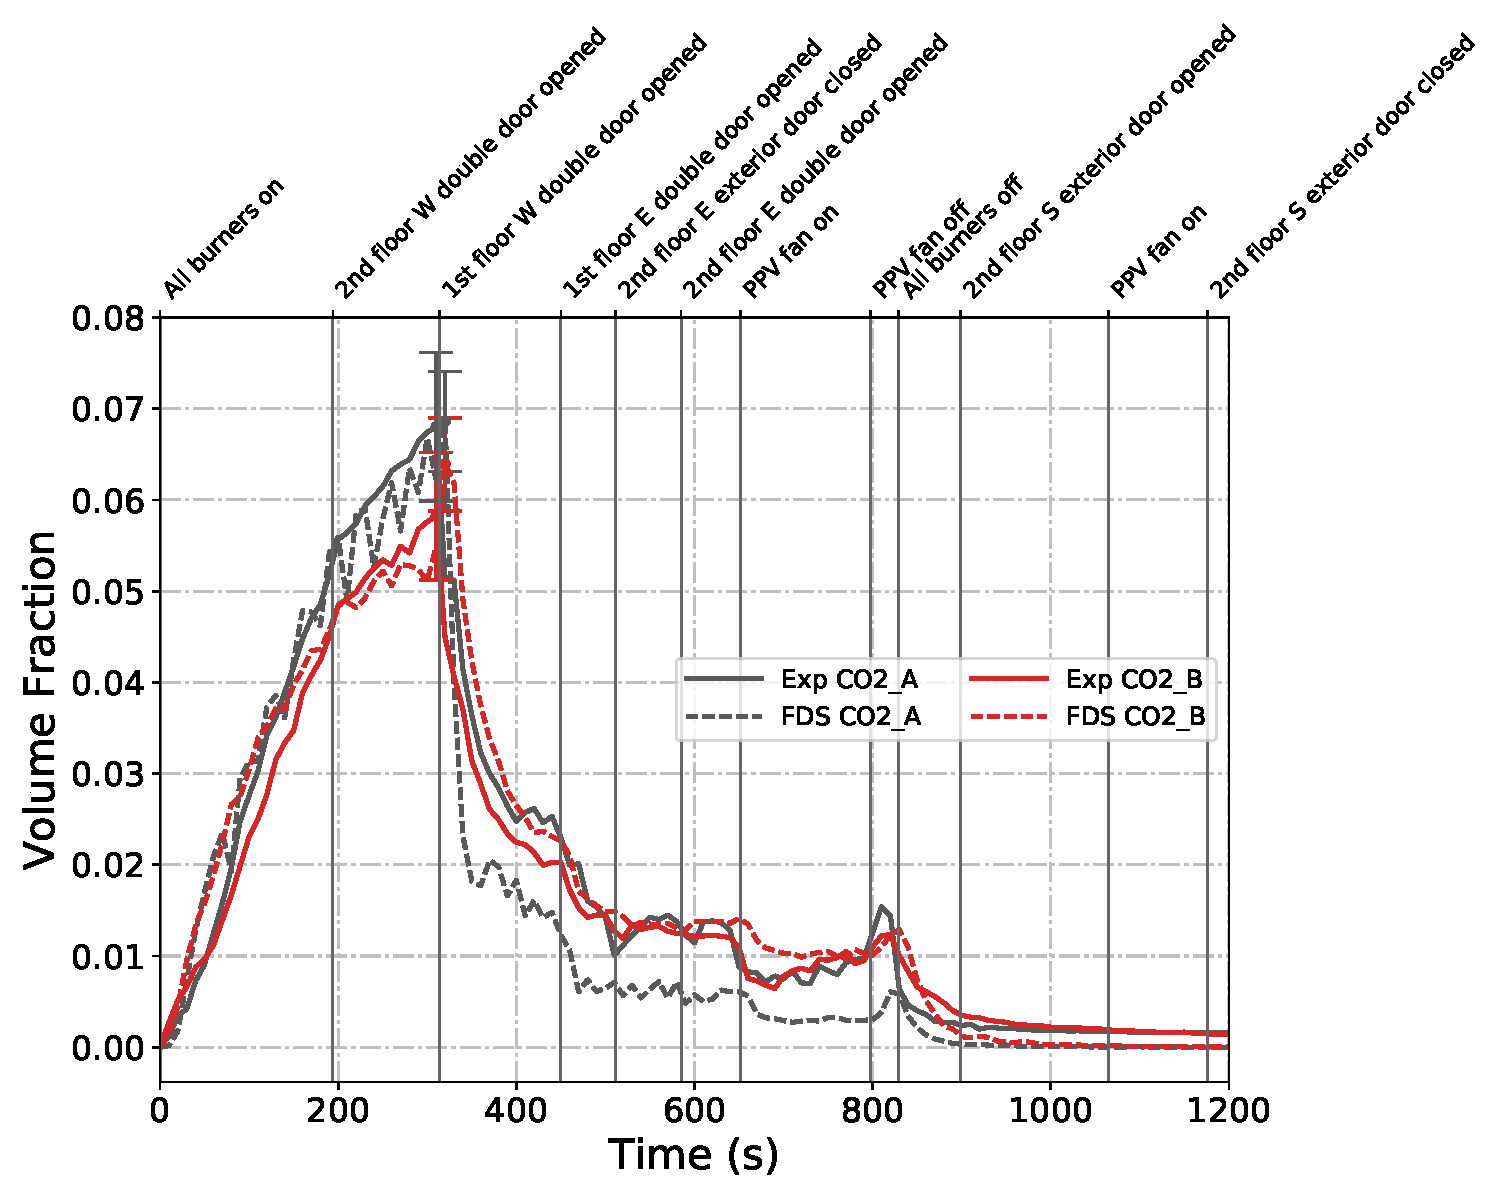
\includegraphics[width=\columnwidth]{../../Plots/Validation/Gas_Concentration/Test_22_CO2}
	\caption[Plots of measured and predicted $CO_2$ concentration during Test~22.]{Plots of measured and predicted $CO_2$ concentration on the first floor (black plots) and second floor (red plots) of the West Structure during Test~22.}
	\label{fig:Test22_CO2}
\end{figure}

\begin{figure}[!h]
	\centering
	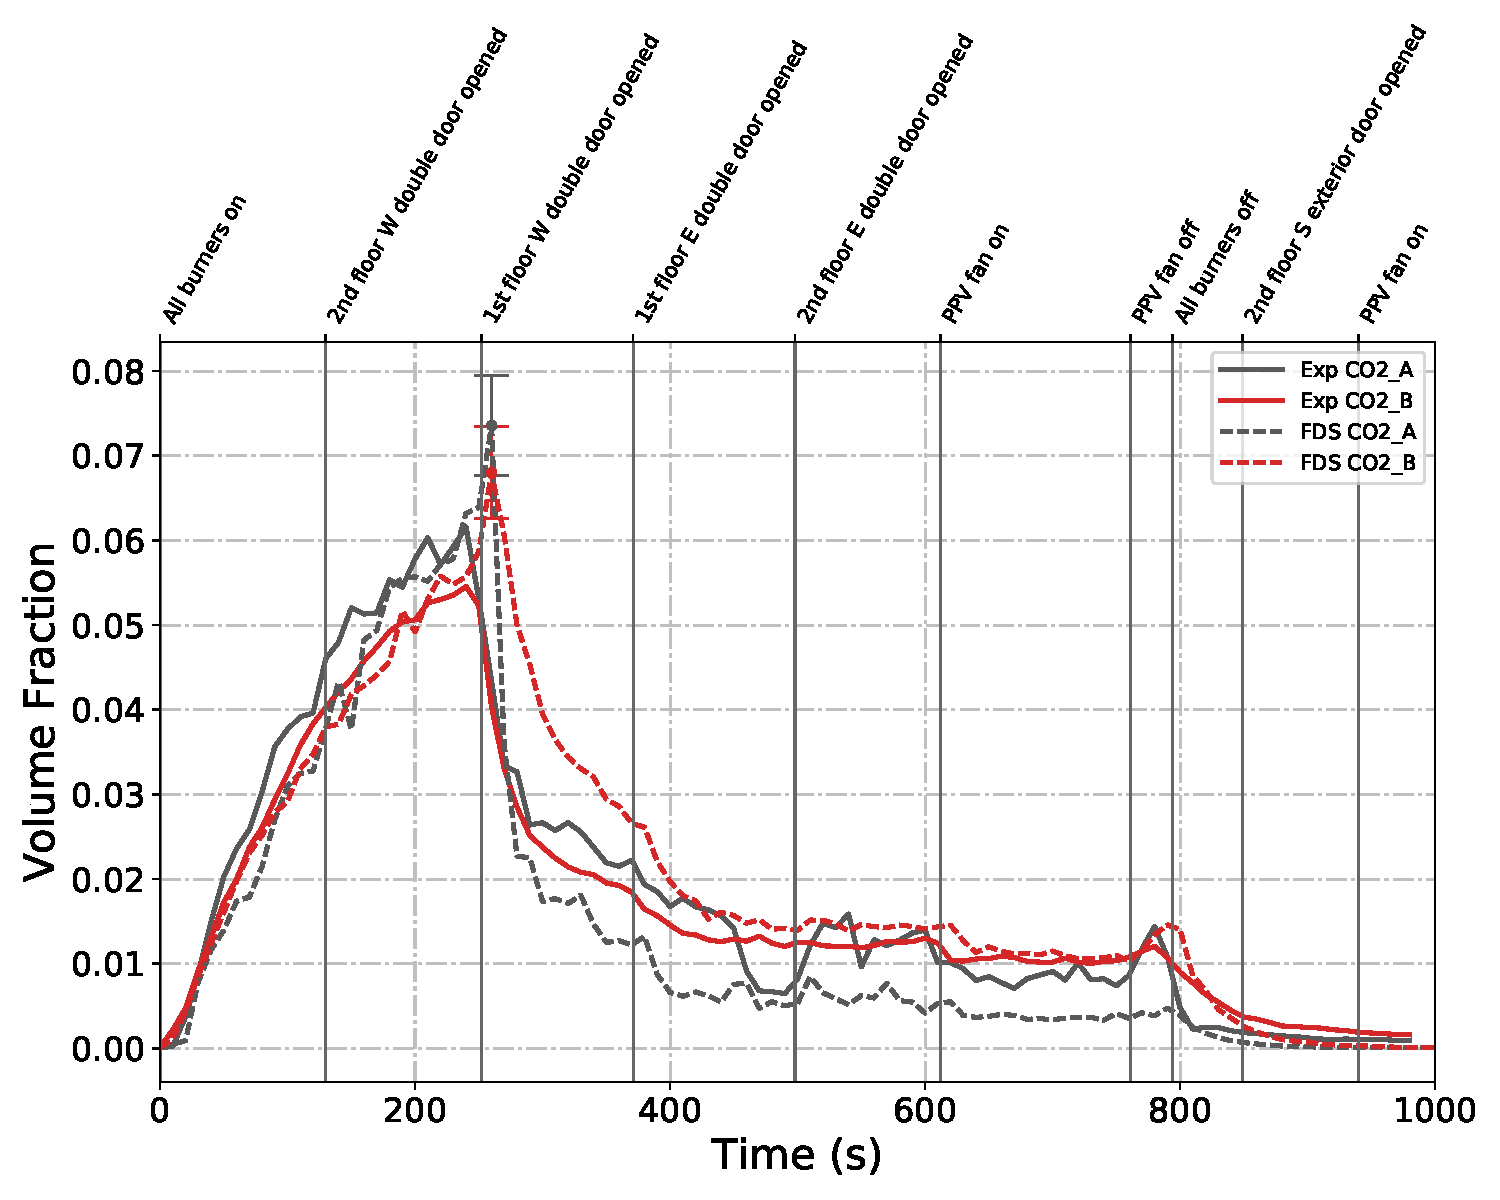
\includegraphics[width=\columnwidth]{../../Plots/Validation/Gas_Concentration/Test_23_CO2}
	\caption[Plots of measured and predicted $CO_2$ concentration during Test~23.]{Plots of measured and predicted $CO_2$ concentration on the first floor (black plots) and second floor (red plots) of the West Structure during Test~23.}
	\label{fig:Test23_CO2}
\end{figure}

\begin{figure}[!h]
	\centering
	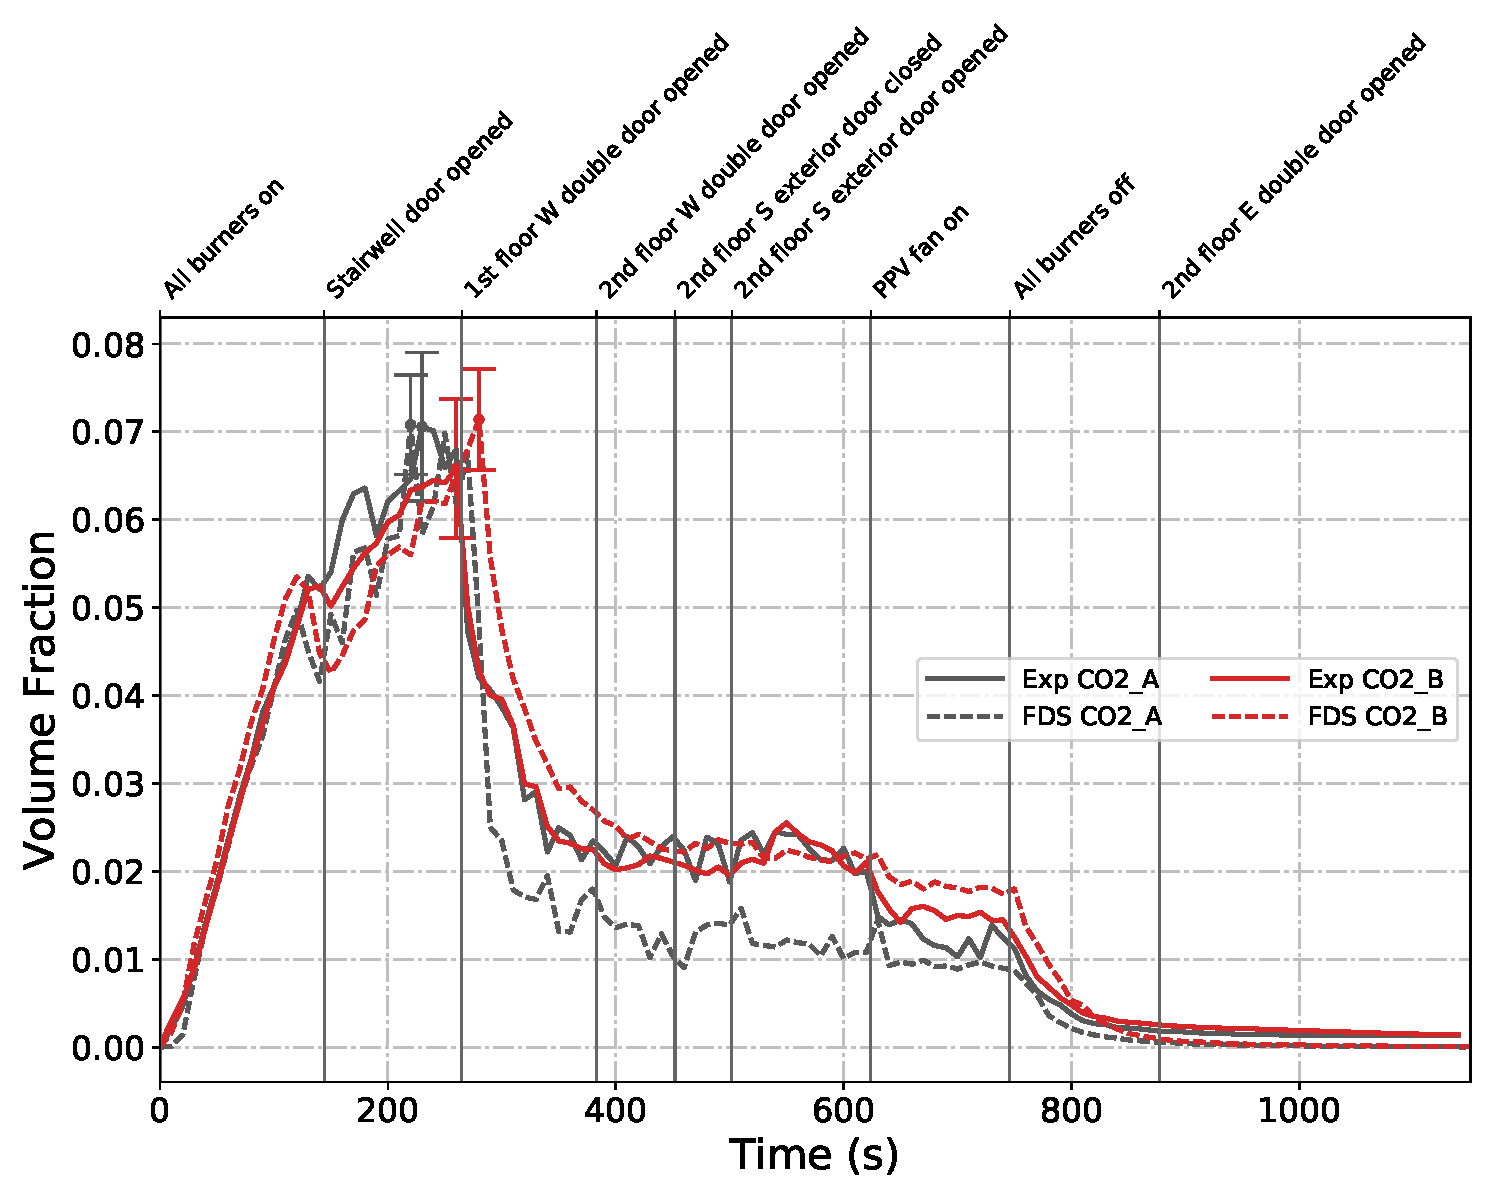
\includegraphics[width=\columnwidth]{../../Plots/Validation/Gas_Concentration/Test_24_CO2}
	\caption[Plots of measured and predicted $CO_2$ concentration during Test~24.]{Plots of measured and predicted $CO_2$ concentration on the first floor (black plots) and second floor (red plots) of the West Structure during Test~24.}
	\label{fig:Test24_CO2}
\end{figure}

\begin{figure}[!h]
	\centering
	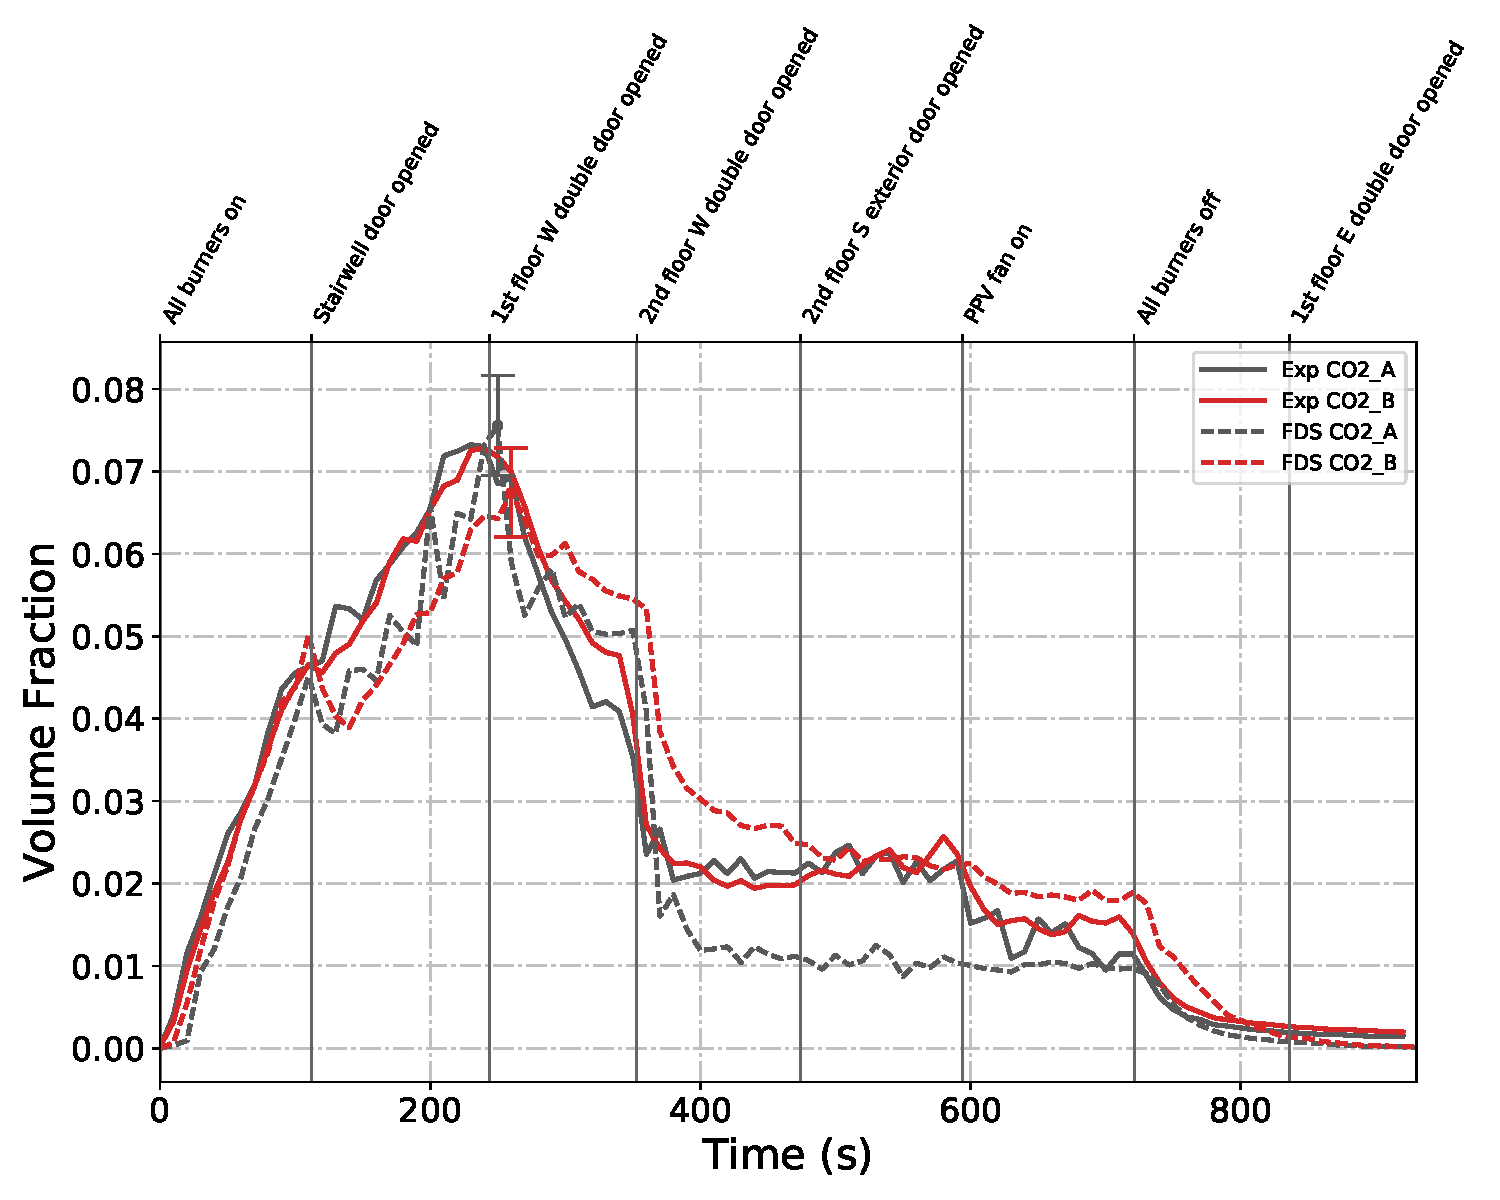
\includegraphics[width=\columnwidth]{../../Plots/Validation/Gas_Concentration/Test_25_CO2}
	\caption[Plots of measured and predicted $CO_2$ concentration during Test~25.]{Plots of measured and predicted $CO_2$ concentration on the first floor (black plots) and second floor (red plots) of the West Structure during Test~25.}
	\label{fig:Test25_CO2}
\end{figure}

\clearpage
\section{Gas Velocity}
\begin{figure}[!h]
	\centering
	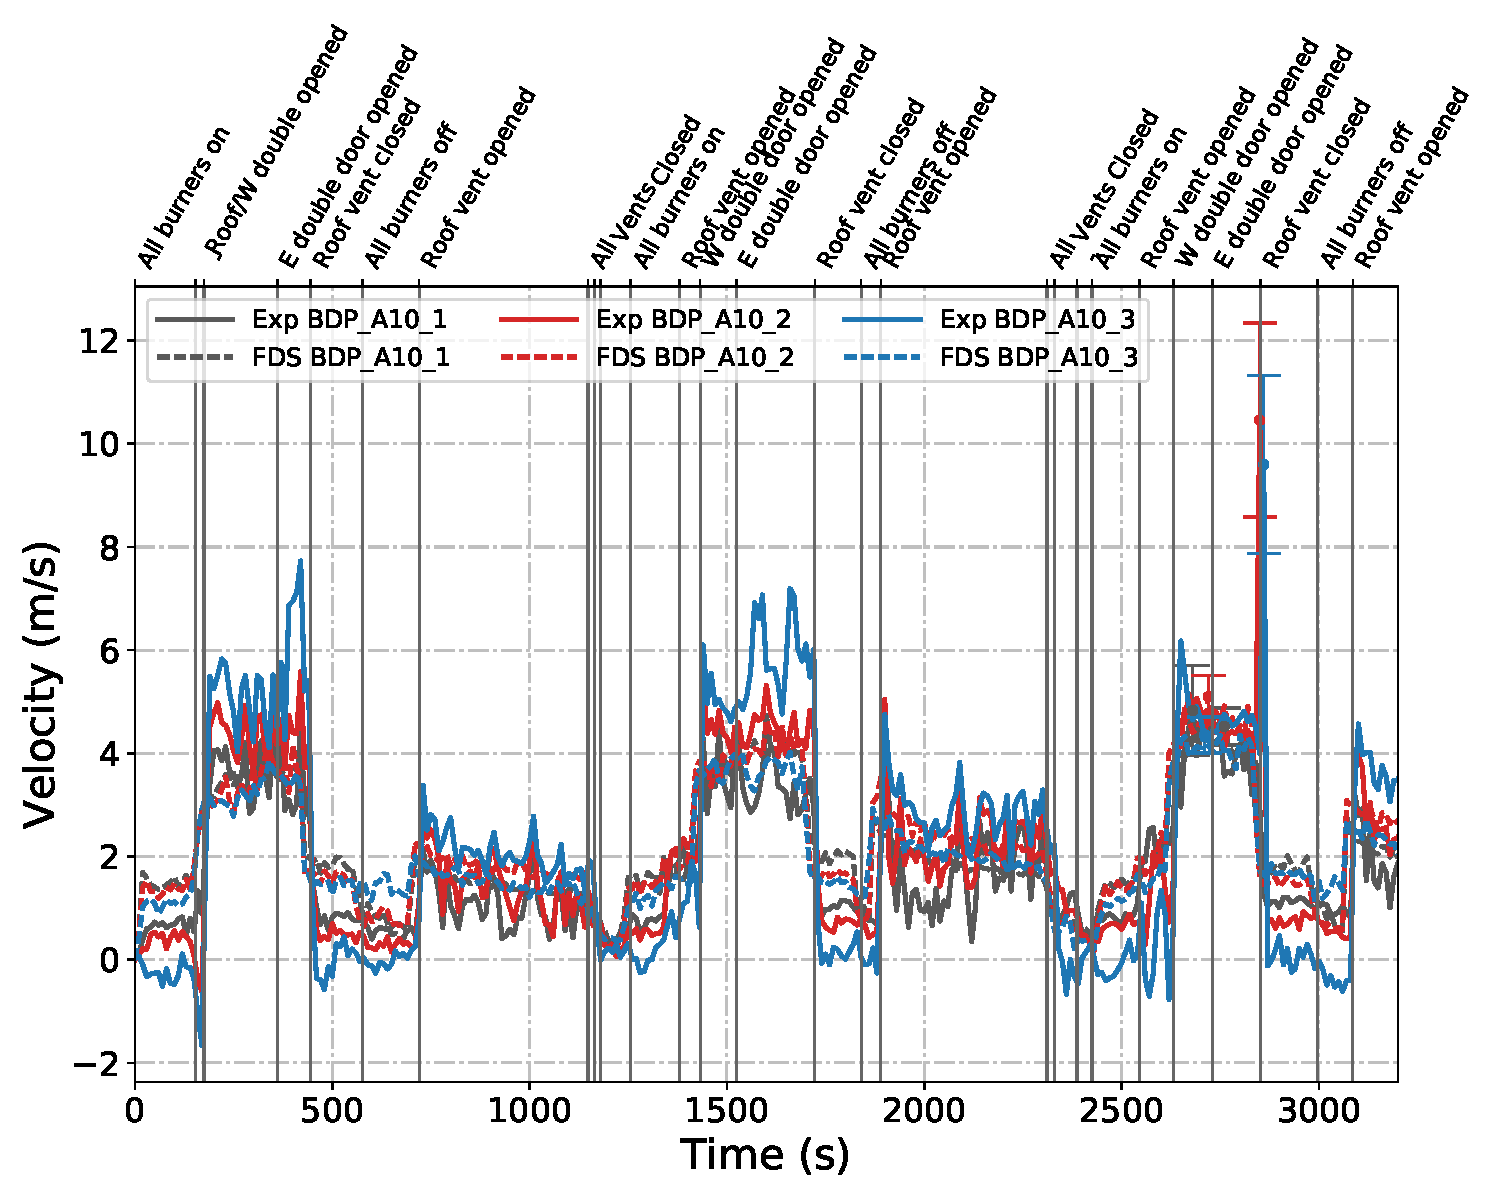
\includegraphics[width=\columnwidth]{../../Plots/Validation/Velocity/Test_5_BDP_A10}
	\caption[Plots of measured and predicted gas velocity through the roof vent during Test~5.]{Plots of measured and predicted gas velocity through the roof vent during Test~5.}
	\label{fig:Test5_BDPs}
\end{figure}

\clearpage
\section{Total Heat Flux}
\begin{figure}[!h]
	\centering
	\includegraphics[width=\columnwidth]{../../Plots/Validation/Heat_Flux/Test_23_HF_1}
	\caption[Plots of measured and predicted heat flux during Test~23.]{Plots of measured and predicted heat flux measured by total heat flux gauges at the top of the stairs facing the stair doorway (`H') and facing the ceiling (`V').}
	\label{fig:Test5_BDPs}
\end{figure}
